
% ----------------------------------------------------------------------
%                   LATEX TEMPLATE FOR PhD THESIS
% ----------------------------------------------------------------------

% based on Harish Bhanderi's PhD/MPhil template, then Uni Cambridge
% http://www-h.eng.cam.ac.uk/help/tpl/textprocessing/ThesisStyle/
% corrected and extended in 2007 by Jakob Suckale, then MPI-CBG PhD programme
% and made available through OpenWetWare.org - the free biology wiki


%: Style file for Latex
% Most style definitions are in the external file PhDthesisPSnPDF.
% In this template package, it can be found in ./Latex/Classes/
\documentclass[twoside,11pt]{Latex/Classes/PhDthesisPSnPDF}


% PREAMBLE
% Contains additional packages and setup commands.
% VU Page layout settings
\textwidth 15cm
\textheight 22cm
\parindent 10pt
\oddsidemargin 0.85cm
\evensidemargin 0.37cm

% VU overflow settings
% https://www.overleaf.com/learn/latex/%5Chbadness?
% https://www.overleaf.com/learn/latex/%5Chfuzz
\hbadness=10000
\hfuzz=50pt

% VU line spacing settings
% https://www.overleaf.com/learn/latex/Paragraph_formatting#Line_spacing
\renewcommand\baselinestretch{1.2}
\baselineskip=18pt plus1pt


% VU font encoding default
% https://www.overleaf.com/learn/latex/Font_typefaces
\usepackage[T1]{fontenc}

% UTF8 File Encoding
% https://www.overleaf.com/learn/how-to/What_file_encodings_and_line_endings_should_I_use%3F
\usepackage[utf8]{inputenc}

% Makes text pretty
\usepackage[
    activate={true,nocompatibility},
    final,
    tracking=false,
    kerning=true,
    spacing=false,
    factor=1100,
    stretch=10,
    shrink=10,
]{microtype}

% Defines acronyms used throughout the thesis
% See: glossaries.tex
\usepackage[abbreviations]{glossaries-extra}
\setabbreviationstyle[acronym]{long-short}

% GLOSSARY ENTRIES
% Defines acronyms and descriptions for frequently used
% terminology present in this thesis.
% http://tug.ctan.org/macros/latex/contrib/glossaries/glossariesbegin.pdf

% Define a term like this:
% \newglossaryentry{⟨label⟩}
% {
%     name={⟨name⟩},
%     description={⟨description⟩},
%     ⟨other options⟩
% }

% Acronym Example
% \newabbreviation{svm}{svm}{support vector machine}


% --------------------------------------------------------------------------

\makeglossaries


% --------------------------- ABBREVIATIONS --------------------------------

\newabbreviation{soa}{SOA}{Service Oriented Architecture}
\newabbreviation{iot}{IoT}{Internet of Things}
\newabbreviation{qos}{QoS}{Quality of Service}
\newabbreviation{kpi}{KPI}{Key Performance Indicator}
\newabbreviation{json}{JSON}{JavaScript Object Notation}
\newabbreviation{aip}{AIP}{Article Information Parser}
\newabbreviation{mcs}{MCS}{Massivizing Computer Systems}




%-------------------------- END ABBREVIATIONS ------------------------------




% ----------------------------- GLOSSARIES ---------------------------------

\newglossaryentry{sm}
{
    name={service mesh},
    plural={service meshes},
    description={A service mesh is a dedicated infrastructure layer that that abstracts the network layer between (micro)-services, to introduce distributed systems' best practices such as observability, traffic management, and security in a uniform way.}
}

\newglossaryentry{edge-computing}
{
    name={edge eomputing},
    description={A distributed computing paradigm that brings computation and data storage closer to the sources of data.}
}

\newglossaryentry{smi}
{
    name={Service Mesh Interface},
    description={A standard interface for service meshes on Kubernetes, which covers the most common service mesh capabilities such as traffic policies, traffic telemetry and traffic management.}
}

\newglossaryentry{smp}
{
    name={Service Mesh Performance},
    description={A common format to capture and describe configurations and results of service mesh performance experiments.}
}

\newglossaryentry{fr}
{
    name={Functional Requirement},
    description={A a requirement that specifies criteria that can be used to judge the operation of a system, rather than specific behaviors.}
}


\newglossaryentry{nfr}
{
    name={Non-Functional Requirement},
    description={A a requirement that specifies criteria that can be used to judge the operation of a system, rather than specific behaviors.}
}

\newglossaryentry{cncf}
{
    name={Cloud Native Computing Foundation},
    description={A Linux Foundation project that was founded in 2015 to help advance container technology and align the tech industry around its evolution in a vendor neutral fashion.}
}

\newglossaryentry{pl}
{
    name={Primary Literature},
    description={The immediate results of research activities by scientists.}
}

\newglossaryentry{gl}
{
    name={Grey Literature},
    description={The materials and research produced by organizations outside of the traditional commercial or academic publishing.}
}

\newglossaryentry{slr}
{
    name={Systematic Literature Review},
    description={A type of literature review that uses repeatable analytical methods to collect and analyze data.}
}

\newglossaryentry{mlr}
{
    name={Multivocal Literature Review},
    description={A form of systematic literature reviews that includes \gls{gl} in addition to the formal \gls{pl}.}
}

\newglossaryentry{backward-snowballing}
{
    name={Backward Snowballing},
    description={A form of systematic literature reviews that includes \gls{gl} in addition to the formal \gls{pl}.}
}

\newglossaryentry{devops}
{
    name={DevOps},
    description={A set of software development (dev) and it operations (ops) practices which aim to shorten the systems development life cycle and provide continuous delivery with high software quality.}
}

\newglossaryentry{container}
{
    name={container},
    description={A unit of software packaging that combines the software and all of its dependencies in a standard format.}
}

\newglossaryentry{docker}
{
    name={Docker},
    description={A software platform used to create, run and manage software applications packaged in \glspl{container}.}
}

\newglossaryentry{vm}
{
    name={virtual machine},
    description={A software based, virtualization of a computer system.}
}

\newglossaryentry{micro-service}
{
    name={micro-service},
    description={A variant of the \gls{soa} architectural style with fine-grained services and ligthweight protocols.}
}

\newglossaryentry{k8s}
{
    name={Kubernetes},
    description={An open-source \gls{container} orchestration system for automating software deployment, scaling, and management.}
}

\newglossaryentry{monolith}
{
    name={monolith},
    description={A software architecture that is self-contained and where the user interface and data access paterns are combined into a single program.}
}

\newglossaryentry{esb}
{
    name={Enterprise Service Bus},
    description={An Enterprise Service Bus is an open standards, message-based, distributed integration infrastructure that provides routing, invocation and mediation services to facilitate the interactions of disparate distributed applications and services in a secure and reliable manner \cite{menge2007enterprise}.}
}

\newglossaryentry{ebpf}
{
    name={eBPF},
    description={eBPF (extended Berkeley Packet Filter), is a technology which allows to run sandboxed programs in the Linux Kernel. It can do so without changing the kernel source code or loading kernel modules.}
}

\newglossaryentry{linkerd}
{
    name={Linkerd},
    description={A service mesh implementation by Buoyant.}
}

\newglossaryentry{grpc}
{
    name={gRPC},
    description={A a modern open source high performance Remote Procedure Call (RPC) framework.}
}

\newglossaryentry{pod}
{
    name={Pod},
    description={The smallest deployable units of computing that you can create and manage in Kubernetes, consists of one or more application containers.}
}

\newglossaryentry{sut}
{
    name={System Under Test},
    description={A system that is being tested for correct operation}
}

\newglossaryentry{gcp}
{
    name={Google Cloud Platform},
    description={Google's offering for various cloud compute services}
}

\newglossaryentry{gke}
{
    name={Google Kubernetes Engine},
    description={A managed kubernetes service offered by Google on their Google Cloud Platform service.}
}

\newglossaryentry{aws}
{
    name={Amazon Web Services},
    description={Amazon's offering for various cloud compute services}
}




% \newglossaryentry{soa}
% {
%     name={Service Oriented Architecture},
%     description={A software development approach that takes advantages of decoupling software components into independent and reusable services.}
% }

\newglossaryentry{sla}
{
    name={Service-Level Agreement},
    plural={Service-Level Agreements},
    description={A commitment between a service provider and a client.}
}

\newglossaryentry{turnip}
{
    name={turnip},
    description={round pale root vegetable}
}

\newglossaryentry{carrot}
{
    name={carrot},
    description={orange root}
}

% --------------------------- END GLOSSARIES -------------------------------


\usepackage{amsmath, amsthm, amssymb} % American Math Society packages
\usepackage{pifont} % Symbols etc.
\usepackage{pdfpages} % Insert PDF pages into latex documents
\usepackage{tikz} % Package for creating graphics
\usepackage{booktabs} % Nicer tables
\usepackage{xcolor} % Enables coloured text
\usepackage{minted} % Code listings
\usepackage[noabbrev, capitalise]{cleveref} % Uniform (smart) references
\usepackage{todonotes} % Enables visual todonotes
\usepackage{enumitem} % Spacing in enumerations
\usepackage{url} % Clickable and formatted urls
\usepackage{listings} % Source code printer

% Checkmark and X
\newcommand{\cmark}{\ding{51}}%
\newcommand{\xmark}{\ding{55}}%


\setuptodonotes{
    inline,
    color=red!40,
}







  

\begin{document}

% ----------------------------------------------------------------------



%: ----------------------------------------------------------------------
%:                  TITLE PAGE: name, degree,..
% ----------------------------------------------------------------------
%: ----------------------------------------------------------------------
%:                  TITLE PAGE: name, degree,..
% ----------------------------------------------------------------------
\thispagestyle{empty}

\begin{center}
Vrije Universiteit Amsterdam \hspace*{2cm} Universiteit van Amsterdam

\vspace{1mm}

\hspace*{-7.5cm}
\includegraphics[height=25mm]{vu-griffioen}

\vspace*{-2cm}\hspace*{7.5cm}
\includegraphics[height=15mm]{uva_logo}

\vspace{2cm}

{\Large Master Thesis}

\vspace*{1.5cm}

\rule{.9\linewidth}{.6pt}\\[0.4cm]
{\huge \bfseries 
    Experimental Performance Analysis of Service Mesh Systems
\par}\vspace{0.4cm}
\rule{.9\linewidth}{.6pt}\\[1.5cm]

\vspace*{2mm}

{\Large
\begin{tabular}{l}
{\bf Author:} ~~Richard Bieringa~~~~ (2544975)
\end{tabular}
}

\vspace*{1cm}

\begin{tabular}{ll}
{\it 1st supervisor:}   & ~~Prof. dr. ir. Alexandru Iosup \\
{\it daily supervisor:} & ~~ir. Erwin van Eyk \\
{\it 2nd reader:}       & ~~dr. ir. Animesh Trivedi
\end{tabular}

\vspace*{1cm}

\textit{A thesis submitted in fulfillment of the requirements for\\ the joint UvA-VU Master of Science degree in Computer Science}

\vspace*{1.8cm}

\today\\[4cm] % Date

\end{center}


%: --------------------------------------------------------------
%:                  FRONT MATTER: dedications, abstract,..
% --------------------------------------------------------------


%\language{english}




%: ----------------------- generate cover page ------------------------

\begin{center}
\textit{``I've always believed that you should never ever give up and you should always keep fighting even when there's only a slightest chance.'' \\ by Michael Schumacher}
\end{center}

%: ----------------------- cover page back side ------------------------
% Your research institution may require reviewer names, etc.
% This cover back side is required by Dresden Med Fac; uncomment if needed.


%: ----------------------- TODO notes ------------------------

% This is page to keep track of all the todo notes in the document.
% Should be removed/commented before finalizing the document.



%: ----------------------- abstract ------------------------

% Your institution may have specific regulations if you need an abstract and where it is to be placed in the document. The default here is just after title.


% Thesis Abstract -----------------------------------------------------


%\begin{abstractslong}    %uncommenting this line, gives a different abstract heading
\begin{abstracts}        %this creates the heading for the abstract page
Service-oriented computing, an architectural approach of decomposing software into logical services, has seen an increase in popularity over the past decades. Later forms, such as the widely popular microservices-based architecture is an evolution of service-oriented computing made possible by the reductions in deployment costs and resource overhead. These architectures offer advantageous characteristics, such as an increase in flexibility and scalability. However, due to its design, it also introduces an additional layer of complexity due to the overhead in communication and the inherent reliability issues from networks. The service mesh architecture tries aims to solve these issues whilst providing a uniform way of handling security, observability, and reliability concerns without modifying application code. In this thesis, we dissect the state-of-the service mesh systems and identify three different service mesh architectures. Furthermore, we design \textit{Mesh Bench} a benchmark used to evaluate the performance characteristics of service mesh systems. We implement a prototype of the benchmark and take an experimental approach to evaluating the most popular service mesh implementations in the form of \textit{Istio} and \textit{Linkerd}, and implementations using vastly different architectures in the form of \textit{Cilium} and \textit{Traefik mesh}. Based on the results of the performance experiments we uncover the performance overheads of service mesh systems and identify promising, future directions and evolutions of the techonology.

\end{abstracts}
%\end{abstractlongs}


% ---------------------------------------------------------------------- 


% The original template provides and abstractseparate environment, if your institution requires them to be separate. I think it's easier to print the abstract from the complete thesis by restricting printing to the relevant page.
% \begin{abstractseparate}
%   
% Thesis Abstract -----------------------------------------------------


%\begin{abstractslong}    %uncommenting this line, gives a different abstract heading
\begin{abstracts}        %this creates the heading for the abstract page
Service-oriented computing, an architectural approach of decomposing software into logical services, has seen an increase in popularity over the past decades. Later forms, such as the widely popular microservices-based architecture is an evolution of service-oriented computing made possible by the reductions in deployment costs and resource overhead. These architectures offer advantageous characteristics, such as an increase in flexibility and scalability. However, due to its design, it also introduces an additional layer of complexity due to the overhead in communication and the inherent reliability issues from networks. The service mesh architecture tries aims to solve these issues whilst providing a uniform way of handling security, observability, and reliability concerns without modifying application code. In this thesis, we dissect the state-of-the service mesh systems and identify three different service mesh architectures. Furthermore, we design \textit{Mesh Bench} a benchmark used to evaluate the performance characteristics of service mesh systems. We implement a prototype of the benchmark and take an experimental approach to evaluating the most popular service mesh implementations in the form of \textit{Istio} and \textit{Linkerd}, and implementations using vastly different architectures in the form of \textit{Cilium} and \textit{Traefik mesh}. Based on the results of the performance experiments we uncover the performance overheads of service mesh systems and identify promising, future directions and evolutions of the techonology.

\end{abstracts}
%\end{abstractlongs}


% ---------------------------------------------------------------------- 

% \end{abstractseparate}


%: ----------------------- tie in front matter ------------------------

\frontmatter
% Thesis Dedication ---------------------------------------------------

%\begin{dedication} %this creates the heading for the dedication page

%To ...

%\end{dedication}

% ----------------------------------------------------------------------
% Thesis Acknowledgements ------------------------------------------------


%\begin{acknowledgementslong} %uncommenting this line, gives a different acknowledgements heading
%\begin{acknowledgements}      %this creates the heading for the acknowlegments


%\end{acknowledgements}
%\end{acknowledgmentslong}

% ------------------------------------------------------------------------





%: ----------------------- contents ------------------------

\setcounter{secnumdepth}{3} % organisational level that receives a numbers
\setcounter{tocdepth}{1}    % print table of contents for level 3
\tableofcontents            % print the table of contents
% levels are: 0 - chapter, 1 - section, 2 - subsection, 3 - subsection


%: ----------------------- list of figures/tables ------------------------

\listoffigures	% print list of figures

\listoftables  % print list of tables




%: ----------------------- glossary ------------------------

% Tie in external source file for definitions: /0_frontmatter/glossary.tex
% Glossary entries can also be defined in the main text. See glossary.tex
% 
%\include{0_frontmatter/glossary} 

%\begin{multicols}{2} % \begin{multicols}{#columns}[header text][space]
%\begin{footnotesize} % scriptsize(7) < footnotesize(8) < small (9) < normal (10)

%\printnomenclature[1.5cm] % [] = distance between entry and description
%\label{nom} % target name for links to glossary

%\end{footnotesize}
%\end{multicols}



%: --------------------------------------------------------------
%:                  MAIN DOCUMENT SECTION
% --------------------------------------------------------------

% the main text starts here with the introduction, 1st chapter,...
\mainmatter

\renewcommand{\chaptername}{} % uncomment to print only "1" not "Chapter 1"


%: ----------------------- subdocuments ------------------------

% Parts of the thesis are included below. Rename the files as required.
% But take care that the paths match. You can also change the order of appearance by moving the include commands.

% Setup
\graphicspath{./figures}

\chapter{Introduction}
\label{chap:introduction}

% Introduction

A \gls{sm} is a dedicated layer of infrastructure that sits between services and aims to provide several distributed systems best practices in a uniform manner. The terminology was introduced in the last decade, and several implementations have seen the light of day since. The premise of introducing additional observability in the system, increasing the reliability of it while also adding security best practices to little or no additional lines of application code made this technology a hot topic in the field. However, this technology does not come in the form of a zero cost offering. Most of the service mesh designs work by introducing additional network proxies and an additional control plane. By introducing these components into the system, an increase in system resources is to be expected. More importantly, the introduction of a proxy between each service leads to additional latencies in every service-to-service communication. 

The introduction of additional latencies in service-to-service communications or the increase in system resources can be a make or break scenario in many aspects. Companies and organizations for example can have \gls{kpi} based on the end-to-end response times of the services they provide. These \gls{qos} based metrics are important and drive their business decisions. Can the introduction of the benefits provided by a \gls{sm} outweigh the additional latency introduced, or more importantly, how much latency will be introduced at all? Another scenario that comes to mind comes in the form of resource constrained environments, which can often occur in \gls{iot} or \gls{edge-computing} topologies. 

Although the technology has been in the spotlight in the last decade and the technology has seen a steady increase in adoption \cite{cncf-survey-2020, rh-survey} and implementations have seen to matured, there has been a lack of performance studies that evaluate these systems in depth. Previous works have established the groundwork by introducing simple benchmarking instruments \cite{kinvolk-bench} and their preliminary results \cite{bench-istio-linkerd-2019, bench-istio-linkerd-2021}. These benchmarks and instruments, however, do not capture the unique characteristics of a \gls{sm} well enough.

\todo{Fix intro last p (END)}
In this thesis, we present x, an automated service mesh evaluation benchmark that makes it easy to conduct reproducible real world experiments on different \gls{sm} implementations. With this instrument, we conduct experiments on existing \gls{sm} implementation to compare them on key performance characteristics.

% Sections 
\section{Context}
\label{sec:introduction:context}
% Societal impact
% Economic -> Impact for companies (e2e latencies)
% Society at large -> We rely on infra (shift in responsibilies)
% Companies involved



% Field imapct (Intellectual Argument)
% Industry -> Considerable resouces / Relatively little scientific output
% Shift from libary approach -> service meshes
% Emerging field, new tech (ebpf)
% Lots of new systems (OSM, Cilium)


% Why should people care about the  work
We live in the \textit{Age of Computer Ecosystems} \cite{Iosup2018}, where our society as a whole relies on the modern IT infrastructure. From governments to schools and businesses, many use the internet as a gateway to their services and offerings. The design of modern IT systems and infrastructure therefore has a large societal impact, for both the end user, the providing entities, and the every increasing number of engineers \cite{it-employment-worldwide} that are required to develop and manage it.

Businesses that rely on IT infrastructure, can face major economic impact through slight design alterations. Amazon, for example, found that for every 100ms of additional end-to-end latency, it would lose out on roughly 1\% of total sales revenue \cite{amazon-latency-conversion-drop}. And Google, indicated back in 2009 \cite{google-latency-bounce-rate} that latency has a direct relation with service usage and has been actively prioritizing performance of services ever since

In this thesis, we evaluate the \gls{sm} architecture and systems that implement this. These systems introduce an additional layer of machinery that naturally causes a performance overhead. Even though, the performance complications can have major impact, the systems in question have received lots of attention from the industry and increasing number of companies are evaluating and using such solutions in their IT infrastructure \cite{cncf-survey-2021}.  With large corporations, such as Google and Microsoft backing the development of \gls{sm} systems it is clear that this technology has lots of potential. 

The \gls{sm} landscape is a rapidly evolving field, that is in its relative infancy.  There have been numerous new systems that have emerged in the last couple of years and there have been many technological advancements that pave the way for alternative approaches to the problem. It comprises a landscape where most of the systems are in active development and see frequent improvements and architectural changes \cite{istio-merbridge, cilium-mesh}. This grants us the opportunity to evaluate the different approaches these systems take, as they evolve and explore an exciting field of bleeding-edge technologies.

Although \gls{sm} systems have gained a lot of attention and hype from within the industry. It has received relatively little to no attention from academia as observed by our previous works in which we have conducted a topical survey of the field. In this thesis, we aim to close that gap by performing an extensive study on \gls{sm} systems, with a focus on their performance characteristics.

% MCS relation
Throughout this thesis, we align ourselves with the goals and visions expressed in \gls{mcs} \cite{Iosup2018}. The work as presented in this thesis aims to uncover the intricacies of the computer ecosystems discussed, helping to understand them and guide future system designs. \gls{mcs} envisions a domain where everything developed is tested and benchmarked in a reproducible manner. This ideology is exemplified by the experimental approach used  throughout this thesis.2





\section{Problem Statement}
\label{sec:introduction:problem-statement}

% Intro problem 
% - Fast growing, but immature
% - Operational & performance challenges
% - - SMI / SMP
% - Non Functional Requirements
% - How to compare systems
% - Balance between performance/reliability


\Gls{sm} systems form a relatively new and exciting field, that is rapidly evolving. However, it is also a field where there is very limited output from the academic world. Specifically, there is very little known about the performance implications of these systems. The goal of this thesis is to answer this unsolved challenge, and perform an extensive study into performance implications of \gls{sm} systems. 

Although there has not been much attention from academia, prior efforts originating from the industry have resulted in a tool \cite{kinvolk-bench} that can capture performance overheads in \gls{sm} systems. This tool lacks in depth and scope, but has laid some groundwork by producing early performance results \cite{bench-istio-linkerd-2019, bench-istio-linkerd-2021}. 


To fully understand the performance implications of \gls{sm} systems, it is important to know how these systems function under the hood and how they differ from one another. Once we understand these systems in detail, we have to design a benchmark that captures the performance characteristics of \gls{sm} systems. With a benchmark system capable of doing that, we have to design performance oriented experiments that evaluate \gls{sm} systems under various synthetic loads, that emulate common real-world scenarios.



% The \gls{sm} architecture provides modern, distributed systems best practices and tries to solve and minimize the complexities of application developers and system operators alike. It is an area of interest that is actively being worked on in the industry in a rapidly evolving landscape. Although it has gained a lot of interest in the last decade, the technology is in its relative infancy and is facing several challenges from both operational and performance related standpoints. Since it implements a layer of networking abstraction, it creates a potential for a programmable interface, which in turn allows for application and service aware traffic management capabilities. This can differentiate different service mesh implementations based on their capabilities and \glspl{nfr}, where some implementations can support advanced feature sets like circuit breaking behaviour while others do not. Collaborative efforts have are established to create a standard for service meshes \cite{service-mesh-interface, service-mesh-interface-spec}, resulting in the \gls{smi}, a standard interface for service mesh implementations on Kubernetes that describes the most common service mesh capabilities, such as traffic policies, traffic telemetry and traffic management. However, the proposed standard is relatively new, primitive and imposes the question if any existing implementation even accounts for this interface as preliminary research done by us suggests that it does not. Another aspect that is of importance is the performance characteristics of these implementations. How can we characterize the performance characteristics of a \gls{sm} so that we can objectively compare implementations. Through joint efforts, a \gls{cncf} project on a performance specification dubbed \gls{smp} has also been established \cite{service-mesh-performance, service-mesh-interface-spec}. This specification, however, is even newer than the \gls{smi} standard and at the time of writing consists of only the most basic and generic measurements available.

% % Challenges (three chapters/RQ/contributions)
% % - Systems Survey -> Characteristics/SMI spec comparison
% % - Design/Extend perforamnce SMP Spec
% % - Conduct real world experiments
% The goal of this master thesis is to explore the performance characteristics of \gls{sm} implementations using a distributed systems approach. Although, as mentioned, the community has made initial efforts to solve these challenges, the solutions are far from complete nor capture the core elements to fully understand the performance implications of these systems. Also, since both aforementioned collaborative efforts are merely standards and do not carry an official implementation, it can merely act as a guidance in this research. The first challenge is to evaluate existing \gls{sm} implementations according to their characteristics and compare them to their proposed standard. The second challenge is to evaluate the existing performance standard, and if required, design or extend it to capture the core capabilities of a \gls{sm}. Given the many use cases for \gls{sm} systems and the different environments that one such system can run in, it is important to capture all the elements of such a system so that an objective comparison can be made. The final challenge will be to conduct actual experiments that capture these objective results reliably. Given the very dynamic nature of distributed systems, creating such an environment to evaluate this can be a challenge of its own. All of these challenges will guide the research in this thesis in order to evaluate existing \gls{sm} systems.
\section{Main Research Questions}
\label{sec:research-questions}

We decompose the challenges as described in the problem statement \cref{sec:problem-statement} in the following research questions.


% Research Questions
% Map the research questions to the chapters/contributions
% 1 RQ per chapter
% - Systems Survey 
% - Design/implementation of a benchmarking system
% - Real World Experiments

\todo{Research Questions: Formulation}

\begin{enumerate}[label=\textbf{RQ\arabic*}, leftmargin=3\parindent]
    \item \textbf{How to compare, and evaluate \gls{sm} systems?}
    \label{rq-1}
    
    Many \gls{sm} implementations have emerged from within the rapidly changing landscape of container and resource management technologies, before the adaptation of any standard to guide their development. It is necessary to evaluate these implementations in a structured systems survey, where we identify and analyse the characteristics of the current iterations of \gls{sm} systems. This allows us to create an overview of the state-of-the-art within the \gls{sm} landscape.
    
    \item \textbf{How to design and implement a benchmark that evaluates the performance of \gls{sm} systems?}
    \label{rq-2}
    
    Based on the results of the system survey in \ref{rq-1}, we will identify the requirements for a system which can evaluate a service mesh. Based on these identified requirements, we should evaluate existing instruments to see if any of these satisfy. We then have to design or extend an instrument based on best practices \cite{folkerts2012benchmarking} which can support multiple experiment configuration, workloads and can produce reproducible real-world experiments. The goal of this instrument is to capture the relevant system metrics, performance metrics and application domain specific \glspl{nfr} which results in a generic and objective comparison between said systems.

    \item \textbf{What are the differences between the different \gls{sm} systems in terms of overhead, throughput and latency?}
    \label{rq-3}
    
    Based on the benchmark as designed in \ref{rq-2}, we have to conduct real-world experiments on different \gls{sm} systems. The benchmark should compare popular \gls{sm} implementations and implementations that vary based on their architectural design. The benchmark should compare different application workloads, highlighting various application-specific aspects of the system where different implementations can vary in performance or capabilities. Finally, the benchmark should be as systematic as possible, meaning that anyone can verify the results by reproducing the experiments bearing in mind the inherent nature of variance within distributed systems.

\end{enumerate}

% Old ones
% \subsection{Research Questions}
% \begin{enumerate}
%   \item What does the term 'service mesh' mean in the context of distributed systems?
%   \item What are the defining properties and characteristics that define the service mesh?
%   \item How can we model the performance and reliability characteristics of a service mesh?
%   \item How can we conduct real world experiments on different service mesh implementations to objectively compare them?
% \end{enumerate}


\section{A Distributed Systems Approach}
\label{sec:approach}

% Covers methodology of this thesis
In this thesis, we approach the problem statement and their resulting research questions using distributed systems approach, a consolidation of best practices as taught and utilized by the members AtLarge group\footnote{\url{https://atlarge-research.com/}}. This approach follows the vision of \gls{mcs} \cite{iosup2018} in which it guides the thesis and the conceptual, technical and experimental work that it consist of.

First, to address \ref{rq-1} we perform an extensive research into the state-of-the-art \gls{sm} systems. To accomplish this, we perform a systematic systems survey. This will help us to identify various \gls{sm} systems that exist and helps us to understand these systems in more detail. Additionally, it allows us to identify key characteristics of these systems in the form of \glspl{fr} and \glspl{nfr}. Based on these findings we can construct a framework, that represents an overview of the identified \gls{sm} systems and allows us to compare them to one another. This part of the research helps to establish the groundwork, in which we identify the key components and architectures that influence the performance characteristics.

Secondly, we tackle \ref{rq-2} based on the key findings from \ref{rq-1}. With an extensive understanding of \gls{sm} systems, we aim to design a benchmark instrument that is capable of evaluating the performance characteristics. We perform an extensive requirements analysis, in which we establish the stakeholders for such a benchmarking instrument and their respective use cases. Once these requirements are clearly defined we guide our design through established best practices that helps us to capture the most significant metrics in evaluating distributed systems. After this, we implement a prototype and validate the design requirements.


Ultimately, to address \ref{rq-3} we use the instrument as devised from \ref{rq-2}. We design experiments and workloads that evaluate the \gls{sm} systems under various conditions. We construct an experimental environment that aims to minimize external impacts on the results of these studies and measure the variation of our experimental environment by performing various micro-benchmarks. The extensive experimental approach follows the vision of \gls{mcs} and aims to construct and perform reproducible experiments that can answer the performance related impacts of \gls{sm} systems.
\section{Main Contributions}
\label{sec:introduction:contributions}

This thesis introduces several qualitative, quantitative and technical contributions that assist in answering the formulated research questions. Each contribution is linked to a main research question. The contributions are as follows:


% Emphasize why these concepts are challenging
% What is the usefulness of the results?
% Software Product -> Artifact
% Experiments -> Artifact

\begin{enumerate}
    \item (\textit{Conceptual}, \ref{rq-1}) A qualitative systems survey on the characteristics of state-of-the-art \gls{sm} systems \cref{chap:survey}.
    
    \item (\textit{Conceptual}, \ref{rq-1}) Extensive analysis on the design and architectural approach of state-of-the-art \gls{sm} systems \cref{chap:survey}.    
    
    \item (\textit{Conceptual}, \ref{rq-2}) Requirements analysis and design of a \gls{sm} benchmarking instrument  \cref{chap:system-design}.  
    
    \item (\textit{Technical}, \ref{rq-2}) Prototype implementation  of the designed benchmarking instrument, \textit{Mesh Bench} \cref{chap:system-design}.

    \item (\textit{Experimental}, \ref{rq-3}) Design and deployment of performance oriented experiments that evaluate \gls{sm} systems under various environments \cref{chap:experimental-evaluation}.
    
    \item (\textit{Experimental}, \ref{rq-3}) Quantitative performance results and extensive analysis of \gls{sm} systems \cref{chap:experimental-evaluation}.
\end{enumerate}


 

\section{Reading Guide}
\label{sec:introduction:reading-guide}

\todo{Include Figure}

This chapter briefly introduced the impact of system design and how current approaches evolved and why. It then discussed the recent emergence of \gls{sm} systems and the challenges it tries to solve. However, it briefly touches upon many subjects that are part of the bigger picture that is addressed throughout the work in this thesis. It is advisable to read the contents of this thesis from the front to the back. The order of the material discussed builds on top of another and is prefaced by a background chapter that introduces several concepts in greater detail. These concepts are used throughout the entirety of the thesis and the sections in the background chapter provide the reader with enough knowledge to understand the materials discussed.

The following chapter (\cref{chap:background}), introduces some of these concepts in greater detail. In \cref{sec:background:containers} we introduce the notion of a \textit{container} in more detail and how it had a significant impact on cost reductions for deployments in comparison to earlier models. In \cref{sec:background:soa} we discuss several evolutions in architectural design and why it gained traction. We introduce the notion of a service-oriented approach to software design and the challenges that it brings. \cref{sec:background:kubernetes} briefly introduces \gls{k8s} and several related concepts that return in architectural designs (in the system survey analysis \cref{sec:survey:analysis}) and experiments (in the experimental environment \cref{sec:experiments:design}). Following that, in \cref{sec:background:service-mesh} we introduce the \gls{sm} architecture in greater detail. It describes a general \gls{sm} system and the challenges it tries to solve. Furthermore, it gives a comparison to related solutions that aim to solve similar challenges. Thereafter, in \cref{sec:background:cncf} we discuss the \glsfirst{cncf} a governing body in the field. Throughout this thesis, we use several projects maintained by the foundation and use several of their surveys, as key insights. Finally, in \cref{sec:background:related-work} we introduce the related work in this field.


% Setup
\graphicspath{./figures}

\chapter{Background}
\label{chap:background}

% Introduction
% - Did not exist 10 years ago
% - Why now

A decade ago, \gls{sm} technology did not exist, at least not in its current form. It is a by-product of the evolution in application architectures and the trends in cloud-native application design \cite{balalaie2016microservices}. The shift to service-based architectural styles became popular when the \gls{devops} movement gained traction and became standard in the industry \cite{microservices-trends} Although this shift improved the speed and agility of software development \cite{amaral2015performance} it came at the cost of additional operational complexity and overheads which \glspl{sm} try to solve. 


The remainder of this chapter introduces several concepts and related topics relevant to this thesis. The topics are introduced in a specific order, which paints a general picture of the evolution and progression of technologies in the landscape. First, we introduce the concept of container technologies and talk about the mass adoption caused by \gls{docker} (\cref{sec:background:containers}). Secondly, we introduce the concept of \glspl{micro-service} as a natural evolution of the \gls{soa} architecture paradigm and how it is further enabled by the adoption of container technologies (\cref{sec:background:soa}). Furthermore, we introduce \gls{k8s}, the defacto standard in container orchestration and which problems it tries to solve (\cref{sec:background:kubernetes}). Finally, we go into the details of \gls{sm} technology where we introduce the core characteristics that define such a system and what problems this additional layer of networking abstraction tries to solve (\cref{sec:background:service-mesh}).

\missingfigure[figwidth=\textwidth]{Evolution of technologies in the landscape}


% Sections
\section{Containers}
\label{sec:background:containers}



% General introduction Container
A \gls{container} is a standard unit of executable software that is packaged with all of its dependencies \cite{docker-what-is-container, ibm-what-is-container}. By packaging everything in a single unit it makes it easy to run the application on different environments, from desktops and laptops to cloud environments. \Glspl{container} isolate software from their environment and ensure that it works uniformly on all devices regardless of operating systems used or the hardware powering it. 




% How it works
\Glspl{container} leverage a set of Linux technologies, such as cgroups and namespaces. The former is a mechanism to organize processes in hierarchical groups whose usage of various system resources can then be limited and monitored \cite{cgroups, man-cgroups}. The latter is a technology to wrap a system resource in an abstraction to make it appear to a process as if they had their own isolated instance of that resource \cite{man-namespaces}. These combined with the fact that a container has a layered file system that contains the application code and operating system dependencies makes it so that it is a fast and lightweight unit of compute. A comparison with \glspl{vm} is commonly made because of their isolating properties and abstractions. However, a \gls{vm} is a software based virtualization of an entire computer system, this includes the hardware, the entire operating system that runs on it in addition to the applications and binaries that it requires. A \gls{container} on the other hand is an abstraction at the pplication level, where it is simply just another process living in user space.

\missingfigure[figwidth=0.5\textwidth]{Virtual machine example}
\missingfigure[figwidth=0.5\textwidth]{Container example}

% Docker 
\Gls{docker} was introduced in Santa Clara at PyCon in 2013 \cite{pycon2013} \todo{Reference: add YT link to conference talk? (https://www.youtube.com/watch?v=wW9CAH9nSLs)}. It jump started the revolution of \glspl{container} and was for many the first introduction to \gls{container} technologies. It was loved by developers for its portability and speed compared to traditional \gls{vm} deployments that were commonly used. Due to its immense popularity and praise, which it has managed to uphold according to recent surveys as conducted by stack overflow \cite{stack-overflow-survey}, \gls{docker} became the defacto standard in \gls{container} technologies and the similarly named company decided in 2015 to establsih an open source initiative that governs \gls{container} related standards \cite{open-container-standard}. Along with this they donated their container image specification format \cite{open-container-standard-image-spec} to this initiative as an open-source contribution. With this image specification standard in place, others could develop compatible container runtimes which were able to run the container images produced by said specification.

\section{A Service Oriented Approach}
\label{sec:bg-microservices}

% Small introduction an how it relates to prev chapter.
% Docker ->  Small deployment cost -> next level soa
In the previous section, we introduced \glspl{container} technology and \Gls{docker} (\cref{sec:bg-containers}). These technologies reduced the cost of deployment by introducing a small, standardized unit of software. The adoption of container technology led to a shift in architectural design and led to an increase in \gls{soa} design patterns. Due to the little overhead in terms of system resources caused by the \gls{container} technology, it was an ideal candidate for independent self-contained components. This section will introduce the concept of a “service” in distributed systems and documents the general trends caused by the shift in architectural paradigms.

% Before SOA, monoliths
\subsection{From Monoliths to Services}
Prior to the adoption of \gls{soa} principles and the notion of services in general, companies, and organizations alike used to create so-called software \glspl{monolith}. A monolithic approach in software design produces a self-contained software program where all of its dependencies, data access patterns and user interfacing components are combined. This makes monolithic architectures difficult to use in distributed systems without ad-hoc solutions or frameworks \cite{dragoni2017microservices}. A software \gls{monolith} can have several advantages, it produces a single binary, all code is colocated together,  and it is a battle-tested architecture. However, it can also have several disadvantages, it can be hard to maintain, codebases can become very large over time and lead to accumulated technical debt that makes the product unmaintainable with reasonable efforts \cite{fritzsch2018monolith}. This architectural pattern also forces the developers of the application to stick to their technical architecture, such as the choice of programming language and frameworks used. Furthermore, it can suffer from dependency hell, where updating or adding libraries can break existing systems  \cite{merkel2014docker}. Finally, the architecture does not scale very well, by scaling the application every single aspect or module has to be duplicated which is inefficient if only a subset of the application is put under load.


\missingfigure[figwidth=0.5\textwidth]{Monolith architecture}

% From monolith to SOA
% - Benefits
% - Microservices
As previously stated, the \gls{monolith}ic architecture was not well suited for use in distributed systems. This led to a newer style of software architectures that decomposed the business logic into so-called “services”, where functionalities are encapsulated and abstracted from context \cite{perrey2003service}. This architectural paradigm meant that applications have to be decomposed into several self-contained units, which are then exposed via a service interface. The service interface utilizes common communication standards so that it can be incorporated in new applications without much hassle \cite{ibm-soa}. Each service contains the code and data integrations required to execute a discrete business function. The core idea behind the \gls{soa} paradigm is that it promotes reusability and component sharing. This then translates into several benefits, such as an increase in scalability, because it allows for scaling at a service level instead of having to scale an entire monolith. Furthermore, it allows software developers to use multiple technologies and frameworks, making it easier to pick the right tools for the job. This is enabled by the fact that services can exchange data over common protocols and agreed upon data representations, such as \gls{json} for example.



% Down sides of a service oriented approach
% - Complexity
% - Network failures
% - Load balancing
% - Health cheecking
% - Serbice discovery
% Solutions to these complexitis
% - Fat clients
% - Enterprise Service Bus
\subsection{Challenges}
However, by splitting the application up into several components, we introduce additional complexities. First off, the coarse granularity of the service oriented design means that testing and validating every combination and condition may be very complex or even impossible \cite{mahmood2007service}. Furthermore, the loosely coupled services might be an architect's dream, however, it introduces additional complexities for a software developer \cite{fowler2012patterns}. \todo{Do i cite the citation of the author that I cited ? cite-ception?} Additionally, the service-to-service communications can now introduce failures, especially if they are carried out over unreliable networks such as the internet. Finally, the interoperability of services introduces additional challenges. How and where can we reach the services? Which version of the service is running and is it still compatible with everything? If there are multiple instances of this service, which one should be targetted to prevent overloading and ensure equal load? 

One approach used to solve these problems was through software libraries to handle all service-to-service communications in a uniform way \cite{service-mesh-history}. Companies like Google, Netflix and Twitter developed custom software libraries for this, such as Stubby \cite{stubby}, Hysterix \cite{hysterix} and Finagle \cite{finagle} respectively. These libraries would perform load balancing, implement retry mechanisms, routing and telemetry. A downside of this approach was that this meant that the libraries were usually written in a single programming language, locking the developers in or resulting in having to support multiple libraries. Furthermore, it resulted in a scenario where updating the library meant that every service implementing it also required an update. \todo{double check ESB bit} Another approach used was to utilize another design pattern that implements an \gls{esb}, an open standards, message-based, distributed integration infrastructure that provides routing, invocation and mediation services to facilitate the interactions of disparate distributed applications and services in a secure and reliable manner \cite{menge2007enterprise}. This dedicated piece of infrastructure combines  Message-Oriented Middleware (MOM), web services, transformation and routing intelligence as a backbone for Service-Oriented Architecture.



\subsection{Microservices}
% Intrdouce Microservices
% Small recap of why now
% Amplify complexity overhead
Microservices is an architectural pattern that emerged from the \gls{soa} and was enabled by the \gls{devops} movement \cite{microservices-trends} and complemented by the emerging \gls{container} technology \cite{amaral2015performance}.  The term “microservice” dates in the context of distributed systems dates at least as far back as 2014 \cite{fowler-microservice}. It realizes its distinct itself from the \gls{soa}  paradigm by having a strong focus on its degree of independence regarding development and operation \cite{rademacher2017differences}. The services that make up a \gls{soa}, can range from small, specialized services to enterprise-wide services \cite{ibm-soa-vs-microservices}, whereas a microservice consists of a highly specialized service, designed to do one thing well. This finer granularity allows for individual teams focussing on select subsets of an application and increases agility and development speed. However, this amplifies the problems that were mentioned above as it introduces more individual units in a complex system. Large companies such as Netflix that use such a microservices' architecture for example have reportedly managed to accumulate over 1000 microservices as of 2021 \cite{netflix-chaos, netflix-svc}.




\missingfigure[figwidth=0.5\textwidth]{Microservice architecture}



\section{Kubernetes}
\label{sec:bg-kubernetes}
\section{Service Mesh}
\label{sec:bg-service-mesh}
\section{Cloud Native Computing Foundation}
\label{sec:background:cncf}


% Explain the CNCF
% - What are the goals of the CNCF
% - Well established  entity and governing body in the field






% Setup
\graphicspath{./figures}

\chapter{Systems Survey and Analysis of State-of-the-Art}
\label{chap:survey}

% Introduction
% - What will this chapter contain and what resaarch question it tries to answer
% - Survey -> Identify existing SM Systems
% - Survey -> Deep dive into the individual systems
% - Result: Qualitative analysis on existing systems
Following a general introduction to concepts relevant to this thesis in \cref{chap:background}, in this chapter, we present a literature and systems survey on the state-of-the-art \gls{sm} systems. The goal of this chapter is to provide an answer to \ref{rq-1}, \textit{How to compare, and evaluate \gls{sm} systems?}. To identify the existing systems and objectively compare these systems, we first have to conduct a systematic survey. By using a systematic process, the results as presented in this chapter can be reproduced by anyone who follows the steps as presented in our methodology. The survey is conducted in two phases. The goal of the first phase is to identify existing systems in the \gls{sm} landscape. After this, we survey the literature on these individual systems. The data obtained through this survey is then synthesized and used to create a framework which compares the properties and characteristics of these state-of-the-art \gls{sm} systems. Finally, we conclude this chapter by providing an extensive analysis on the obtained qualitative results, and produce an answer to the research question.

% Rest of the chapter is structured as follows
% - The need for these surveys (related work)
% - Methodology used for both surveys
% - Results of 
The remainder of this chapter is structured as follows. First, in \cref{sec:survey:related-work} we discuss the related work and identify the need for a systematic systems survey. Next, in \cref{sec:survey:goals} we define the goals which we aim to achieve with the survey. After this, in \cref{sec:survey:methodology} we present and explain the methodology used to conduct this survey. Furthermore, in \cref{sec:survey:results} we present the obtained results and introduce a framework of state-of-the-art \gls{sm} systems in which they are compared based on their properties and characteristics. Concluding, \cref{sec:survey:analysis} in we provide a detailed analysis on the obtained qualitative results and establish an answer to research question \ref{rq-1}.



\section{Related Work}
\label{sec:survey:related-work}

% Discuss identified related work
% - Service Mesh survey
% - Our previously conducted survey on the k8s ecosystem
Before conducting a survey on the field, we examined relevant and related work on the topic. We have identified secondary literature in which authors have conducted a literature review on the state-of-the-art on \gls{sm} technology \cite{service-mesh-survey}. This review that was conducted in 2019 noted the fact that relevant, and related formal literature on the topic was lacking. They further stated that their work was the first work to formally synthesize the data in the field. Previous efforts by us to systematically synthesize the data concerning the formal literature on the \gls{k8s} ecosystem found similar results. In our previous work, we presented a topical framework on research conducted in the Kubernetes ecosystem and found that most of the formal literature was related to the resource management aspects of the ecosystem. With most of the research dedicated to scheduling and scaling algorithms, several of the layers as presented in the topical framework had relatively little attention. One of the identified technologies that was related to the Kubernetes ecosystem, in the form of \glspl{sm}, had very little formal work conducted on it, which ultimately led to the motivation behind the research conducted in this thesis.

% Reason the need for such a survey
% - Previous attempt gave general introduction
% - Not a sytems survey
% - Comparison of only a few (Istio, Linkerd, App Mesh, Synapse) sm implementations
% - Landscape changed, new technolgies, definition might change?
Although there has been a previous effort to survey the field \cite{service-mesh-survey}, we identified several shortcomings for our goals. First, the survey conducted by Li et al. provide a generic introduction to the concept of a service mesh, its features, and the challenges and opportunities in the field. Our goal is to provide a comparison of \gls{sm} implementations through their defining characteristics and performance related properties. The work conducted by Li et al. do provide some form of comparison, but do so with a focus on generic and subjective characteristics such as the maturity of the product, whether it is open-source and actively worked on and what the major advantage and disadvantage is of each platform. This provides a sharp contrast in the type of comparison that we try to conduct, which heavily emphasizes on characteristics typically associated with  \gls{sm} technologies, those that define the control and data plane components of such a system. Furthermore, the survey was conducted in 2019, however the landscape of \gls{sm} technologies has changed drastically since then. New \gls{sm} systems have emerged, while existing systems have evolved. Where Li et al. \cite{service-mesh-survey} have identified four different systems back in 2009, the \gls{cncf} landscape \cite{cncf-landscape}\footnote{\url{https://landscape.cncf.io/card-mode?category=service-mesh&grouping=category}} contains many more systems as is depicted in \cref{fig:cncf-landscape-sm}. This landscape only presents formally accepted projects and might not cover all the systems which are out there. Finally, recent industry-based efforts altered some ideas and principles of \gls{sm} systems, changing the traditional proxy-based approaches to include  \gls{ebpf}\footnote{\url{https://ebpf.io/}} based solutions, drastically changing the data plane by including revolutionary Linux kernel technologies \cite{istio-merbridge, cilium-mesh}.


\begin{figure*}[t]
    \centering
    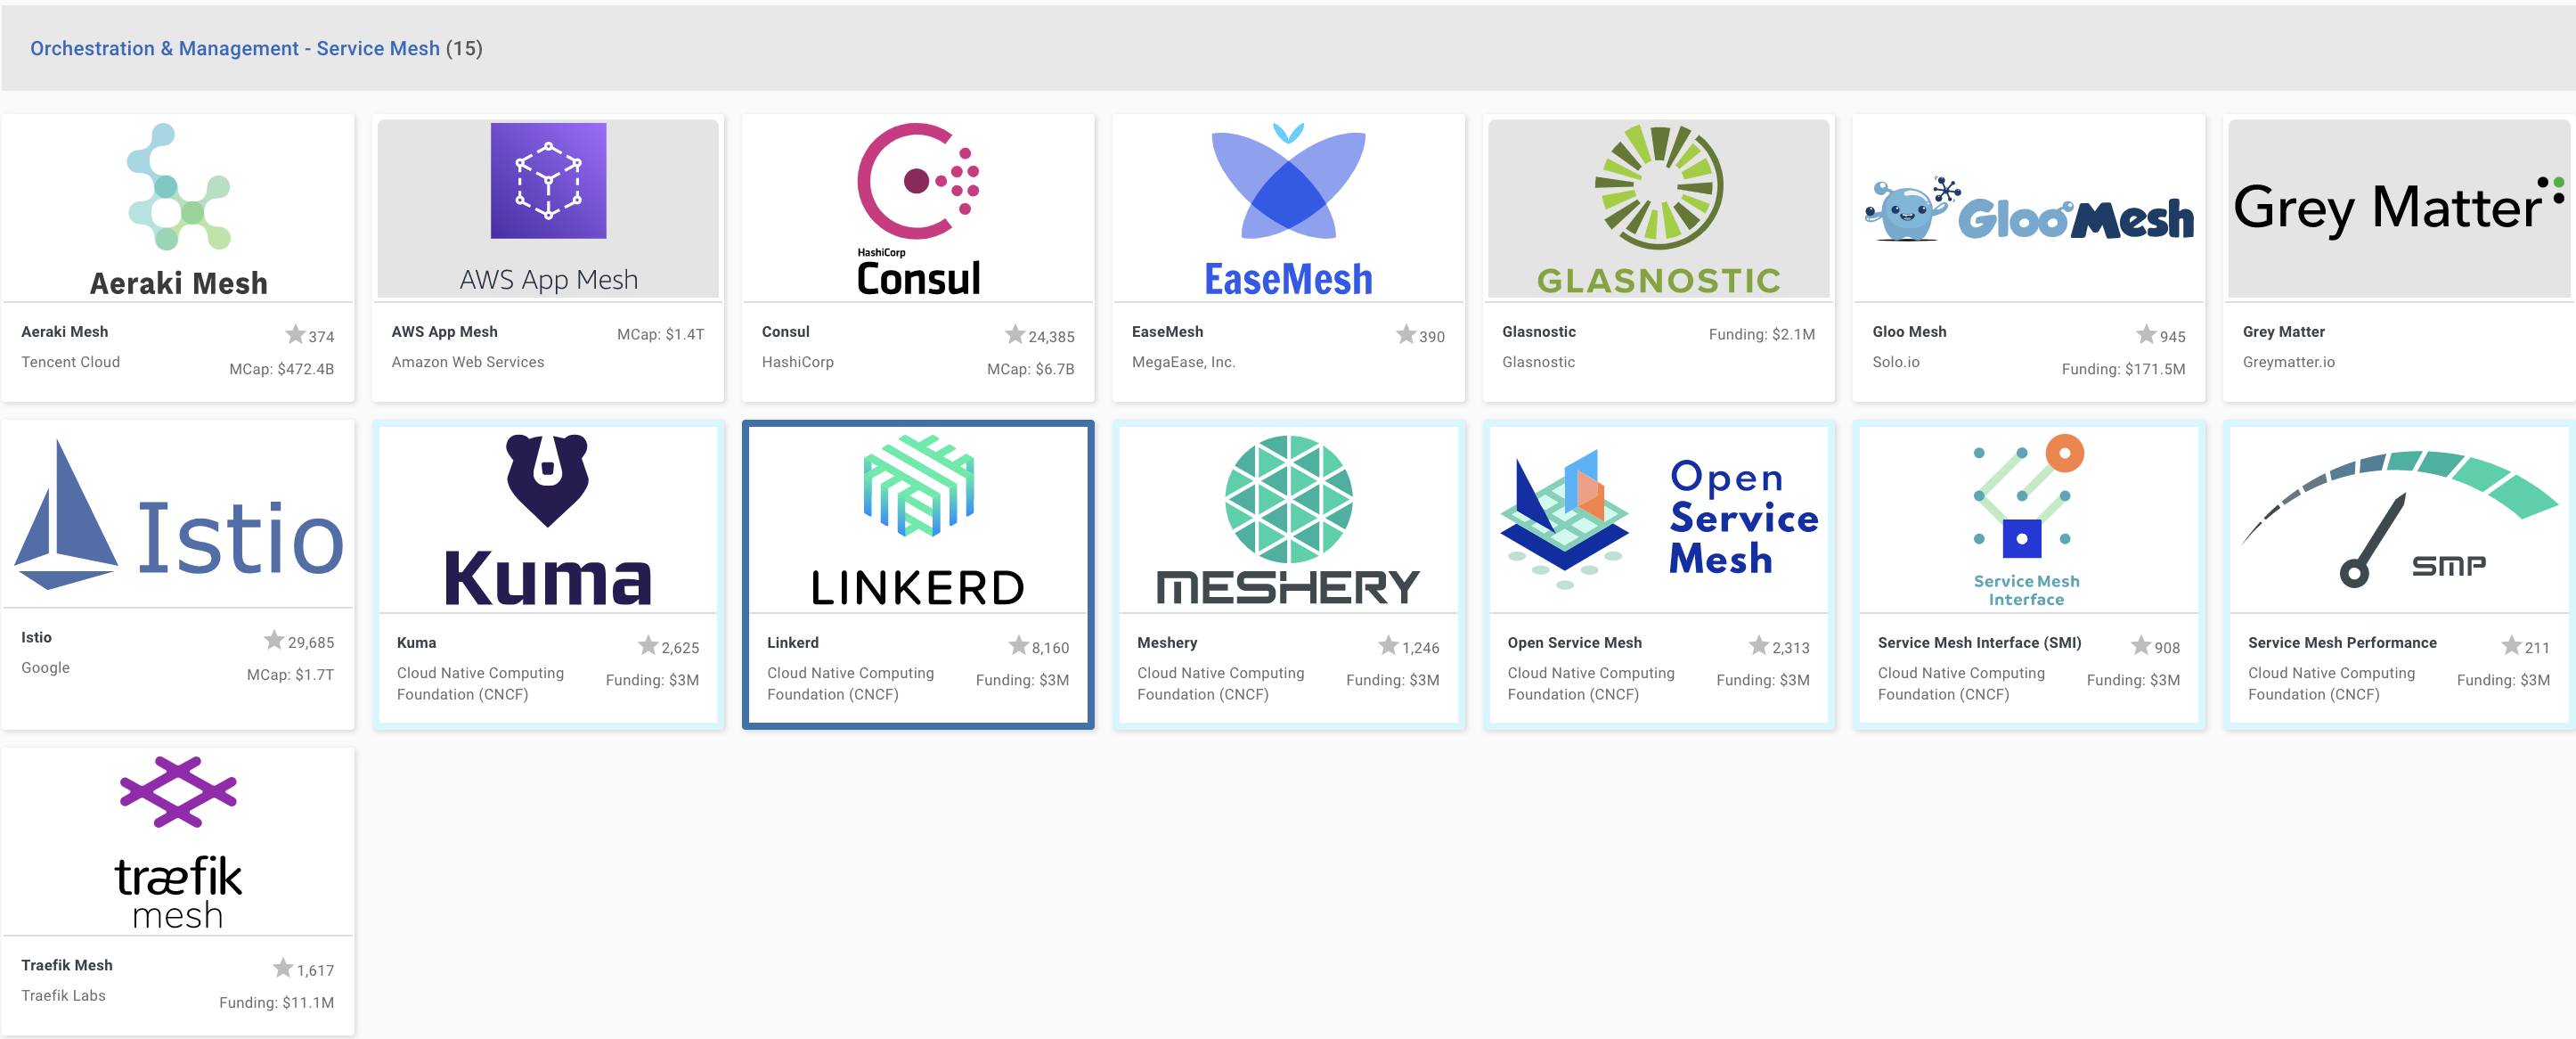
\includegraphics[width=0.9\linewidth]{3_systems_survey/figures/cncf-landscape-service-mesh}
    \caption{\gls{cncf} landscape of \gls{sm} technologies as of March 2022}
    \label{fig:cncf-landscape-sm}
\end{figure*}

% Conclude that there is a need for the review
% - Lack of formal (reiterate)
% - Industry interest
% - New approaches (proxyless, ebpf)
To justify a formal systematic survey, we have to evaluate the environment and related work. First, we have evaluated the existing formal literature in the field, as stated above, and concluded that this was lacking and unfit for the goals and research that we have in mind. Secondly, we evaluated the interest from within the community regarding the \gls{sm} technology. Our preliminary analysis showed that this was a sharp contrast against the interest from within the academic world. The field has an abundance of blog posts, talks, and the author of \gls{linkerd}, a popular \gls{sm} implementation, even went as far to call it \say{the world’s most over-hyped technology} \cite{service-mesh-hype}. Additionally, we found that the technology has received widespread adoption and interest from the industry, with a steady increase in production usage as indicated in surveys conducted by Red Hat \cite{rh-survey} and the \gls{cncf} \cite{cncf-survey-2020}. Finally, the very recent developments \cite{istio-merbridge, cilium-mesh} in the field (less than two months old at the time of writing), which fundamentally change the approach, provide  interesting takes to survey this field at this very moment. This all results in a justification for conducting the survey, and that the timing of it manages to capture an interesting, evolutionary shift within the field.


\section{Goals}
\label{sec:survey:goals}
% What are we trying to achieve in this survey
% - Bridge the gap between academia and industry
% - Gain insights into the current state-of-the-art-systems
% - Obtain knowledge about relative metrics and workloads 
% - ^> Is a stepping stone to the next chapter

% - Tie it all to the research question defined in the introduction

Before conducting a systematic systems survey, we first establish a set of goals which we will try to achieve in this work. This allows us to structure the research and adjust its methodologies based on the goals. The following list represents the formulated goals.

\begin{enumerate}[label=\textbf{G\arabic*}, leftmargin=3\parindent]
    \item \textbf{Bridge the gap between academia and industry.}
    \label{g-1}
    
    In the previous section (\cref{sec:survey:related-work}), we identified that there is a large gap between interest from academia and the industry. We identified that there is a lack of formal publications in the field, whereas preliminary exploration showed that this is in sharp contrast to the interest as expressed from the industry. This leads to this first goal, which is to close this gap and provide formal research in this emerging field.
    
    \item \textbf{Gain insight into the current state-of-the-art \gls{sm} systems.}
    \label{g-2}
    
    The second goal of this survey is to gain a clear understanding of the field and the current state-of-the-art \gls{sm} systems. We want to identify the systems that currently exist and identify their defining properties and characteristics.

    \item \textbf{Obtain knowledge about relevant performance metrics.}
    \label{g-3}
    
    Finally, we want to identify metrics that properly capture the performance implications of these systems. By examining these systems in detail, we want to obtain the metrics which are relevant in the application domain. 

\end{enumerate}

% - Tie it all to the research question defined in the introduction
% - Tie it to the general flow of the thesis as this provides a stepping stone to further chapters
The goals and their respective order in which they are  presented are closely tied to the general flow of research conducted within this thesis. We first established the gap between industry and academia in our previous work and formulated this thesis around the idea to close this \ref{g-1}. Furthermore, we apply best practices by conducting a survey of the field. This helps us to understand the field and allows us to examine the current state-of-the-art systems in detail \ref{g-2}. The data synthesis of this survey allows us to establish a framework to compare the existing and future \gls{sm} systems which might emerge. The results of this will be used to provide the answer to the research question \ref{rq-1} during our analysis. Additionally, the survey and resulting framework allows us to determine relevant metrics \ref{g-3}. This provides a stepping stone towards the following chapter, in which we design an instrument to compare the performance characteristics of these systems (\cref{chap:system-design}).
\section{Methodology}
\label{sec:survey:methodology}

% General intro of what is happening in this chapter
% - Systematic approach to a survey (reproducible)
% - Section structure
The following section covers the methodology that is used throughout the systematic systems review. The idea of the systematic approach is to make the results as presented in this chapter reproducible. This is done by extensively detailing the methodology used and explaining the decisions we had to take. We present the guidelines, data sources and steps taken to reach the dataset used in the data synthesis. 

The remainder of this section is structured as follows. First, in \cref{sec:survey:methodology:strategy} we identify and discuss methods and techniques commonly used in systems surveys. Secondly, in \cref{sec:survey:methodology:approach}, we combine the methods and techniques identified, and present the strategy that we used to approach this survey. Subsequently, we introduce the research protocol that we established to conduct the survey.




\subsection{Defining a Strategy}
\label{sec:survey:methodology:strategy}

% Introduction to strategy definition


There are many methods and techniques out there to find, select or synthesize the data for a survey. The methodology and technique used throughout such a survey ultimately dictates the form a survey takes on and influences the results it produces. It is important to identify, compare and choose such methods and techniques that fit the needs of our system-focussed survey. 

In this section, we will present the identified methods that we can use for a survey. For each method, we discuss their advantages and disadvantages and whether we will use them in some form within the survey.

\subsubsection{Unguided Techniques}
\label{sec:survey:methodology:strategy:unguided}

% Analysis of common survey methods
% - Unguided Methods
% - Unguided Search -> Initial dataset
% - Backward Snowballing -> Enhange datase


\textit{Unguided search} is the first technique that we have identified. This technique is commonly used to produce an initial dataset of relevant literature on the topic. This process requires the researcher to traverse various digital libraries equipped with relevant keywords to produce the dataset. Another commonly used technique that we have identified is \textit{backward snowballing}. This is another unguided method often used as a complementary technique to expand the dataset and is achieved by searching for related papers in the reference section. By combining these techniques, a researcher can create a literature review based on the generated dataset. However, both of the techniques are unguided, and therefore the process is not reproducible. Using such unguided techniques can result in entirely different datasets if the process is to be repeated by another researcher, and thus does not produce much scientific value. 

% Analysis of common survey methods
% - Guided Methods
% - SLR (Kitchenham) -> Planning, Conducting, Reporting
% - Petersen -> comparative analysis guidelines
\subsubsection{Systematic Approach}
\label{sec:survey:methodology:strategy:systematic}

% SLR
To prevent any form of bias to have an effect on the process and results of a survey, we have to establish and utilize a systematic approach. We have identified a state-of-the-art methodology which aims to create a systematic process which will be used to guide this survey. The works of Kitchenham and Charters \cite{Kitchenham2007} introduce a battle-tested and auditable set of guidelines for literature reviews aimed at software engineering researchers  with the goal of promoting reproducibility. The introduced \textit{\gls{slr}} methodology consists of three steps, planning the review, conducting the review and reporting the review. We decided to use these guidelines as a baseline for the survey, as it aligns with our goals and environment.

In addition to the guidelines introduced by the \gls{slr} methodology, we utilize the guidelines as introduced in the works of Petersen et al. \cite{Petersen2008, Petersen2015}. The authors introduce a set of guidelines and techniques which can be used to conduct a mapping study on a given topic. Among the guidelines and techniques, the authors introduce a method to perform comparative analysis. These guidelines and methods align with our needs and goals to compare \gls{sm} systems in the field as stated by the formulated research question \ref{rq-1}. 

% MLR method (Garousi)
% - MLR (Garousi) -> Inclusion of GL
\subsubsection{Inclusion of Grey Literature}
\label{sec:survey:methodology:strategy:gl}

% - Previous lit survey -> Lack of PL
% - 2019 Secondary survey -> Lack of PL
% - Most content from the industry is GL
One of the drawbacks of the \gls{slr} method is that it only concerns \gls{pl}, which consists of published peer-reviewed academic articles. In our previous work, in which we have conducted a systematic literature review on the \gls{k8s} ecosystem, we came to the conclusion that this field lacked published and peer-reviewed articles. Additionally, previous secondary studies on the field came to the same conclusion \cite{service-mesh-survey}. The lack of published (formal) literature in the field makes it impossible for us to conduct the research to an extent which satisfies our goals. This led us to explore additional forms of literature. \Gls{gl} is a form of literature that does not belong in the formal category, and can be in the form of blog posts, videos or white papers. Exploratory research has shown that inclusion of \gls{gl} can be beneficial to our research, as most of the literature is presented in such form by the industry.

% - Introduction to MLR
To maintain a systematic approach with the inclusion of \gls{gl}, we had to define or find additional guidelines that supported this requirement. We have identified the state-of-the-art method for conducting a survey which enabled the inclusion of \gls{gl}. The \gls{mlr} methodology as introduced by Garousi et al. \cite{Garousi2019} adapts and extends the \gls{slr} method from Kitchenham et al. so that it can include both forms of literature. 

% MLR checklist table
\begin{table*}[t]
\centering
\resizebox{\linewidth}{!}{ %< auto-adjusts font size to fill line
    \begin{tabular}{@{}lll@{}}
    \toprule
    \# & Question & Answer \\
    \midrule
    1 & Is the subject “complex” and not solvable by considering only the formal literature? & Yes \\
    2 & Is there a lack of volume or quality of evidence, or a lack of consensus of outcome measurement in the formal literature? & Yes \\
    3 & Is the contextual information important to the subject under study? & Yes \\
    4 & Is it the goal to validate or corroborate scientific outcomes with practical experiences? & Yes \\ 
    5 & Is it the goal to challenge assumptions or falsify results from practice using academic research or vice versa? & No \\ 
    6 & Would a synthesis of insights and evidence from the industrial and academic community be useful to one or even both communities? & Yes \\ 
    7 & Is there a large volume of practitioner sources indicating high practitioner interest in a topic? & Yes \\ 
    \bottomrule
    \end{tabular}
} %< \resizebox
\caption[Questionnaire to decide whether to include \gls{gl}. ]{Questionnaire from the works of Garoussi et al. \cite{Garousi2019}, which helps to decide whether to include \gls{gl} in a literature survey.}
\label{tab:mlr-checklist}
\end{table*}

% - MLR requriements checklist
Additionally, the authors have created a checklist which can be used to verify the need for inclusion of \gls{gl} within a survey. If one or more of the questions in the checklist is answered with a \say{yes}, it indicates that \gls{gl} can be beneficial to the survey. We answered the questions in the provided checklist and the results of this can be seen in \cref{tab:mlr-checklist}. These results reaffirmed our requirement for \gls{gl} throughout the survey and made us adapt the guidelines as described by the methodology.




\subsection{Our Approach to a Systematic Survey}
\label{sec:survey:methodology:approach}
%  Summarize entire approach and present figure that shows this
% - SLR Leeading
% - MLR -> inclusiong of GL
% - Petersen -> comparitive analysis

In the previous section (\cref{sec:survey:methodology:strategy}), we identified several methodologies and guidelines which we can use to conduct a survey. We explained why we have chosen some of these guidelines for our systems survey and how they could apply to our research goals. The resulting strategy can be seen in more detail in the form of a flow chart in  \cref{fig:survey-methodology}. This figure depicts two of the three stages in from the \gls{slr} methodology, namely the planning phase and the conducting phase. It also lists all the deliverables of this systems survey (\designref{D1} - \designref{D5}). 

Up to this point, we have discussed two steps of the planning phase. This first step of the planning phase \designref{P1}, consists of establishing a need for the survey, which we did in \cref{sec:survey:related-work}. Next, we established our goals \ref{g-1} - \ref{g-3} and research question \ref{rq-1} in \cref{sec:survey:goals} which relates to process \designref{P2}.




% Support findings based on some perspectives
\begin{figure}[!t]
    \centering
    
    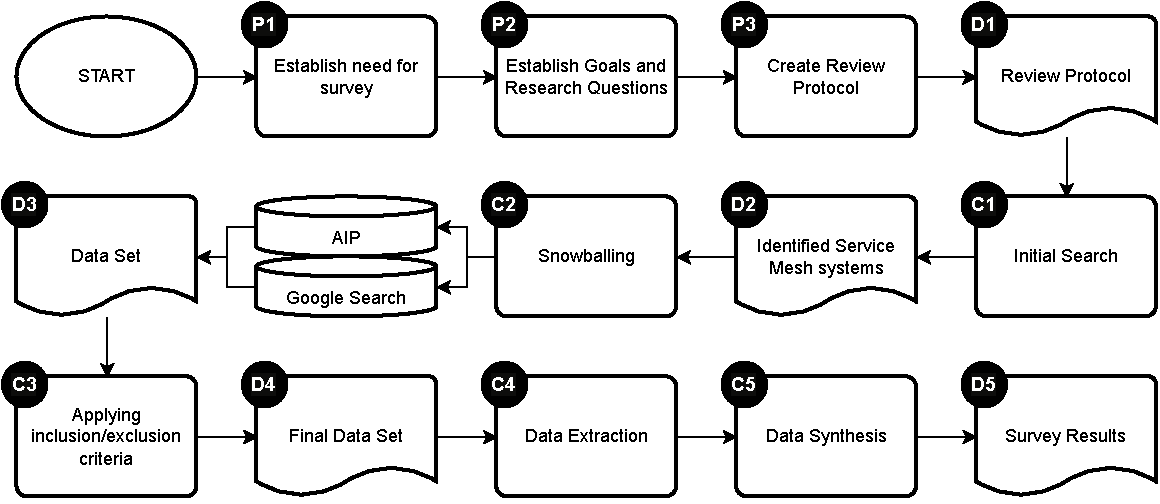
\includegraphics[width=\linewidth]{3_systems_survey/figures/survey-methodology}

    \caption{System Survey approach.}
    \label{fig:survey-methodology}
\end{figure}




% % SLR Plannign phase
% % 1. Investigate need (rel. work)
% % 2. Objective of this research
% % 3. Formulate RQ.
% \subsection{Planning}
% \label{sec:survey:methodology:planning}

% \todo{Fix planning section}

% In line with the guidelines as proposed in the \gls{slr} methodology, we first conducted a planning stage. During this stage we have analysed relevant work and the need for a review as discussed in \cref{sec:survey:related-work}. After this, we formulated the goal and related research question of this survey as seen in \cref{sec:survey:goals}. The goal of this systems survey is to uncover the existing \gls{sm} systems in the landscape and provide an overview of characteristics that they have. By creating a data synthesis of the literature that we are able to find on this topic, we can produce a general framework to contain these systems. This is a stepping stone for the research that is conducted in the later chapters, in which we examine and evaluate the characteristics and performance properties of these systems in more detail. 



% SLR - Review Protocol
\subsection{Review Protocol}
\label{sec:survey:methodology:review-protocol}

% Review protocol consists of
% - Background, the rationale for the survey -> Goals
% - Research Questions that we intend to answer


% PL & GL
% - Search Strategy
% - Selection Criteria
% - Selection Procedures
% - Data Extraction



The review protocol is a fundamental aspect of the \gls{slr} methodology, it specifies the methods used to conduct the systems review in this thesis. A pre-defined protocol is required to reduce the possibility of any bias. Establishing the review protocol is part of our approach as specified in \cref{fig:survey-methodology} and depicts the process \designref{P3}.

In the remainder of this section, we introduce the components that establish the research protocol. In \cref{sec:survey:methodology:review-protocol:search-strategy}, we introduce the search strategy which is used to search for the relevant literature. In \cref{sec:survey:methodology:review-protocol:selection-criteria}, we establish the selection criteria which are used to filter the dataset which we obtained through the research strategy. Finally, in \cref{sec:survey:methodology:review-protocol:data-extraction}, we describe the methods used to extract and synthesize the data.



\subsubsection{Search Strategy}
\label{sec:survey:methodology:review-protocol:search-strategy}
% - Data Sources
% - Queries

To create a reproducible data set, we have to establish a search strategy which we use to obtain literature on the topic. The search strategy differs based on the type of literature, where different requirements apply for \gls{pl} and \gls{gl}.


% Data sources
% - AIP
% - Digital Libraries (DBLP, Aminer, Semantic Scholar)
% - Only established, well respected conferences
The first component that makes up the search strategy is related to the data sources. The Atlarge  team\footnote{\url{https://atlarge-research.com/}} has identified several digital libraries which are well established and which contain the leading publications in the field of distributed systems. Additionally, years of experience in the field led to the creation of a list of established and well-respected conferences. This consolidated knowledge led to the development of a software instrument \gls{aip}. This instrument is used to generate the initial dataset of \gls{pl} for this survey and query it. To establish a dataset of \gls{gl} in this survey, we use Google Search to identify relevant literature.

The second component of the search strategy is related to the search technique. Since the goal of this survey to compare state-of-the-art \gls{sm} systems, we first have to identify said systems. To achieve that, we first conducted exploratory research in the field. To reduce bias in this process, we first used the single identified secondary study \cite{service-mesh-survey} to obtain an initial set of \gls{sm} systems. After this, we identified the \gls{sm} systems that were part of official \gls{cncf} projects\footnote{\url{https://landscape.cncf.io/card-mode?category=service-mesh&grouping=category}}, as they have proven to be an authoritative entity in the field as discussed in \cref{sec:background:cncf}. This list was then complemented by results obtained from \gls{gl} using generic search queries. 


The final component of the search strategy is related to the search queries that we use to establish the resulting dataset. To find and identify the current state-of-the-art \gls{sm} systems, we used generic terms as described above. After this, we utilized a snowballing method in which we based the search queries on the identified systems. The final list of search queries used can be seen in \cref{tab:search-queries}. Queries \textbf{Q1} and \textbf{Q2} represent the queries used to obtain and expand the list of identified \gls{sm} systems, while \textbf{Q3} indicates the system-specific queries that were used. 

\begin{table}[t]
\centering
% \resizebox{\linewidth}{!}{ %< auto-adjusts font size to fill line
    \begin{tabularx}{\linewidth}{lXl}
    \toprule
    \# & Query & Search Strategy \\
    
    % Initial Search Queries
    \midrule
    \textbf{Q1} & Service Mesh & Initial Search \\
    \textbf{Q2} & Service Mesh Implementation & Initial Search \\

    % Queries Based on identified SM systems
    \midrule
    \textbf{Q3} & \textit{Identified Service Mesh Implementation} & Snowballing  \\
    
    \bottomrule
    \end{tabularx}
% } %< \resizebox
\caption{Search queries established in the review protocol.}
\label{tab:search-queries}
\end{table}

% \begin{table}[t]
% \centering
% % \resizebox{\linewidth}{!}{ %< auto-adjusts font size to fill line
%     \begin{tabular}{@{}lll@{}}
%     \toprule
%     \# & Query & Search Strategy \\
    
%     % Initial Search Queries
%     \midrule
%     \textbf{Q1} & Service Mesh & Initial Search \\
%     \textbf{Q2} & Service Mesh Implementation & Initial Search \\

%     % Queries Based on identified SM systems
%     \midrule
%     \textbf{Q3} & \textit{Identified Service Mesh Implementation} & Snowballing  \\
    
%     \bottomrule
%     \end{tabular}
% % } %< \resizebox
% \caption{Search queries established in the review protocol.}
% \label{tab:search-queries}
% \end{table}



\subsubsection{Selection Criteria}
\label{sec:survey:methodology:review-protocol:selection-criteria}
% Seperate Criteria for PL and GL
% Introduce the checklist and how it works
% display PL and GL checklist
Since we have decided to also include \gls{gl} in our survey, we decided to establish two sets of selection criteria since they are vastly different in terms of content and medium. For both types of literature, we establish a checklist. In this checklist, we define the guidelines that we use to either include or exclude a data point. Guidelines prefixed with a checkmark (\cmark) symbol indicate a reason to include a publication in the research, whereas the cross (\xmark) symbol indicates a reason for exclusion. 

The following checklist (\cref{list:checklist:pl}) contains a set of selection criteria that applies to the \gls{pl} that is obtained through the search process. For this, we apply a set of generic criteria in order to 

In addition to the search queries, we used a filter to filter out any results before 2014 since that the initial release date of \gls{k8s} \cite{kubernetes-overview}. This limits the results based on the scope of this research, which provides a focus on \gls{sm} systems in the \gls{k8s} ecosystem.

\begin{itemize}
    \item[(\cmark)] Publications that are written in English.
    \item[(\cmark)] Publications introducing novel concepts.
    \item[(\cmark)] Publications that focus on architectural problems and solutions.
    \item[(\cmark)] Publications performing performance analysis studies.
    
    \item[(\xmark)] Publications before 2014. 
    \item[(\xmark)] Publications that do not have \gls{sm} systems as the primary subject in the research. 
    \item[(\xmark)] Secondary or tertiary studies regarding \gls{sm} systems.
    \item[(\xmark)] Publications that are not full-text (e.g., small snippets or as part of a demo).
    
    \label{list:checklist:pl}
\end{itemize}


The following checklist (\cref{list:checklist:gl}) contains a set of selection criteria that applies to the \gls{gl} that is obtained through the search process. For this form of literature we had to establish a set of rigorous guidelines since it can otherwise result in numerous data entries or lead to a biased set of results. 

\begin{itemize}
    \item[(\cmark)] Publications that are written in English.
    \item[(\cmark)] Publications introducing novel concepts.
    \item[(\cmark)] Publications originating from well established and known organizations (e.g. \gls{cncf}, Google, Red Hat, etc.).
    \item[(\cmark)] Publications that supply official vendor or platform documentation.
    \item[(\cmark)] Publications in the form of blog posts from organizations or authorities in the field.
    \item[(\cmark)] Publications in the form of videos from talks or conferences related to the field.
    \item[(\cmark)] Source code repositories of open-source \gls{sm} systems (e.g., a GitHub repository).
    
    \item[(\xmark)] Publications in which we cannot validate the authority of an author (e.g., anonymous posts, or posts by someone not established in the field). 
    \item[(\xmark)] Publications which do not provide any novelty for the survey (e.g., tutorials on the technologies). 
    \item[(\xmark)] Publications that are not full-text (e.g., small snippets, parts of a demo or short social media excerpts such as tweets).
    
    \label{list:checklist:gl}
\end{itemize}


\subsubsection{Data Extraction}
\label{sec:survey:methodology:review-protocol:data-extraction}
% What kind of information is relevant to us
% Compare systems
% Observability
% Resilience
% Proxy Characteristics
% Protocol Support
% Security
% Meta


Once we have established a final dataset by filtering the dataset based on the selection criteria, we can start the data synthesis process. To achieve this, we first have to establish a set of data extraction guidelines. These guidelines have to be in line with the goals which of this survey. Since we want to compare  state-of-the-art \gls{sm} systems, we have to identify the key characteristics and properties  of such systems. Through the preliminary research conducted on the field, we understand the fundamentals of a \gls{sm} system and have identified the challenges it tries to solve. With this in mind, we try to identify and synthesize the data based on key areas.


% Observability
% Resilience
% Proxy Characteristics
% Protocol Support
% Security
% Meta
First off, we try to compare these systems based on their architectural approach. With this take, we can identify and compare \gls{sm} systems based on their design decisions, such as their control and data plane components. Secondly, we take a functional approach to synthesize these systems. By identifying sets of functionality, we can evaluate and compare these systems on domain-specific functionalities such as their observability, security, or resiliency characteristics. Furthermore, we take a meta analytical approach to these systems. With this, we try to establish certain aspects such as the number of users the system has, the development activity on the project, whether a project is open-source or not and the maturity of the system.
\section{Results}
\label{sec:survey:results}

% General intro of what is happening in this chapter
% - Identified Service Mesh Systems
% - Identified requirements
% - Comparison Framework

In this section, we present the results from the systems survey as deliverable \designref{D5}. First, we present the identified \gls{sm} systems in \cref{sec:survey:results:sm-systems}. Furthermore, in \cref{sec:survey:results:sm-requirements} we introduce functional and non-functional requirements which we use to differentiate \gls{sm} systems. Finally, in \cref{sec:survey:results:sm-framework} we present a comparison framework for state-of-the-art \gls{sm} systems, in which we compare the identified systems.


% Identified SM systems
% - 12 Systems
% - Why we dont include managed istio services
\subsection{State-of-the-art Service Mesh Systems}
\label{sec:survey:results:sm-systems}

During the initial phase of the systems survey, we set out to identify existing \gls{sm} systems with our initial search strategy (\textbf{Q1} \& \textbf{Q2} in \cref{tab:search-queries}). During this phase, we identified 14 different \gls{sm} systems, which can be seen in \cref{tab:sm-implementations}, which represents deliverable \designref{D2}. By identifying these systems, we could run targeted queries on these them, which enabled us to dive deeper into their individual architectures.

% SM Implementations table
\begin{table*}[t]
\centering
\resizebox{\linewidth}{!}{ %< auto-adjusts font size to fill line
    \begin{tabular}{@{}lll@{}}
    \toprule
    ID & Service Mesh & Vendor Page \\
    
    % Included SM implementations
    \midrule
    \textbf{SM1}\label{sm1} & AWS App Meshh & \url{https://aws.amazon.com/app-mesh/} \\
    \textbf{SM2}\label{sm2} & Cilium & \url{https://cilium.io/} \\
    \textbf{SM3}\label{sm3} & Consul & \url{https://www.consul.io/} \\
    \textbf{SM4}\label{sm4} & Ease Mesh & \url{https://megaease.com/easemesh/} \\
    \textbf{SM5}\label{sm5} & Istio & \url{https://istio.io/} \\
    \textbf{SM6}\label{sm6} & Kuma & \url{https://kuma.io/} \\
    \textbf{SM7}\label{sm7} & Linkerd2 & \url{https://linkerd.io/} \\
    \textbf{SM8}\label{sm8} & Nginx Service Mesh & \url{https://www.nginx.com/products/nginx-service-mesh} \\
    \textbf{SM9}\label{sm9} & Open Service Mesh & \url{https://openservicemesh.io/} \\
    \textbf{SM10}\label{sm10} & Traefik Mesh & \url{https://traefik.io/traefik-mesh/} \\
    
    % Excluded SM implementations
    \midrule
    \textbf{-} & Alibaba Cloud Service Mesh & \url{https://www.alibabacloud.com/product/servicemesh} \\
    \textbf{-} & Aspen Mesh & \url{https://aspenmesh.io/} \\
    \textbf{-} & Citrix ADC & \url{https://www.citrix.com/nl-nl/products/citrix-adc/} \\
    \textbf{-} & Linkerd & \url{https://linkerd.io/} \\
    \bottomrule
    \end{tabular}
} %< \resizebox
\caption[Identified \gls{sm}.]{Identified \gls{sm} systems and their respective vendor pages. The \gls{sm} systems with an ID as indicated in the table, will be used and referred to throughout the rest of the system survey.}
\label{tab:sm-implementations}
\end{table*}

However, some systems in the list will be excluded from the rest of the work presented in this thesis. In particular, \textit{Alibaba Cloud Service Mesh},  \textit{Aspen Mesh}, \textit{Citrix ADC}, and \textit{Linkerd} are excluded. The first two systems are managed, closed-source service offerings of the popular \textit{Istio} \gls{sm}. The third system, has the option to utilize  \textit{Istio} to construct a \gls{sm}. We excluded these systems, as they provide no unique capabilities, are presented in the form of black box software and additionally has a financial cost attached to it. Finally, the last of the excluded systems mentioned, is superseded by \textit{Linkerd2} and is discontinued. 

% Identified SM systems
\subsection{Identified Requirements}
\label{sec:survey:results:sm-requirements}

To compare existing \gls{sm} systems, we have to introduce a set of requirements to compare them on. We do this in the form of \textit{Functional Requirements} and \textit{Non-Functional Requirements}. The former set of requirements describe the functions and characteristics of a system, such as the features and capabilities a specific system has. The latter, however, take a more general approach to describing the systems on its behaviour.

% Most important aspects of a service mesh
\subsubsection{Functional Requirements}
\label{sec:survey:results:sm-requirements:fr}

In this section, we introduce a list of six \textit{Functional Requirements} (\ref{fr-1} - \ref{fr-4}). We derived these requirements from the core functionalities of \gls{sm} systems. For each of the defined requirements, we provide a brief description of what the requirement entails and how we extract the information from the identified systems to measure this.


\begin{enumerate}[label=\textbf{FR\arabic*}, leftmargin=3\parindent]
    \item \textbf{Observability Capabilities}
    \label{fr-1}
    Indicates whether the system supports a wide variety of observability capabilities. Observability characteristics range from capturing metrics, to monitoring and tracing. To determine this, we have established a list of capabilities on which we compare these systems.
    
    \item \textbf{Security Capabilities}
    \label{fr-2}
    Indicates whether the system supports common security capabilities. To determine this, we first established a list of common security features, on which we compare the individual systems.
    
    \item \textbf{Resilience Capabilities}
    \label{fr-3}
    Indicates whether the system supports a wide variety of reliability characteristics. \Gls{sm} systems can improve the reliability of service-to-service communications in a system. To determine the capabilities of an individual system, we established a list of common reliability characteristics and compared the individual systems to these capabilities.
    
    \item \textbf{Support for Multiple Deployment Models}
    \label{fr-4}
    Indicates whether the system supports multiple deployment models. The most common scenario is to have a single cluster and a single service mesh. However, situations might exist where a topology consists of multiple clusters or multiple \glspl{sm} to provide for extra isolation, for example. We compare the identified systems to check for support on this characteristic.
\end{enumerate}


\subsubsection{Non-Functional Requirements}
\label{sec:survey:results:sm-requirements:nfr}

In this section, we introduce a list of six \textit{Non-Functional Requirements} (\ref{nfr-1} - \ref{nfr-5}). We established this list to provide for a general overview of the \gls{sm} systems. For each of the defined requirements, we provide a brief description of what the requirement entails and how we extract the information from the identified systems to measure this.



\begin{enumerate}[label=\textbf{NFR\arabic*}, leftmargin=3\parindent]
    \item \textbf{Application Protocol Support}
    \label{nfr-1}
    Service proxies can be aware of application level protocols to allow application level routing and rich metrics. This requirement indicates whether a \gls{sm} system supports a wide variety of application level protocols. To determine this, we established a list of common service-to-service protocols and also identified additional application level protocol support for each of the identified systems. The requirement is only fully satisfied if, in addition to the commonly listed protocols, it supports additional application level protocols.

    \item \textbf{Open-source}
    \label{nfr-2}
    Indicates whether a \gls{sm} system is available in the form of open-source software. To determine this, we identified source code repositories for the individual \gls{sm} systems if they existed.
    
    \item \textbf{Thoroughly Documented}
    \label{nfr-3}
    Indicates whether the system is extensively documented. This is determined by examining the vendor documentation on the system. The requirement is not satisfied if there is no vendor documentation partially satisfied if there is some form of vendor documentation, but not extensive or up to date, and fully satisfied if there is extensive and well-written documentation on the system.
    
    \item \textbf{Cloud Native Computing Foundation Project}
    \label{nfr-4}
    
    Indicates whether a \gls{sm} system is recognized as an official \gls{cncf} project and if so, which level of maturity it currently has. The \gls{cncf} defines three levels of maturity for each of its projects and imposes certain guidelines to achieve a new level of maturity \cite{cncf-project-graduation-criteria}. The projects and their levels ranging from \textit{sandbox} to \textit{incubating} to \textit{graduating} can be found on their website \footnote{\url{https://landscape.cncf.io/card-mode?category=service-mesh&grouping=category}} and can indicate the maturity of a project. The requirement is not satisfied if it is not a formal project, partially satisfied if it is in the \textit{sandbox} or \textit{incubating} stage, and fully satisfied if it is a \textit{graduated} project.


    \item \textbf{Community Recognition}
    \label{nfr-5}
    
    Indicates the recognition as per the community of users. We determine this by looking at various metrics and surveys regarding the usage of individual systems. For example, with open-source projects, we use community-related metrics such as GitHub stars. The requirement is partially satisfied if it has more than $10.000$ GitHub stars or more than 10 percent usage in production, according to the \gls{cncf} survey conducted in 2021 \cite{cncf-survey-2021}. To fully satisfy this requirement, the project needs more than $20.000$ GitHub stars or has more than 25 percent usage in production. 
\end{enumerate}



\subsection{Comparing Service Mesh Systems}
\label{sec:survey:results:comparison}

In this section, we present the results of the data synthesis based on the identified Functional and Non-Functional Requirements (\cref{sec:survey:results:sm-requirements:fr}, \cref{sec:survey:results:sm-requirements:nfr}). First, in \cref{sec:survey:results:comparison:proxy}, we compare the \gls{sm} systems on their service-to-service proxy. Secondly, in \cref{sec:survey:results:comparison:observability}, we compare the systems based on their observability capabilities. After that, in \cref{sec:survey:results:comparison:security}, we compare the systems on the most common security features. Following that, in \cref{sec:survey:results:comparison:resilience}, we evaluate the resiliency features of the systems. Finally, in \cref{sec:survey:results:comparison:nfr}, we show the obtained non-functional requirements regarding the systems. These results provide a stepping stone to the analysis in \cref{sec:survey:analysis}.

\subsubsection{Proxy Systems}
\label{sec:survey:results:comparison:proxy}
% Custom vs Common proxy
% Architectural Style
% Traffic Proxy

\begin{table*}[t]
\centering
\resizebox{\linewidth}{!}{ %< auto-adjusts font size to fill line
\begin{tabular}{ll|llcc}


\toprule

% HEADER 1
\multicolumn{2}{c|} {\textbf{Service Mesh}} &
\multicolumn{4}{c} {\textbf{Service Proxy Capbilities}}  \\

% HEADER 2
ID &
Name &
Service Proxy &
Proxy Architecture &
Proxy TCP &
Proxy UDP \\


\midrule


\textbf{SM1} &
AWS App Mesh  & 
Envoy & 
Per-Service & 
\cmark & 
\cmark \\


\textbf{SM2} &
Cilium  & 
Cilium (\gls{ebpf}) & 
In-Kernel & 
\cmark & 
\cmark \\


\textbf{SM3} &
Consul  & 
Envoy* & 
Per-Service & 
\cmark & 
\cmark \\


\textbf{SM4}&
Ease Mesh & 
Easegress & 
Per-Service & 
\cmark & 
\xmark \\


\textbf{SM5} &
Istio & 
Envoy & 
Per-Service & 
\cmark & 
\cmark \\


\textbf{SM6} &
Kuma & 
Envoy & 
Per-Service & 
\cmark & 
\cmark \\


\textbf{SM7} &
Linkerd2 & 
Linkerd2 Proxy & 
Per-Service & 
\cmark & 
\xmark \\


\textbf{SM8} &
Nginx Service Mesh & 
NGINX Plus & 
Per-Service & 
\cmark & 
\cmark \\


\textbf{SM9} &
Open Service Mesh  & 
Envoy & 
Per-Service & 
\cmark & 
\cmark \\


\textbf{SM10} &
Traefik Mesh &
Traefik Proxy & 
Per-Node & 
\cmark & 
\cmark \\


\bottomrule
\end{tabular}

} %< \resizebox
\caption
[Comparing the proxy capabilities of service mesh systems.]
{Comparing the proxy capabilities of identified service mesh systems. \\

\textit{Service Proxy} indicates the type of proxy component used, as this is considered an implementation detail of the service mesh architecture (see background \cref{sec:background:service-mesh}). \\
\textit{Proxy Architecture} refers to the manner in which the proxy is introduced within the system (see \cref{sec:survey:analysis:architectures}). \\
\textit{Proxy TCP} and \textit{Proxy UDP} support features indicate whether the \textit{Service Proxy} can proxy this type of traffic or whether it just forwards the type of traffic. 

\cmark: Indicates that the feature is supported. \\
\xmark: Indicates that the feature is no supported. \\
*: Can be interchanged for other service proxies.
}
\label{tab:result-proxy}
\end{table*}







% \begin{table*}[t]
% \centering
% \resizebox{\linewidth}{!}{ %< auto-adjusts font size to fill line
% \begin{tabular}{l|llll}
% \toprule
% Service Mesh       & Service Proxy  & Proxy Architecture & Proxy TCP & Proxy UDP \\
% \midrule
% AWS App Mesh       & Envoy          & Per-Service        & Yes       & Yes       \\
% Cilium             & Cilium eBPF    & Kernel (eBPF)      & Yes       & Yes       \\
% Consul             & Envoy*         & Per-Service        & Yes       & Yes       \\
% Ease Mesh          & Easegress      & Per-Service        & Yes       & No        \\
% Istio              & Envoy          & Per-Service        & Yes       & Yes       \\
% Kuma               & Envoy          & Per-Service        & Yes       & Yes       \\
% Linkerd2           & Linkerd2 Proxy & Per-Service        & Yes       & No        \\
% Nginx Service Mesh & NGINX Plus     & Per-Service        & Yes       & Yes       \\
% Open Service Mesh  & Envoy          & Per-Service        & Yes       & Yes       \\
% Traefik Mesh       & Treafik Proxy  & Per-Node           & Yes       & Yes       \\
% \bottomrule
% \end{tabular}

% } %< \resizebox
% \caption
% [Comparing the service-to-service proxy mechanisms of service mesh systems.]
% {Comparing the service-to-service proxy mechanisms of service mesh systems.

% *: Can be interchanged for other service proxies.
% }
% \label{tab:result-proxy}
% \end{table*}



First off, we compared the service-to-service proxy mechanisms of the identified \gls{sm} systems. At the core of a \gls{sm} system lies the service-proxy, it serves as the data-plane of the system and has a huge impact on the flow of traffic. The result of this comparison can be seen in \cref{tab:result-proxy}. While some \gls{sm} systems have their own custom service proxy, such as \textit{Linkerd2}, others utilize popular open-source proxy implementations such as \textit{Envoy}. Not all service proxies work and behave the same, the architecture of a proxy has a major impact on the traffic flow of a \gls{sm} system. During this survey, we have identified three different types of proxy architectures. First off, we identified a per-service proxy, such as used by most of the identified service proxies. This means that every service gets its own service proxy, and thus the number of proxies linearly scales with the number of services. The second architectural style identified is a per-node proxy, this is used by the \textit{Traefik Proxy}. This means that there is a single proxy per node, and that all services running on a node use that same proxy. The third and final architectural style identified also makes use of a single proxy per node but manages the traffic in the kernel space using \gls{ebpf}. Furthermore, we identified for each of the proxy systems if it was able to proxy TCP and UDP traffic. Being able to proxy TCP and/or UDP traffic means that the system will intercept any traffic of that type, and proxy it to the appropriate destinations. \Gls{sm} systems without UDP traffic proxy support can still have UDP traffic in their system, however, with the traffic not passing through the proxy it will provide none of the features that a \gls{sm} traditionally provides such as observability, security and resilience.


\subsubsection{Observability}
\label{sec:survey:results:comparison:observability}
% Metics system -> Nearly all prometheus
% Monitoring system -> Nearly all grafana
% Tracinf Support -> Jaeger > Zipkin > Open Standard
% Additional Dashboard -> Some have, e.g. custom topology inspection

\begin{table*}[t]
\centering
\resizebox{\linewidth}{!}{ %< auto-adjusts font size to fill line
\begin{tabular}{l|lllll}
\toprule
Service Mesh       & Metrics        & Monitoring     & Tracing                     & Dashboard \\
\midrule
AWS App Mesh       & AWS CloudWatch & AWS CloudWatch & AWS CloudWatch              & AWS X-Ray \\
Cilium             & Prometheus     & Grafana        & Jaeger, Open Telemetry      & Hubble    \\
Consul             & Prometheus     & Grafana        & Jaeger, Zipkin, OpenTracing & Consul UI \\
Ease Mesh          & Ease Monitor   & Ease Monitor   & OpenTracing                 & No        \\
Istio              & Prometheus     & Grafana        & Jaeger, Zipkin              & Kiali     \\
Kuma               & Prometheus     & Grafana        & Jaeger, Zipkin              & Yes       \\
Linkerd2           & Prometheus     & Grafana        & Open Telemetry              & Yes       \\
Nginx Service Mesh & Prometheus     & Grafana        & Jaeger                      & No        \\
Open Service Mesh  & Prometheus     & Grafana        & Jaeger                      & No        \\
Traefik Mesh       & Prometheus     & Grafana        & Jaeger                      & No        \\
\bottomrule
\end{tabular}
} %< \resizebox
\caption{Comparing the observability capabilities of identified service mesh systems.}
\label{tab:result-observability}
\end{table*}



Observability is a key feature and reason to use a \gls{sm}. The proxying of service-to-service communications allows systems to implement per-service metrics such as latencies, request volumes and error rates. We compared the identified \gls{sm} systems on key observability requirements, and the results of that can be seen in \cref{tab:result-observability}. First off, we identified the way in which the systems report metrics. Most of the identified systems made use of \textit{Prometheus}, a popular open-source time-series metric aggregator.  Furthermore, we compared the ways the systems enabled monitoring. Once again, \gls{sm} implementations resort to the same solution, this time in the form of \textit{Grafana}, a monitoring and observability platform. Tracing support, on the other hand, showed more variability. Most of the identified systems support \textit{Jaeger}, an open-source distributed tracing system. \textit{Zipkin} was another popular system with support, and some systems even supported open standards such as \textit{Open Telemetry}, allowing for any tracing system that supports that standard. Some \gls{sm} systems come with a bundled dashboard or have popular open-source extensions which enable this. These dashboards provide additional domain specific insights, such as provide graph tools to visualize the service mesh traffic topology. 

\subsubsection{Security}
\label{sec:survey:results:comparison:security}
% All services support MTLS (except Traefik)
% All services support S2S Authz (except Traefik)

\begin{table*}[t]
\centering
% \resizebox{\linewidth}{!}{ %< auto-adjusts font size to fill line

\begin{tabular}{ll|cc}


\toprule

% HEADER 1
\multicolumn{2}{c|} {\textbf{Service Mesh}} &
\multicolumn{2}{c} {\textbf{Security Capbilities}}  \\

% HEADER 2
ID &
Name &
Mutual TLS &
S2S Auth. Policies \\


\midrule


\textbf{SM1} &
AWS App Mesh  & 
\cmark  &
\cmark  \\

\textbf{SM2} &
Cilium  & 
\cmark  & 
\cmark \\


\textbf{SM3} &
Consul  & 
\cmark  & 
\cmark   \\


\textbf{SM4}&
Ease Mesh & 
\cmark  & 
\cmark \\


\textbf{SM5} &
Istio & 
\cmark  & 
\cmark   \\


\textbf{SM6} &
Kuma & 
\cmark  & 
\cmark   \\


\textbf{SM7} &
Linkerd2 & 
\cmark  & 
\cmark \\


\textbf{SM8} &
Nginx Service Mesh & 
\cmark & 
\cmark \\


\textbf{SM9} &
Open Service Mesh  & 
\cmark  & 
\cmark \\


\textbf{SM10} &
Traefik Mesh &
\xmark  & 
\xmark \\


\bottomrule
\end{tabular}
% } %< \resizebox

\caption[Comparing service mesh security capabilities]
{Comparing the security capabilities of identified service mesh systems.

\textit{Mutual TLS} indicates if the \gls{sm} system supports TLS authentications, which enables encrypted communications between service proxies. \\
\textit{S2S Auth. Policies} (Service-to-service authorization policies) indicate whether the \gls{sm} system supports advanced  authorization policies which enables the operator to grant or deny permissions to services to communicate with given entities (such as other services). \\

\cmark: Indicates that the feature is supported. \\
\xmark:  Indicates that the feature is no supported. }
\label{tab:result-security}
\end{table*}



Additional security is a feature that a \gls{sm} can provide. We compared the identified systems on the most common security characteristics a \gls{sm} can provide. The result of this can be seen in \cref{tab:result-security}. First, we identified if a \gls{sm} system can provide mutual TLS with little to no additional effort. This means that any service-to-service traffic is then encrypted and potential intruders in a network cannot inspect or intercept that traffic. All the systems, except \textit{Traefik Mesh}, support automatic mutual TLS encryption. Additionally, we compared the service-to-service authorization capabilities of these systems. This enables fine-grained control of access between services and users. Once again, all the systems, except \textit{Traefik Mesh}, have some form of authorization policies.

\subsubsection{Resilience}
\label{sec:survey:results:comparison:resilience}


\begin{table*}[t]
\centering
\resizebox{\linewidth}{!}{ %< auto-adjusts font size to fill line
\begin{tabular}{ll|cccccc}


\toprule

% HEADER 1
\multicolumn{2}{c|} {\textbf{Service Mesh}} &
\multicolumn{6}{c} {\textbf{Resiliency Capbilities}}  \\

% HEADER 2
ID &
Name &
Retry Funcionality &
Timeout Settings &
Rate Limiting &
Circuit Breaking &
Fault Injection &
Delay Injection \\


\midrule

\textbf{SM1} &
AWS App Mesh  & 
\cmark &
\cmark &
\xmark &
\cmark &
\xmark &
\xmark \\


\textbf{SM2} &
Cilium  & 
\cmark &
\cmark &
\cmark &
\cmark &
\cmark &
\cmark \\


\textbf{SM3} &
Consul  & 
\cmark &
\cmark &
\cmark &
\cmark &
\xmark &
\cmark\\


\textbf{SM4}&
Ease Mesh & 
\cmark &
\cmark &
\cmark &
\cmark &
\xmark  &
\xmark  \\


\textbf{SM5} &
Istio & 
\cmark &
\cmark &
\cmark &
\cmark &
\cmark &
\cmark \\


\textbf{SM6} &
Kuma & 
\cmark &
\cmark &
\cmark &
\cmark &
\cmark &
\cmark\\


\textbf{SM7} &
Linkerd2 & 
\cmark &
\cmark &
\xmark &
\xmark &
\cmark &
\xmark \\


\textbf{SM8} &
Nginx Service Mesh & 
\cmark &
\cmark &
\cmark &
\cmark &
\xmark &
\xmark \\


\textbf{SM9} &
Open Service Mesh  & 
\xmark &
\xmark &
\xmark &
\xmark &
\xmark &
\xmark \\


\textbf{SM10} &
Traefik Mesh &
\cmark &
\cmark &
\cmark &
\cmark &
\xmark &
\xmark \\

\bottomrule
\end{tabular}
} %< \resizebox
\caption[Comparing service mesh resiliency capabilities]
{Comparing the resiliency capabilities of identified service mesh systems.

\cmark: Indicates that the feature is supported. \\
\xmark:  Indicates that the feature is no supported. }
\label{tab:result-resilience}
\end{table*}



Managing applications in distributed systems is a complex task and can often lead to unwanted failures. Networks, compute nodes or applications can fail and cascade throughout the workload. To mitigate or resolve these problems, we can introduce distributed systems best practices to improve the resilience. In \cref{tab:result-resilience}, we compared the resiliency functionalities of identified \gls{sm} systems. First off, we compared the systems on the ability to retry failed service requests. Most of the systems, except \textit{Open Service Mesh}, supported this functionality. Furthermore, we identified and compared the systems on their ability to allow and tweak the timeout settings of service-to-service communications. Furthermore, we identified and compared the systems on their ability to support rate limiting. Rate-limiting in this context refers to the ability to tweak maximum request per second settings on a per-user or per-service level. Next, we evaluated the systems on their ability to support circuit breaking, this allows the system to prevent cascading failures by for example preventing traffic to reach an individual service instance if this instance fails requests too frequently. Finally, we compared the systems on their support for fault injections and delayed fault injections. These features allow the user to evaluate the resiliency of their applications by injecting faulty requests and timeouts, and can catch bugs in service integrations.


\subsubsection{Application-Level Protocol Support}
\label{sec:survey:results:comparison:protocols}
% Most are application aware of the same protocols
% Some support HTTP3
% Some have additional protocol support


\begin{table*}[t]
\centering
\resizebox{\linewidth}{!}{ %< auto-adjusts font size to fill line
\begin{tabular}{ll|ccccccc}

\toprule

% HEADER 1
\multicolumn{2}{c|} {\textbf{Service Mesh}} &
\multicolumn{7}{c} {\textbf{Protocol Support}}  \\

% HEADER 2
ID &
Name &
HTTP1.1 &
HTTP2 &
HTTP3 &
Websockets &
gRPC &
TLS &
Additional Protocols \\

\midrule

\textbf{SM1} &
AWS App Mesh  & 
\cmark &
\cmark &
\cmark &
\cmark &
\cmark &
\cmark &
- \\


\textbf{SM2} &
Cilium  & 
\cmark &
\cmark &
\cmark &
\cmark &
\cmark &
\cmark &
Kafka \\


\textbf{SM3} &
Consul  & 
\cmark &
\cmark &
\cmark &
\cmark &
\cmark &
\cmark &
- \\


\textbf{SM4}&
Ease Mesh & 
\cmark &
\cmark &
\xmark &
\cmark &
\xmark &
\cmark &
MQTT \\


\textbf{SM5} &
Istio & 
\cmark &
\cmark &
\cmark &
\cmark &
\cmark &
\cmark &
Mongo, Redis, MySQL  \\


\textbf{SM6} &
Kuma & 
\cmark &
\cmark &
\cmark &
\cmark &
\cmark &
\cmark &
Kafka \\


\textbf{SM7} &
Linkerd2 & 
\cmark &
\cmark &
\xmark &
\cmark &
\cmark &
\cmark &
- \\


\textbf{SM8} &
Nginx Service Mesh & 
\cmark &
\cmark &
\xmark &
\cmark &
\cmark &
\cmark &
- \\


\textbf{SM9} &
Open Service Mesh  & 
\cmark &
\cmark &
\cmark &
\cmark &
\cmark &
\cmark &
- \\


\textbf{SM10} &
Traefik Mesh &
\cmark &
\cmark &
\cmark &
\cmark &
\cmark &
\cmark &
- \\

\bottomrule
\end{tabular}
} %< \resizebox
\caption[Comparing service mesh proxy protocol support capabilities]
{Comparing the application level protocol support of identified service mesh systems.

\cmark: Indicates that the feature is supported. \\
\xmark: Indicates that the feature is no supported. }
\label{tab:result-protocols}
\end{table*}




Not all service proxies are the same, some are built to be very minimal and fast, whereas others try to provide as much functionality as possible. We evaluated the identified \gls{sm} systems on their application level protocol support, as shown in \cref{tab:result-protocols}. To have advanced proxy capabilities such as routing and rich metrics, the protocol must be determined and understood. All the systems support the most common service-to-service protocols in the form of \textit{HTTP/1.1} \textit{HTTP/2.0} and \gls{grpc}. This means that the user of such system can see the HTTP status codes in the metrics or route the traffic based on the HTTP headers present. Additionally, all the identified systems support web sockets and TLS encryption. Some systems have support for the newer \textit{HTTP/3.0} protocol, however, for all the identified systems that support this, the feature is in beta and bound to change. Finally, we identified some systems that support additional application level protocols. 



\subsubsection{Non-Functional Requirements}
\label{sec:survey:results:comparison:nfr}

\begin{table*}[t]
\centering
\resizebox{\linewidth}{!}{ %< auto-adjusts font size to fill line
\begin{tabular}{ll|lllllllll}


\toprule

% HEADER 1
\multicolumn{2}{c|} {\textbf{Service Mesh}} &
\multicolumn{8}{c} {\textbf{Non-functional Attributes}}  \\

% HEADER 2
ID &
Name &
Launched   & 
Initiator &
\makecell{CNCF \\ Project} & 
OSS & 
\makecell{GitHub \\ Stars} & 
Version & 
Licence & 
Lang. \\
\midrule


\textbf{SM1} &
AWS App Mesh  & 
27/03/2019 &
Amazon  & 
\xmark & 
\xmark & 
- & 
- & 
- & 
- \\


\textbf{SM2} &
Cilium  & 
02/12/2021 & 
Isovalent & 
\circleH & 
\cmark & 
11149 & 
Beta & 
Apache & 
Go \\


\textbf{SM3} &
Consul  & 
26/06/2018 &
Hashicorp &
\xmark & 
\cmark & 
24423 &
1.11.4 &
Mozilla &
Go \\


\textbf{SM4}&
Ease Mesh & 
01/02/2021 &
MegaEase &
\xmark &
\cmark & 
396 &
1.2.0 &
Apache &
Java \\

\textbf{SM5} &
Istio &
19/11/2016 &
Google &
\xmark &
\cmark & 
29770 &
1.13.2 &
Apache &
Go \\


\textbf{SM6} &
Kuma & 
13/03/2019 &
Kong &
\circleE &
\cmark & 
2637 &
1.5.0 &
Apache &
Go \\


\textbf{SM7} &
Linkerd2 & 
05/12/2017 &
Buoyant &
\circleF &
\cmark & 
8207 &
1.7.5 &
Apache &
Go \\


\textbf{SM8} &
Nginx Service Mesh & 
12/10/2020 &
Nginx &
\xmark &
\xmark & 
- &
1.4.0 &
- &
- \\


\textbf{SM9} &
Open Service Mesh  & 
13/12/2019 &
Microsoft &
\circleE &
\cmark & 
2343 &
1.0 &
Apache &
Go \\


\textbf{SM10} &
Traefik Mesh &
03/03/2019 &
Traefik &
\xmark &
\cmark & 
1622 &
1.4.5 &
Apache &
Go \\


\bottomrule
\end{tabular}
} %< \resizebox
\caption[Comparing the non-functional attributes of service mesh systems]{Comparing the non-functional attributes of identified service mesh systems.

Circles in the table indicate the level of maturity for \gls{cncf} projects: \\
\circleE: Sandbox \\
\circleH: Incubating \\
\circleF: Graduated \\
\cmark: Indicates that the attribute conforms. \\
\xmark: Indicates that the attribute does not conform. }
\label{tab:result-nfa}
\end{table*}

Finally, we identified several non-functional requirements of each of the identified service mesh systems. The result of this can be seen in \cref{tab:result-nfa}. We identified the launch date of a \gls{sm} system by either the first official vendor blog post or commit in an open-source repository, if available. Furthermore, we identified which company or initiated the project, this can give an indication on the amount of backing a project can get. Next up, we determined if the \gls{sm} system is part of any formal\gls{cncf} project, and if so at which stage it currently is, this can indicate a level of maturity. We also determined if the system is available as open-source software. If the project was open-source, we were able to determine other requirements, such as the current version number, licence and main programming language used as well as the amount of stars the project has which can give an insight in community recognition. Every identified open-source system had a remote repository on GitHub, for which we extracted the previously mentioned attributed through their public API\footnote{\url{https://docs.github.com/en/rest}}.

\section{Analysis of System Survey}
\label{sec:survey:analysis}


In the previous section (\cref{sec:survey:results}), we conducted a data synthesis process on the data we obtained during the systems survey. This process resulted in domain-specific characteristics of identified service mesh systems. In this section, we continue with the data and analyse and discuss notable differences we discovered during the data synthesis process.

The remainder of this section is structured as follows. In \cref{sec:survey:analysis:sm-framework}, we provide a qualitative comparison of the service mesh systems and present several key findings from the obtained data. Thereafter, in \cref{sec:survey:analysis:architectures}, we dive into the different architectures and how they can relate to the observed behaviour. Finally, in \cref{sec:survey:analysis:conclusion}, we provide an answer to \ref{rq-1} and conclude the systems survey.


\subsection{Qualitative Comparison of Service Mesh Systems}
\label{sec:survey:analysis:sm-framework}
% Display resulting framework
% Explain per FR, NFR how it is measured
% Introduction to how it might relate to architecture
% Observations
% - Architecture -> Most Per-Service
% - Traefik Mesh -> No MTLS
% - Three systems fully hit all functional requirements
% - Linkerd2 -> Different Focus

In \cref{tab:result-comparison}, we present a qualitative evaluation of state-of-the-art service mesh systems. In this comparison, we present the architectural style the service proxy uses and map the identified requirements and their level of satisfaction (\cref{sec:survey:results:sm-requirements} to each individual system. 

\begin{table}[!t]

\centering
\resizebox{\linewidth}{!}{ %< auto-adjusts font size to fill line
\begin{tabular}{c|cc|cccc|ccccc}
\toprule

% HEADER 1
\multicolumn{1}{c|}{} &
\multicolumn{2}{c|}{\textbf{Data Plane}} &
\multicolumn{4}{c|}{\textbf{Functional Requirements}} &
\multicolumn{5}{c}{\textbf{Non-Functional Requirements}}  \\

% HEADER 2
\multicolumn{1}{c|}{\textbf{Service Mesh}} &
\multicolumn{1}{c}{\textbf{Service Proxy}}  &
\multicolumn{1}{c|}{\textbf{Proxy Arch.}}  &
\multicolumn{1}{c}{\ref{fr-1}}  &
\multicolumn{1}{c}{\ref{fr-2}}  &
\multicolumn{1}{c}{\ref{fr-3}}  &
\multicolumn{1}{c|}{\ref{fr-4}} &

\multicolumn{1}{c}{\ref{nfr-1}} &
\multicolumn{1}{c}{\ref{nfr-2}} &
\multicolumn{1}{c}{\ref{nfr-3}} &
\multicolumn{1}{c}{\ref{nfr-4}} &
\multicolumn{1}{c}{\ref{nfr-5}} \\

\midrule
% CONTENT

AWS App Mesh
& Envoy         % Service Proxy
& Per-Service   % Proxy Architecture
& \circleF      % FR1 Observability
& \circleF      % FR2 Security
& \circleH      % FR3 Resilience
& \circleF      % FR4 Additional Deployment Models

& \circleH      % NFR1 Application Level Protocol Aware
& \circleE      % NFR2 Open-Source
& \circleF      % NFR3 Documentation
& \circleE      % NFR4 CNCF Level
& \circleE      % NFR5 Commmunity Recognition
\\

Cilium
& Cilium eBPF   % Service Proxy
& In Kernel     % Proxy Architecture
& \circleF      % FR1 Observability
& \circleF      % FR2 Security
& \circleF      % FR3 Resilience
& \circleF      % FR4 Additional Deployment Models

& \circleF      % NFR1 Application Level Protocol Aware
& \circleF      % NFR2 Open-Source
& \circleH      % NFR3 Documentation
& \circleH      % NFR4 CNCF Level
& \circleH      % NFR5 Commmunity Recognition
\\

Consul
& Envoy         % Service Proxy
& Per-Service   % Proxy Architecture
& \circleF      % FR1 Observability
& \circleF      % FR2 Security
& \circleH      % FR3 Resilience
& \circleF      % FR4 Additional Deployment Models

& \circleH      % NFR1 Application Level Protocol Aware
& \circleF      % NFR2 Open-Source
& \circleF      % NFR3 Documentation
& \circleE      % NFR4 CNCF Level
& \circleH      % NFR5 Commmunity Recognition
\\

Ease Mesh
& EaseGress     % Service Proxy
& Per-Service   % Proxy Architecture
& \circleF      % FR1 Observability
& \circleE      % FR2 Security
& \circleH      % FR3 Resilience
& \circleE      % FR4 Additional Deployment Models

& \circleH      % NFR1 Application Level Protocol Aware
& \circleF      % NFR2 Open-Source
& \circleE      % NFR3 Documentation
& \circleE      % NFR4 CNCF Level
& \circleE      % NFR5 Commmunity Recognition
\\

Istio
& Envoy         % Service Proxy
& Per-Service   % Proxy Architecture
& \circleF      % FR1 Observability
& \circleF      % FR2 Security
& \circleF      % FR3 Resilience
& \circleF      % FR4 Additional Deployment Models

& \circleF      % NFR1 Application Level Protocol Aware
& \circleF      % NFR2 Open-Source
& \circleF      % NFR3 Documentation
& \circleE      % NFR4 CNCF Level
& \circleF      % NFR5 Commmunity Recognition
\\

Kuma
& Envoy         % Service Proxy
& Per-Service   % Proxy Architecture
& \circleF      % FR1 Observability
& \circleF      % FR2 Security
& \circleF      % FR3 Resilience
& \circleF      % FR4 Additional Deployment Models

& \circleF      % NFR1 Application Level Protocol Aware
& \circleF      % NFR2 Open-Source
& \circleF      % NFR3 Documentation
& \circleH      % NFR4 CNCF Level
& \circleE      % NFR5 Commmunity Recognition
\\

Linkerd2
& Linkerd2 Proxy% Service Proxy
& Per-Service   % Proxy Architecture
& \circleF      % FR1 Observability
& \circleF      % FR2 Security
& \circleH      % FR3 Resilience
& \circleF      % FR4 Additional Deployment Models

& \circleH      % NFR1 Application Level Protocol Aware
& \circleF      % NFR2 Open-Source
& \circleF      % NFR3 Documentation
& \circleF      % NFR4 CNCF Level
& \circleF      % NFR5 Commmunity Recognition
\\

Nginx Service Mesh
& NGINX Plus    % Service Proxy
& Per-Service   % Proxy Architecture
& \circleF      % FR1 Observability
& \circleF      % FR2 Security
& \circleH      % FR3 Resilience
& \circleE      % FR4 Additional Deployment Models

& \circleH      % NFR1 Application Level Protocol Aware
& \circleE      % NFR2 Open-Source
& \circleH      % NFR3 Documentation
& \circleE      % NFR4 CNCF Level
& \circleE      % NFR5 Commmunity Recognition
\\

Open Service Mesh
& Envoy         % Service Proxy
& Per-Service   % Proxy Architecture
& \circleF      % FR1 Observability
& \circleF      % FR2 Security
& \circleE      % FR3 Resilience
& \circleE      % FR4 Additional Deployment Models

& \circleH      % NFR1 Application Level Protocol Aware
& \circleF      % NFR2 Open-Source
& \circleH      % NFR3 Documentation
& \circleH      % NFR4 CNCF Level
& \circleE      % NFR5 Commmunity Recognition
\\

Traefik Mesh
& Traefik Proxy % Service Proxy
& Per-Node      % Proxy Architecture
& \circleF      % FR1 Observability
& \circleE      % FR2 Security
& \circleH      % FR3 Resilience
& \circleE      % FR4 Additional Deployment Models

& \circleH      % NFR1 Application Level Protocol Aware
& \circleF      % NFR2 Open-Source
& \circleH      % NFR3 Documentation
& \circleE      % NFR4 CNCF Level
& \circleE      % NFR5 Commmunity Recognition
\\
\bottomrule
\end{tabular}
} %< \resizebox

\caption[Qualitative comparison between state-of-the-art \gls{sm} systems.]{Qualitative comparison between state-of-the-art \gls{sm} systems. \\
There are three different symbols in the table, each of them represents how well a requirement is satisfied. \circleF: Fully Satisfied, \circleE: Not Satisfied, \circleH: Partially Satisfied.}
\label{tab:result-comparison}

\end{table}

We now present a list of the most interesting findings we obtained:

\begin{enumerate}[label=\textbf{F\arabic*}, leftmargin=3\parindent]
    \item \textbf{Most of the identified \gls{sm} systems share a similar data plane architecture.}
    \label{f-1}
    % Most use a per-service proxy
    % Most use envoy
    
    The first finding from the obtained data is that most of the systems use a similar architecture for the data plane of the \gls{sm}. Out of the ten identified \gls{sm} implementations, eight used a per-service proxy architecture. Furthermore, out of those eight using a per-service proxy architecture, half of them used the same service proxy implementation in the form of \textit{Envoy}, an open-source general purpose proxy.
    
    \item \textbf{Per-node data plane architecture prevents support for common security features.}
    \label{f-2}
    % Traefik uses per-node
    % Is the only one that does not support the security requirements
    
    The second finding is that only a single identified system used a service proxy architecture, where the service proxy was implemented on a per-node granularity. \textit{Traefik Mesh} is the identified service mesh that used such an architecture, and most notably it was the only implementation that did not support any of the security capabilities listed (\ref{fr-2}). In particular, it does not support automatic mutual TLS encryption between services, a killer feature to enhance the security in any environment. To further elaborate on this, we dive deeper into the characteristics of data plane architectures in the next section (\cref{sec:survey:analysis:architectures}).

    \item \textbf{Most identified systems do not support all functional requirements.}
    \label{f-3}
    % 3/10 implementations support all requirements
    % Cilium, Istio and Kuma
    % Cilium -> Network focus
    % Istio -> Feature focus + Mature + Complex
    % Kuma -> Feature focus, Extensibility, Support for different environments
    
    The third finding is that out of all ten identified service mesh systems, just three systems fully satisfy all the functional requirements (\ref{fr-1}-\ref{fr-4}), namely, \textit{Cilium}, \textit{Istio} and \textit{Kuma}. This finding can be explained by taking a closer look at the maturity levels and the goals that the individual \gls{sm} implementations have. The three identified services that achieve all functional requirements are mature projects or heavily emphasize their feature set and extensibility. \textit{Istio} is the most mature platform, with large backing and is the most used \gls{sm} implementation out of all identified systems according to the \gls{cncf} survey conducted in 2021 \cite{cncf-survey-2021}. It also supports the most features and therefore hits all the functional requirements. \textit{Kuma} on the other hand, is a much smaller project. However, its focus lies on having a broad feature set with lots of extensibility options as well, thus achieving all functional requirements as well. \textit{Cilium} on the other hand, is a new entry in the \gls{sm} landscape (as can be seen by the release date in the list of non-functional attributes (\cref{tab:result-nfa}). However, this story also does not paint the entirety of the picture as it builds upon the \textit{Cilium} networking solution, a mature networking solution that already facilitates most of the functional requirements listed.
    

    \item \textbf{Maturity does not translate to support of requirements.}
    \label{f-4}
    % Linkerd2 Does not hit all requirements
    % Different project focus
    % - Simple
    % - Fast
    % - Tailored proxy, less features
    
    A fourth finding is that maturity does not necessarily translate to the support of functional and non-functional requirements. This refers to \textit{Linkerd2} in particular, which does not  not fully satisfy the resiliency requirements \ref{fr-3} and also lacking in the additional application level protocol support \ref{nfr-1}. Despite its maturity, large-scale usage in production environments \cite{cncf-survey-2021}, and graduated \gls{cncf} project status, the system seems to be lacking in features. This, however, can be attributed to the goals of the project. Whereas \textit{Istio} has the most features of any system, it is also dubbed as a complex system. \textit{Linkerd2}, however, aims to optimize for simplicity and speed. Instead of using a generic proxy with numerous features and capabilities, such as \textit{Envoy} or \textit{NGINX}, it uses a custom proxy specifically tailored to the service mesh, optimizing for simplicity, security, and performance \cite{linkerd-no-envoy}.
    
    \item \textbf{Lack of additional layer 7 protocol support.}
    \label{f-5}
    % 4/10 systems support 'additional' layer 7 protocols
    % Why it is useful
    % External project (Aeraki) -> Tries to solve this
    
    A fifth finding is that just a few of the identified systems support additional application level protocols (\ref{nfr-1}). Since \gls{sm} systems can greatly benefit from additional application level support from its service proxies, it can be a promising area. It can enable application level aware traffic management, rich metric collection or can lead to advanced authorization policies. \textit{Cilium} and \textit{Kuma} for example, provide support for the Apache Kafka protocol and therefore can target specific messages when dealing with events of the platform.  Although we did identify only a few implementations that provided support for this, we did identify an external project in the \gls{cncf} landscape that tries to enable this. \textit{Aeraki}\footnote{\url{https://www.aeraki.net/}}, attempts to close this gap by creating an extensible platform that enables layer 7 support for many protocols such as \textit{Redis}, \textit{Kafka} and \textit{ZooKeeper}. This project, however, only provides support for \textit{Istio} and therefore currently does not support any other \gls{sm} implementation.
    
    \item \textbf{New technologies enable additional data plane architectures.}
    \label{f-6}
    % Single sm uses kernel based proxy (Cilium)
    % - Does not have linear dependency on proxy/service
    % - Relatively new techonology
    
    A final finding is that only a single project uses a kernel-based proxy. \textit{Cilium} uses a kernel-based proxy approach by utilizing \gls{ebpf} applications to implement the service proxy. Together with \textit{Traefik proxy}, it is the only \gls{sm} that does not use a per-service based data plane architecture. We can attribute this finding to the fact that \gls{ebpf} is a relatively new technology, and that the \textit{Cilium} networking project has been banking on that technology before extending its networking solution to include the properties of a service mesh in late 2021 \cite{cilium-mesh}. Although this is a fairly new approach, it has been adopted by one of the leading \gls{k8s} service providers in the form of \textit{Google Kubernetes Engine} \cite{google-cilium-ebpf}. Furthermore, other \gls{sm} systems also experiment with \gls{ebpf} technology to improve upon existing functionalities and support new features \cite{istio-merbridge, nginx-service-mesh-arch}. 
\end{enumerate}


% The first observation we can make from the obtained data is that most of the systems use a data plane with a per-service proxy. However, some \gls{sm} systems use a different approach, such as \textit{Traefik Mesh}, which uses a per-node proxy and \textit{Cilium}, which uses a kernel-based proxy. This can be attributed to the fact that half of the implementations use \textit{Envoy} as proxy, which is an open-source proxy. 

% The second observation that we can make is that \textit{Traefik Mesh} does not support any of the security capabilities listed (\ref{fr-2}). Notably, it does not support automatic mutual TLS encryption between services, a killer feature to enhance the security in any environment. This result, however, is unsurprising if we relate it to the first observation. Due to its per-node proxy, all service-to-service communications travel first from a service to the proxy in a potentially unencrypted state. This allows for potential attackers to intercept this, and thus to create a zero-trust environment application developers have to implement mutual TLS connections manually.

% The third observation is that there are three systems that fully satisfy all the functional requirements (\ref{fr-1}-\ref{fr-4}), namely, \textit{Cilium}, \textit{Istio} and \textit{Kuma}. The first of those systems has a heavy focus on networking and features, as it originates as a networking solution and transcended into the service mesh space since December 2021 \cite{cilium-ebpf-mesh}. The second of those systems can be considered the most mature \gls{sm} system, which sees the most amount of production use according to the \gls{cncf} 2021 survey \cite{cncf-survey-2021} and has enterprise backing. Kuma, on the other hand, is a project with much smaller backing and usage, however it has a focus on extensibility and features, even allowing the system in non-\gls{k8s} or vm-based environments. 

% A fourth observation is that \textit{Linkerd2} does not hit all the functional requirements as it does not fully satisfy the resiliency requirements \ref{fr-3} and also lacking in the additional application level protocol support \ref{nfr-1}. Despite its maturity, large-scale usage in production environments and graduated \gls{cncf} project status, the system seems to be lacking in features. This, however, can be attributed to the goals of the project. Whereas \textit{Istio} has the most features of any system, it is also dubbed as a complex system. \textit{Linkerd2}, however, aims to optimize for simplicity and speed. Instead of using a generic proxy with numerous features and capabilities, such as \textit{Envoy} or \textit{NGINX}, it uses a custom proxy specifically tailored to the service mesh, optimizing for simplicity, security and speed \cite{linkerd-no-envoy}.

% A fifth observation is that additional application level protocol support \ref{nfr-1} exists, however, not many systems have support for it out of the box. Since \gls{sm} systems can greatly benefit from application aware proxies, it can be a promising area. It can enable application level aware traffic management, rich metric collection or can lead to advanced authorization policies. Some proxies like \textit{Cilium} and \textit{Kuma} provide support for protocols such as \textit{Kafka}, in which they can target specific messages. Another project in the \gls{cncf} landscape under the name of \textit{Aeraki} \footnote{\url{https://www.aeraki.net/}}, attempts to close this gap by creating an extensible platform that enables layer 7 support for many protocols such as \textit{Redis}, \textit{Kafka} and \textit{ZooKeeper}. This project, however, only provides support for \textit{Istio} and therefore currently does not support any other \gls{sm} implementation.

% A final observation is that only a single project uses a kernel-based proxy. \textit{Cilium} uses a kernel-based proxy approach by utilizing \gls{ebpf} technology. Together with \textit{Traefik proxy}, it is the only \gls{sm} that does not use a per-service based data plane architecture. The reason for this is that \gls{ebpf} the technology is relatively new, and \textit{Cilium} has been banking on that technology before extending its networking solution to include the properties of a service mesh \cite{cilium-mesh}. Although this is a fairly new concept, it has been adopted by one of the leading \gls{k8s} service provider in the form of \textit{Google Kubernetes Engine} \cite{google-cilium-ebpf}. Furthermore, it is also used for a bleeding edge \textit{Istio} feature \cite{istio-merbridge} and in certain \textit{NGINX Service Mesh} beta features \cite{nginx-service-mesh-arch}.


\subsection{Analysis of Common Service Mesh Architectures}
\label{sec:survey:analysis:architectures}
% Introduce section
% Per-Service Arch
% Per-Node Arch
% Kernel

In this section, we analyse the identified \gls{sm} architectures in more detail. For every identified architecture, we present a reference topology and discuss the advantages and disadvantages one such implementation has. First, in \cref{sec:survey:analysis:architectures:per-service}, we discuss the most common identified approach, a \gls{sm} using a per-service proxy. Next, in \cref{sec:survey:analysis:architectures:per-node}, we discuss architectures leveraging a per-node proxy. Finally, in \cref{sec:survey:analysis:architectures:ebpf}, we discuss architectures using a kernel-based \gls{ebpf} approach.


\subsubsection{Per-Service Proxy}
\label{sec:survey:analysis:architectures:per-service}
% - Simplest architecture
% - Overhead, many proxies
% - Resource Usage
% - Latency / Hops

During the systems survey, we identified ten different \gls{sm} systems. Out of those ten systems, eight of those shared similar architectural characteristics. For all of these systems, we identified that the mesh network was established by introducing a proxy for every individual software service present. This architectural style is so common within the \gls{k8s} ecosystem, that the pattern is often referred to as the \textit{sidecar pattern}.


In \cref{fig:sm-arch-per-service}, we present a reference architecture of this design pattern for service meshes in a \gls{k8s} cluster. This shows the data path of a packet throughout its lifespan in a system that implements this architecture. To explain the data path of a packet, we first introduce the individual components depicted, as most of them are present in the other architectures as well. 

\begin{figure}[!t]
    \centering
    
    \scalebox{.8}{
    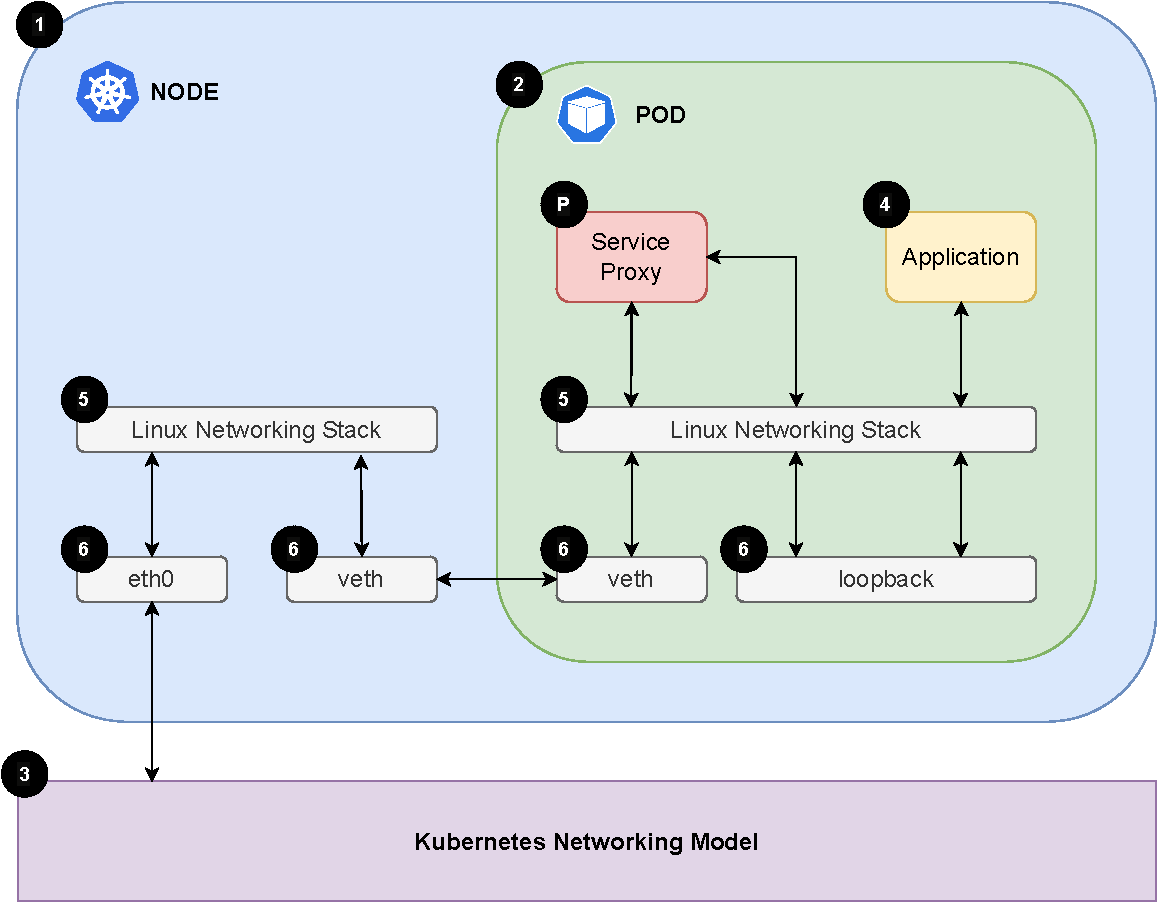
\includegraphics[width=\linewidth]{3_systems_survey/figures/sm-arch-per-service.pdf}
    }

    \caption[Per-service proxy plane architecture.]{The data path of a per-service data plane.}
    \label{fig:sm-arch-per-service}
\end{figure}

% Basic components introduction
First off, we have the node (\designref{1}), this represents a worker machine in \gls{k8s}, which can run workloads. Next up, we have a \gls{pod} (\designref{1}), this is the smallest unit of deployment within \gls{k8s} and consists of one or more application containers. The last \gls{k8s} related concept is the Kubernetes Networking Model (\designref{3}) \cite{kubernetes-cluster-networking}, which can be implemented in various ways, but has as goal to connect the nodes and pods within the cluster. Within the \gls{pod}, lives the actual application (\designref{4}), which can for example be a web server. The \textit{Linux Network Stack} (\designref{5}) is abstracted in this design as one single component, but consists of routing and filtering tables used to manage packets within the system. An important note, is that both the node and the \gls{pod} implement a separate networking stack, which isolates the pod network from the host network through network namespaces \cite{man-network-namespaces}. The traffic flows to physical and virtual network interfaces (\designref{6}) connected through one another, to reach its destination. Note that in actual deployments, more complex models are often present, such as bridge networks to support multiple pod networks or tunnel interfaces to create overlay networks, for instance. However, for this example, the added complexity does not help to illustrate the architectural differences at hand.


% Explain datapath
With the basic components of the reference architecture explained, we can take a closer look at the data path of a service request. Whenever a request to a service has been made that lives within the application pod (\designref{4}) a packet first enters the node. The inbound packet enters through the network interface (\designref{6}), has to pass through the kernel's networking stack (\designref{5}) to reach the \gls{pod}'s network namespace. After this, the traffic will reach the service proxy (\designref{P}) because it is configured to intercept all network traffic inside the pod. From there onwards, it has to travel through a loopback interface to finally reach the application. Replies from the application will traverse a similar, but inverse, data path.

% Advantages/Disadvantages
One of the advantages of such an architecture is that you can have fine-grained control over the traffic, as it is intercepted the moment it enters the namespace of the \gls{pod}. This characteristic allows the security features discussed during this systems review (\ref{fr-2}), and can for example enable encrypted connections between all traffic leaving a \gls{pod}. Furthermore, the \textit{sidecar pattern} allows for a very generic implementation, and does not require much if any modifications from the user's perspective. This enables a user-friendly user experience, while also allowing support for general purpose proxies such as \textit{Envoy} or \textit{HAProxy}. These advantages, make it so that this is the most common architectural approach identified. A disadvantage, however, is that this design introduces additional overhead. First off, it introduces an overhead in system resources, as there now is a network proxy for every software service. Furthermore, it introduces additional latency for the traffic, as for every service request, the packets travel through the proxy twice (ingress/egress).


\subsubsection{Per-Node Proxy}
\label{sec:survey:analysis:architectures:per-node}
% - Less overhead and hops
% - No MTLS

Another identified \gls{sm} architecture makes use of the per-node proxy. This architectural style is used by a single identified \gls{sm} system, \textit{Traefik Mesh}. We present this form of \gls{sm} architecture in \cref{fig:sm-arch-per-node}. Although many of the components in this system are similar and previously explained in \cref{sec:survey:analysis:architectures:per-service}, some differences change several characteristics drastically.

\begin{figure}[!t]
    \centering
    
    \scalebox{.8}{
    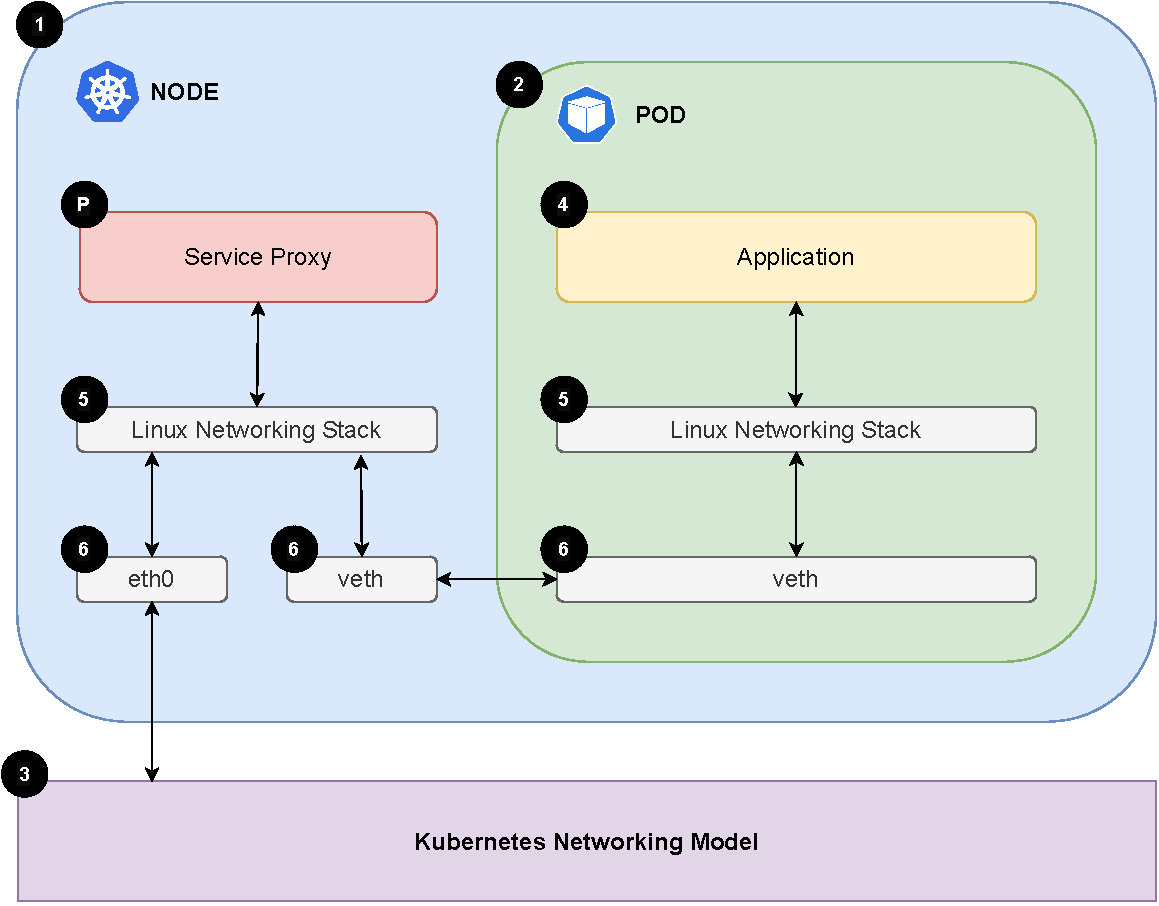
\includegraphics[width=\linewidth]{3_systems_survey/figures/sm-arch-per-node.pdf}
    }
    
    \caption[Per-node proxy plane architecture.]{The data path of a per-node data plane.}
    \label{fig:sm-arch-per-node}
\end{figure}

The most significant difference compared to the per-service architectural style is that service proxy (\designref{P}) is now not embedded within the \gls{pod} but lives within the node, thus makes use of the host network namespace. The reason for this is that this architectural style tries to limit the additional overheads caused by the introduces proxies of a \gls{sm}. This style of service proxies results in a single proxy per node, and thus does not scale linearly with the number of services on a node. This leads to the advantage that it consumes less system resources in the form of CPU cycles and memory. An additional benefit of this approach is that the traffic in the data path now has to traverse the proxy once in a service-to-service request. This halves the amount of service proxy hops compared to the previous solution. 

However, this architectural pattern comes at a cost. Since the traffic is not passing through the service proxies from within the pod, traffic enters the host network in a potentially compromised state. To elaborate this, the per-service approach allowed the traffic between proxies to be automatically encrypted using a mutual TLS connection, a characteristic evaluated during the system's review (\ref{fr-2}). This is, however, not possible as the data path outside the \glspl{pod} is not fully controlled and therefore has to be implemented manually. A downside is that when this is ignored, service-to-service data flows unencrypted through the node and therefore breaches well established security best practices such as the notion of zero trust networks \cite{zero-trust-network}.




\subsubsection{eBPF Proxy}
\label{sec:survey:analysis:architectures:ebpf}
% - New area
% - Faster, less hops
% - Potential security risks?
% -- Programmable Sandbox in kernel space

The last of the identified \gls{sm} architectures uses a vastly different approach. The approach used by \textit{Cilium} uses \gls{ebpf} to establish a mesh network between the services. What started out as a \gls{k8s} networking solution and evolved to become a fully fledged \gls{sm} implementation \cite{cilium-mesh}. 

% Shortened data path
In \cref{fig:sm-arch-ebpf}, we present a simplified data path of a \gls{sm} implemented using \textit{Cilium}.  Many of the components are shared with the other architectures and are explained in \cref{sec:survey:analysis:architectures:per-service}. However, compared to the other identified architectures, the data path as depicted here is much shorter. This is because the routing and proxying is done in the kernel through \gls{ebpf} (\designref{P}). 

% Explain EBPF
To explain the shortened data path, we first briefly have to introduce the technology powering it. \gls{ebpf} is a Linux Kernel technology that allows users to run sandboxed programs in the operating system kernel \cite{ebpf}. Furthermore, it is event-driven and allows these programs to execute on certain hooks. This is used throughout \textit{Cilium} to implement the observability, security and networking functionalities of the \gls{sm}. \gls{ebpf} allows for hooks throughout the entire lifecycle of a network packet. This combined with the programmable sandbox environments allows it to replace the role of service proxies in the other architectural styles. Since the \gls{ebpf} programs are aware of the \gls{k8s} endpoints and services, packets can be routed straight from the kernel, enabling a much more direct route.

% Advantages/Disadvantages
This architectural style has several advantages compared to the previously introduced per-service and per-node architectures. First, it has potential to decrease latency in its data path. It does this by not requiring additional hops in service-to-service communications. Additionally, it allows for greater programmability of the mesh network, as certain programs can be compiled and then run in a sandboxed environment. However, it also can have some disadvantages. First off, the technology and this implementation of it in particular is fairly new, even in a beta phase at the time of writing. This means that the \gls{sm} implementation could be unstable and not suitable for production usage. Furthermore, using user programs in kernel space could introduce potential security risks. 


\begin{figure}[!t]
    \centering
    
    \scalebox{.8}{
    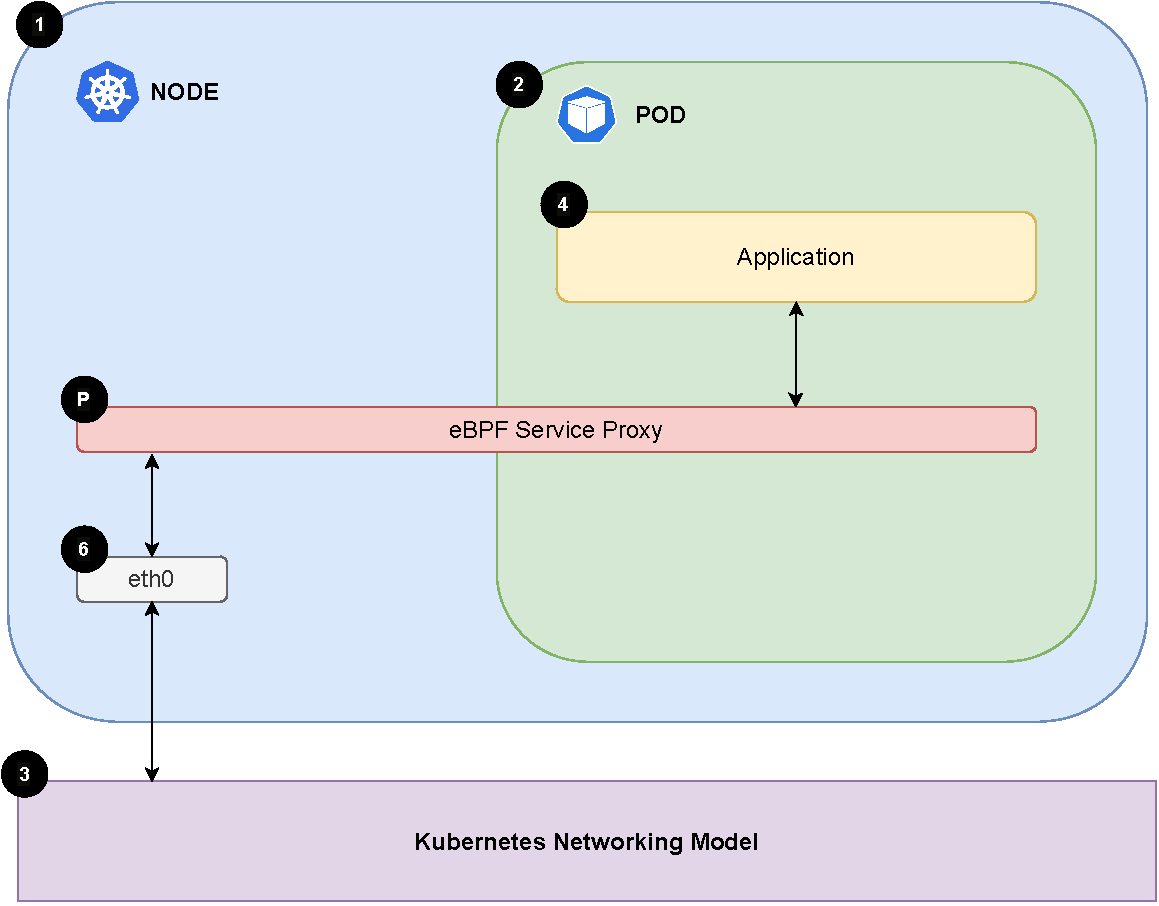
\includegraphics[width=\linewidth]{3_systems_survey/figures/sm-arch-ebpf.pdf}
    }
    
    \caption[\Gls{ebpf}-based data plane architecture.]{The data path of an \gls{ebpf}-based data plane.}
    \label{fig:sm-arch-ebpf}
\end{figure}


\subsection{Conclusion}
\label{sec:survey:analysis:conclusion}

To conclude the systems survey, we return to the initial research question (\ref{rq-1}), \textit{How do existing \gls{sm} implementations compare?}. The answer to this question is provided in various levels of detail throughout the systems survey. The most detailed and objective answer is provided  within the data synthesis and results section (\cref{sec:survey:results}) in which we identified domain-specific characteristics and features and compared the systems based on that. A summarized result is presented in the form of established functional and non-functional requirements (\cref{sec:survey:analysis}), in which we combine results from the data synthesis to provide a more generic, but more useful result. Finally, in \cref{sec:survey:analysis:architectures}, we take a deep-dive into the architectural differences of identified systems in which we answer the research question by exploring key characteristics in more detail.

Throughout this systems survey, we observed that \gls{sm} systems can have different approaches and goals and that systems within this the area are constantly changing. With many of the systems adopting different strategies and bleeding-edge technologies, the area is exciting in many ways. 
	
% Setup
\graphicspath{./figures}

\chapter{Design and Implementation of a Service Mesh Benchmark}
\label{chap:system-design}

% Introduction
% - What will this chapter contain and what resaarch question it tries to answer

% Prev chapter -> General
% This chapter -> Performance oriented + importance
In the previous chapter (\cref{chap:survey}), we conducted a systems survey and identified several state-of-the-art \gls{sm} systems. We examined the architectural differences between these systems and compared them on domain-specific functional and non-functional requirements. We then discussed the theoretical performance implications of the architectural styles that we had identified. These performance implications have an effect on the performance of all software services in an environment and can cause a major bottleneck. With these concerns in mind, we dive deeper into the performance of \gls{sm} systems.


% Which RQ will we answer
% Related work -> Shortcomings
% What we do to solve these shortcomings
In this chapter, we provide an answer to research question \ref{rq-2}. \textit{How to design and implement a \gls{sm} benchmark which evaluates the performance of \gls{sm} systems?} During the systems survey, we observed that there was no relevant work found in the \gls{pl}. Furthermore, preliminary research has shown that previous and current efforts made to evaluate these performance characteristics are either in early stages or have limited functionality. To solve these shortcomings, we present a \gls{sm} benchmark instrument and implement a prototype that supports various workloads, application level protocols and \gls{sm} systems.

% Rest of the chapter is structured as follows
% - The need for these surveys (related work)
% - Methodology used for both surveys
% - Results of 
The remainder of this chapter is structured as follows. First, in \cref{sec:system:objectives} we introduce the goals of the benchmarking instrument. Second, in \cref{sec:system:sut} we describe the components that are part of the \gls{sut}. Afterwards, in \cref{sec:system:requirements-analysis} we present a requirement analysis in which we formalize the stakeholders, use cases and system requirements of the instrument. Next, in \cref{sec:system:design} we present the design of the \textit{Mesh Bench}, a benchmarking instrument for \gls{sm} systems. Finally, in \cref{sec:system:implementation} we discuss the implementation details of a prototype system. 

% Finally, in \cref{sec:system:analysis} we analyse the proposed design and implementation.

\section{Benchmarking Objectives}
\label{sec:system:objectives}

% What are we trying to achieve with this benchmarking instrument
% - Analyize introduced latency
% - Analyze overhead in system resources CPU/mem
% - Analyze the maximum throughput of the system
% - Analyze protocol differences

The goal of a benchmarking instrument is to objectively compare, and decide on the best system for a particular domain. However, the concrete definition of the best system depends on the underlying benchmarking objective \cite{folkerts2012benchmarking}. Therefore, it is important to first establish a set of goals for the benchmarking before designing or implementing it. In this section, we will introduce the benchmarking objectives, related to the main research question \ref{rq-2}.

To design a benchmark that evaluates key characteristics of a \gls{sm} system, we guide the process by following industry best practices for measuring and monitoring distributed systems. Following the best practices and principles of the Google Site Reliability Engineering handbook \cite{beyer2016}, we can establish a base set of metrics and signals that are important to measure in distributed systems. More specifically, we can follow the guidelines for \textit{white-box monitoring} and implement the  \textit{Four Golden Signals} in our benchmarking instrument.

The following list presents the objectives that the benchmarking instrument has.

\begin{enumerate}[label=\textbf{O\arabic*}, leftmargin=3\parindent]
    \item \textbf{Support System Resource Measurements}
    \label{o-1}
    
    The first objective of the benchmarking instrument is to measure the amount of system resources a \gls{sm} system uses.
    
    \item \textbf{Support Throughput Measurements}
    \label{o-2}
    
    The second objective is to measure the amount of throughput a system can handle. The throughput in this context refer to the number of requests per pre-defined time frame a \gls{sm} system can handle. This is used to see if the \gls{sm} system introduces any bottleneck in terms of throughput.

    \item \textbf{Support Latency Measurements}
    \label{o-3}
    
    The third objective is to measure the amount of latency requests have. This is used to measure how much latency a \gls{sm} system introduces.

    \item \textbf{Support Resiliency Measurements}
    \label{o-4}
    The final objective of the instrument is to measure the resiliency of the systems by measuring the error rates within the system.
    
\end{enumerate}

\section{System Under Test}
\label{sec:system:sut}
% Explain SUT
% Components of Interest
% Purely Functional Components
% Present SUT

To design a benchmarking instrument that evaluates \gls{sm} systems, we first have to define the system and the components that are included in the benchmark. The components relevant to the benchmark are described in the \gls{sut}. However, even though the benchmark has to deal with numerous components in the system, not all are relevant to the benchmark.

Therefore, we split the components of the \gls{sut} in two categories according to the practices outlined by Folkerts et al. \cite{folkerts2012benchmarking}. The first group of components are labelled \textit{Components of Interest}. These components are of principal interest to the benchmark and have to be measured. The second group of components is labelled as \textit{Purely Functional Components}. The components in the latter group are present in the \gls{sut} in order for the benchmarking instrument to work correctly. However, measuring these components is not of importance relating to the objectives of the benchmark.

In \cref{fig:sut} we present the \gls{sut} for the benchmarking instrument. In the following sections, we elaborate on the  \textit{Components of Interest} (\cref{sec:system:sut:components-interest}) and \textit{Purely Functional Components} (\cref{sec:system:sut:components-functional})  present in this system.

\begin{figure}[!t]
    \centering
    
    \scalebox{.8}{    
    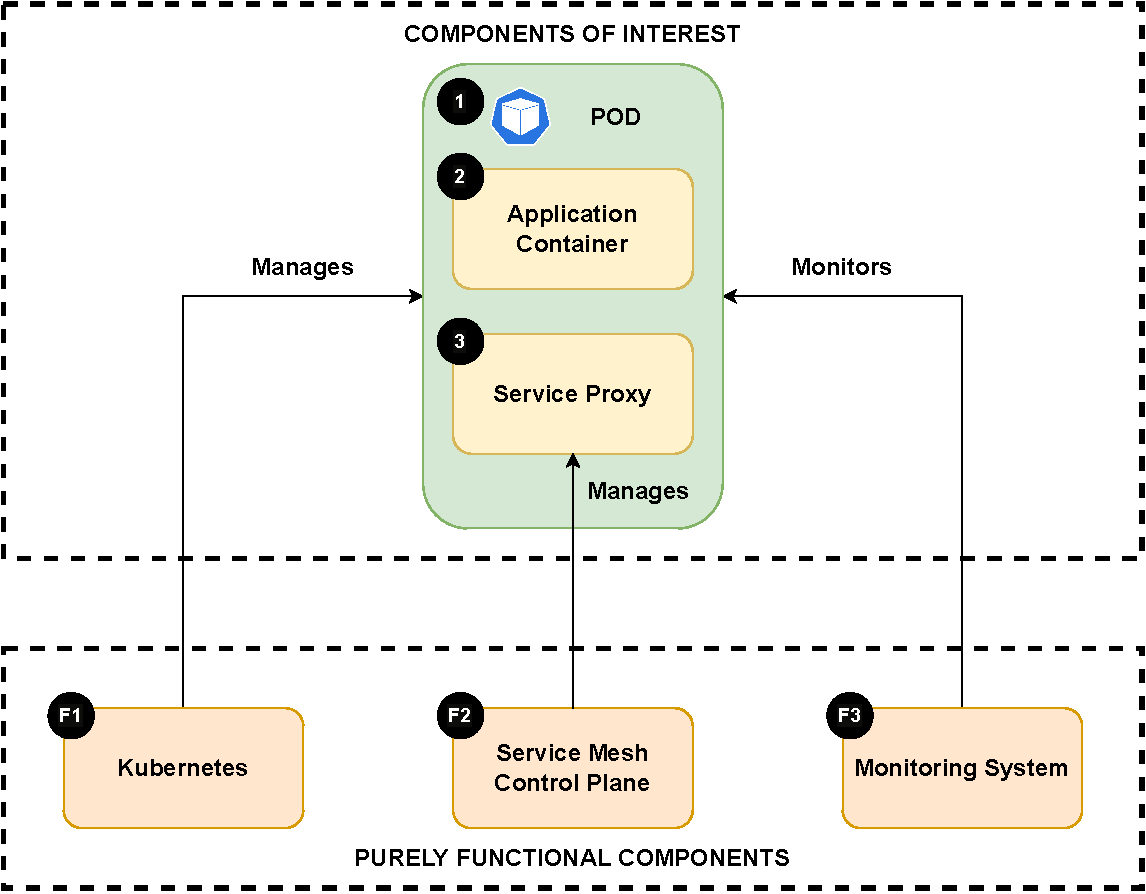
\includegraphics[width=\linewidth]{4_system_design/figures/system-under-test.pdf}
    }
    
    \caption{The \gls{sut} for benchmarking \gls{sm} systems.}
    
    \label{fig:sut}
\end{figure}
\todo{figure: move service proxy halfway between pod/nothingnes?}

\subsection{Components of Interest}
\label{sec:system:sut:components-interest}
% Elaborate on the components of interest
% Data Path of Traffic
% Pod containing the service
% - Application Pod
% - Service Mesh Proxy (data plane)

The \textit{Components of Interest} are aligned with the objectives as presented in \cref{sec:system:objectives}. In the context of a \gls{sm} system, we aim to measure the components present in the data path of a software service. Therefore, in the context of a \gls{k8s} cluster running a \gls{sm} we evaluate the performance of software services that live in the \gls{k8s} specific abstraction, the \gls{pod} \designref{1}.

To measure the service and the service traffic, we measure the application container \designref{2} and the data plane component of a \gls{sm} \designref{3}.

\subsection{Purely Functional Components}
\label{sec:system:sut:components-functional}
% Elaborate on the functional components
% Metric Services - Prom
% Control Plane components of sm
% - More detail?

To be able to run the benchmark, we require the several components. First, we run the benchmark on a \gls{k8s} cluster \designref{F1}. Furthermore, a \gls{sm} system introduces several control plane components, which are required for the service mesh to correctly function \designref{F2}. However, since our objectives are to measure the data path of a \gls{sm} they are not of importance to the benchmarking instrument. Additionally, we introduce a metrics and monitoring system in the cluster \designref{F3}, which will be used to collect and time series data of the pods and containers residing in the \gls{k8s} cluster.
\section{Requirements Analysis}
\label{sec:system:requirements-analysis}

In this section, we expand on the details and requirements of the benchmarking instrument. To properly define the requirements of the benchmark, we first have to define the stakeholders and their use cases for such an instrument. After that is defined, we can define the actual requirements of the instrument based on those.

In \cref{sec:system:requirements-analysis:stakeholders} we define the stakeholders. Afterwards, in \cref{sec:system:requirements-analysis:use-cases} we define the use cases for the benchmarking instrument. Finally, in \cref{sec:system:requirements-analysis:requirements} we define the actual requirements.


\subsection{Stakeholders}
\label{sec:system:requirements-analysis:stakeholders}
% Who are the stakeholders?
% End users (cluster operators)
% Developers of SM platforms
% Scientific users

To uncover the use cases of this benchmarking instrument, we first have to identify the primary stakeholders. This is because stakeholders can have different applications for such a system, and therefore have different requirements. The following list of stakeholders (\ref{sh-1}-\ref{sh-3}) introduces the identified stakeholders and their concerns.

\begin{enumerate}[label=\textbf{S\arabic*}, leftmargin=3\parindent]
    \item \textbf{DevOps Engineers}
    \label{sh-1}
    
    This group of stakeholders is the primary user of a \gls{sm} system. They manage and control the infrastructure applications and services run on, and therefore can consider implementing a \gls{sm} system. Their primary concern with the benchmarking instrument is to evaluate the performance and resiliency characteristics of a \gls{sm} implementation on existing infrastructure or compare different implementations to make an informed decision to choose between the various implementations. For this group of stakeholders, it is important that the \gls{sm} matches their goals and requirement. This is exemplified by a DevOps engineer bound to predetermined \glspl{sla} that define contracts on service latencies.
    
    \item \textbf{Service Mesh Engineers}
    \label{sh-2}
    
    The second group of stakeholders consists of the engineers that develop the \gls{sm} systems itself. For these engineers, it is important to track the performance of their system to make sure that it meets the predetermined performance requirements. Furthermore, it can enable the engineers to compare their system to other offerings in the \gls{sm} landscape, which can help this group to set expectations and requirements.
    
    \item \textbf{Scientific Researchers}
    \label{sh-3}
    
    The final group of stakeholders represents researchers from academic institutions. This group uses the benchmarking instrument to conduct scientific research on the \gls{sm} systems, and their workloads. For this group of stakeholders, it is important that the benchmark instrument reports detailed information on both the system and the workloads running on it so that they can reason on the results.  Furthermore, it is important that the results the instrument produces are reproducible, meaning that experiments conducted with similar inputs produce similar outputs (bearing in mind the inherent variability in distributed environments). Finally, it is important that the instrument can run different workloads so that they can evaluate different situations and environments.
\end{enumerate}


\subsection{Use cases}
\label{sec:system:requirements-analysis:use-cases}
% What can this system be used for?
% https://www.similarweb.com/corp/blog/research/business-benchmarking/benchmarking-types/ -> Business benchmark translated to software
%  Competitive benchmarking –> See how one system compares to another
% Strategic benchmarking -> To look at the best performing system (in a category) to learn from
% Performance benchmarking -> Set targets of a system and evaluate over time
%  Validate Perforamnce Optimizations

Previously, we have identified the stakeholders of a benchmarking instrument, (\ref{sh-1}-\ref{sh-3}) as it is important to know the users and their concerns. This helps us to understand \textit{who} the users of the benchmark are, and \textit{why} they would use such an instrument.

To understand \textit{how} such a benchmark is used, we need to identify the use cases. Drawn from the concerns of the stakeholders, we present a list of use cases that (\ref{u-1}-\ref{u-3}) this benchmarking instrument can fulfil.

\begin{enumerate}[label=\textbf{UC\arabic*}, leftmargin=3\parindent]
    \item \textbf{Competitive Benchmarking}, \textit{concerns:} \ref{sh-1}, \ref{sh-2}, \ref{sh-3}
    \label{u-1}
    % Basic performance evaluation on multiple systems
    % Compare systems -> Which system is the best
    % Applies to: All
    
    The first and most common use case of the benchmarking instrument is to perform competitive benchmarking. The benchmarking instrument produces quantitative data on the performance characteristics of a \gls{sm} system.  The results of the benchmark can then be used to compare \gls{sm} implementations and decide on the best performing system in a domain.
    
    \item \textbf{Strategic Benchmarking}, \textit{concerns:} \ref{sh-2}, \ref{sh-3}
    \label{u-2}
    % Look at best system in category x
    % Look at the implementation details of that system (regarding category x)
    % Learn from it -> Apply
    % Applies to: Engineers, Academia
    
    % \todo{Bench use case: mb rename strategic?}
    
    A second use case of the benchmarking instrument is to enable critical insights into the best performing systems. A benchmarking instrument gives insights into the performance of various characteristics of a system. This allows users to analyse the best performing systems in certain individual areas. Analysing those systems in further detail allows users to develop an understanding on how these systems achieved their results and allows them to learn from it. These critical insights can then be translated into other systems applying these best practices.
    
    \item \textbf{Evaluate Periodic Performance}, \textit{concerns:} \ref{sh-1}, \ref{sh-2}, \ref{sh-3}
    \label{u-3}
    % Compare the performance of a single system over time
    % Applies to: All
    
    A third use case for the benchmarking instrument is to capture the performance of a system over time. When conducting a benchmark, you evaluate a system and capture the performance of that system at a specific time. However, it can also be used to monitor and evaluate the performance of a system over a larger time frame to determine if, and by how much, the performance characteristics alter over time.
    
    
    \item \textbf{Validation of Performance Optimizations}, \textit{concerns:} \ref{sh-2}, \ref{sh-3}
    \label{u-4}
    % Developers -> Test changes to a sm system
    % See if perforamnce differs over versions
    % Applies to: Engineers, Academia

    Another use case for this benchmarking instrument is to analyse the impact of performance optimizations applied to \gls{sm} systems. When such an optimization is made, users can evaluate the system pre- and post-optimization to measure the impact of the optimization.
    

    \item \textbf{Validate System Requirements}, \textit{concerns:} \ref{sh-1}
    \label{u-5}
    % Evaluate if a sm implementation could be used in the environment oof the end user
    % e.g. SLA (min latency
    % Applies to: DevOps (end user)
    
    A final use case for this benchmarking instrument, is to evaluate if a \gls{sm} meets the requirements of the end user. End users can have different requirements, such as performance and resiliency requirements. This benchmark will enable those users to evaluate a \gls{sm} on their infrastructure to see if the system meets their requirements.
    
\end{enumerate}

\subsection{Requirements}
\label{sec:system:requirements-analysis:requirements}
% Introduce the requirements of the system
% Based on Folkters et al. three types of requirements
% - General Requirements
% - Implementation Requirements
% - Workload requirements

To design a benchmarking instrument that resembles any value, we satisfy the concerns and use cases of the identified stakeholders. To ensure that we satisfy this, we formulate a set of requirements, which we present in the following sections.

\subsubsection{Functional Requirements}
\label{sec:system:requirements-analysis:functional}

Functional requirements are requirements that the system \textit{must} implement, to function correctly. The following list (\ref{system:fr-1} - \ref{system:fr-7}) introduces the functional requirements of the benchmarking instrument and to which use case they relate.

\begin{enumerate}[label=\textbf{FR\arabic*}, leftmargin=3\parindent]
    \item \textbf{Support the most popular \gls{sm} implementations.}, \textit{related to:} \ref{u-1},  \ref{u-3}, \ref{u-4}
    \label{system:fr-1}
    
    The benchmarking instrument must support the most popular \gls{sm} implementations. During the systems survey (\cref{chap:survey}), we identified that two of the identified \gls{sm} implementations currently dominate the landscape in terms of usage \cite{cncf-survey-2021}. Therefore, the benchmarking instrument has to support both \textit{Istio} and \textit{Linkerd} to be relevant for most users. 
    
    \item \textbf{Support systems using different data plane architectures}, \textit{related to:} \ref{u-1}, \ref{u-3}
    \label{system:fr-2}
    
    The benchmarking instrument must support all the identified data plane architectures (\cref{sec:survey:analysis:architectures}). During the systems survey, we identified four different data plane architectures with various performance implications. To analyse this, the benchmark must support at least one of the identified systems for each identified data plane architecture. The system already has to support systems adhering to the \textit{per-service} through the first established functional requirement (\ref{system:fr-1}). Since the other architectures only relate to a single \gls{sm} implementation, it means that the system must additionally support  \textit{Cilium} and \textit{Traefik}.
    
    \item \textbf{Implement and Report the Four Golden Signals}, \textit{related to:} \ref{u-1}, \ref{u-2}, \ref{u-3}, \ref{u-4}, \ref{u-5} 
    \label{system:fr-3}
    
    The benchmarking instrument must implement the \textit{Four Golden Signals}. To report meaningful data, we have to define meaningful metrics that the benchmarking instrument will report. To achieve this, we define the metrics by following industry best practices as established in the Google SRE handbook \cite{beyer2016} and implement the \textit{Four Golden Signals}. This means that the benchmarking instrument must implement relevant metrics to report the \textit{Latency}, \textit{Traffic}, \textit{Errors}, and, \textit{Saturation} of the \gls{sut}.
    
    \item \textbf{Support Varying Workloads}, \textit{related to:} \ref{u-2}, \ref{u-3}, \ref{u-5} 
    \label{system:fr-4}
    
    The benchmarking instrument must support varying workloads. This allows the benchmark to be relevant for the different use cases it can encounter and simulate the different workloads a \gls{sm} can see in the real world. To support this, the benchmark must provide a mechanism to specify the workload that the benchmark will run. Additionally, it has to provide a way in which the user can specify how the benchmark can extract relevant metrics. This is done by specifying how the workload, or service, can be consumed (e.g. HTTP endpoints).
    
    \item \textbf{Support Varying Cluster Environments}, \textit{related to:} \ref{u-2}, \ref{u-3}, \ref{u-5} 
    \label{system:fr-5}
    
    The benchmarking instrument must support varying cluster environments. This means that the benchmark must support any valid \gls{k8s} cluster environment. This allows users to evaluate \gls{sm} implementations on within their own environment and enables environment-specific use cases such as \ref{u-5}.
    
    \item \textbf{Report results in a well-known data format}, \textit{related to:} \ref{u-1}, \ref{u-2}, \ref{u-3}, \ref{u-4}
    \label{system:fr-6}
    
    The benchmarking instrument must report its results in a well-known data format. In order for the results to be useful to the various stakeholders, data must be presented in well-known formats such as \textit{JSON}, \textit{CSV} or \textit{YAML}.
    
    
    \item \textbf{Produce Reproducible Results}, \textit{related to:} \ref{u-1}, \ref{u-2}, \ref{u-3}, \ref{u-4}, \ref{u-5} 
    \label{system:fr-7}
    
    The benchmarking instrument must produce reproducible results. To provide meaningful results, the instrument has to be able to produce similar results when running a single experiment in the same environment. If the instrument is given the same inputs, similar outputs have to be expected.
    
\end{enumerate}


\section{Design of a Service Mesh Benchmarking Instrument}
\label{sec:system:design}

In this section, we present the design for \textit{Mesh Bench}, a benchmarking instrument for \gls{sm} systems. In \cref{fig:benchmark-design} we depict an overview of the benchmark and all of its components. This design shows how a user interacts with the benchmark, and how it can evaluate the components within the \gls{sut} (see \cref{sec:system:sut}). In the remainder of this section we will introduce the annotated components (as indicated by the black circles \designref{1} - \designref{8}) and discuss the functionalities of them.

\begin{figure}[!t]
    \centering
     
    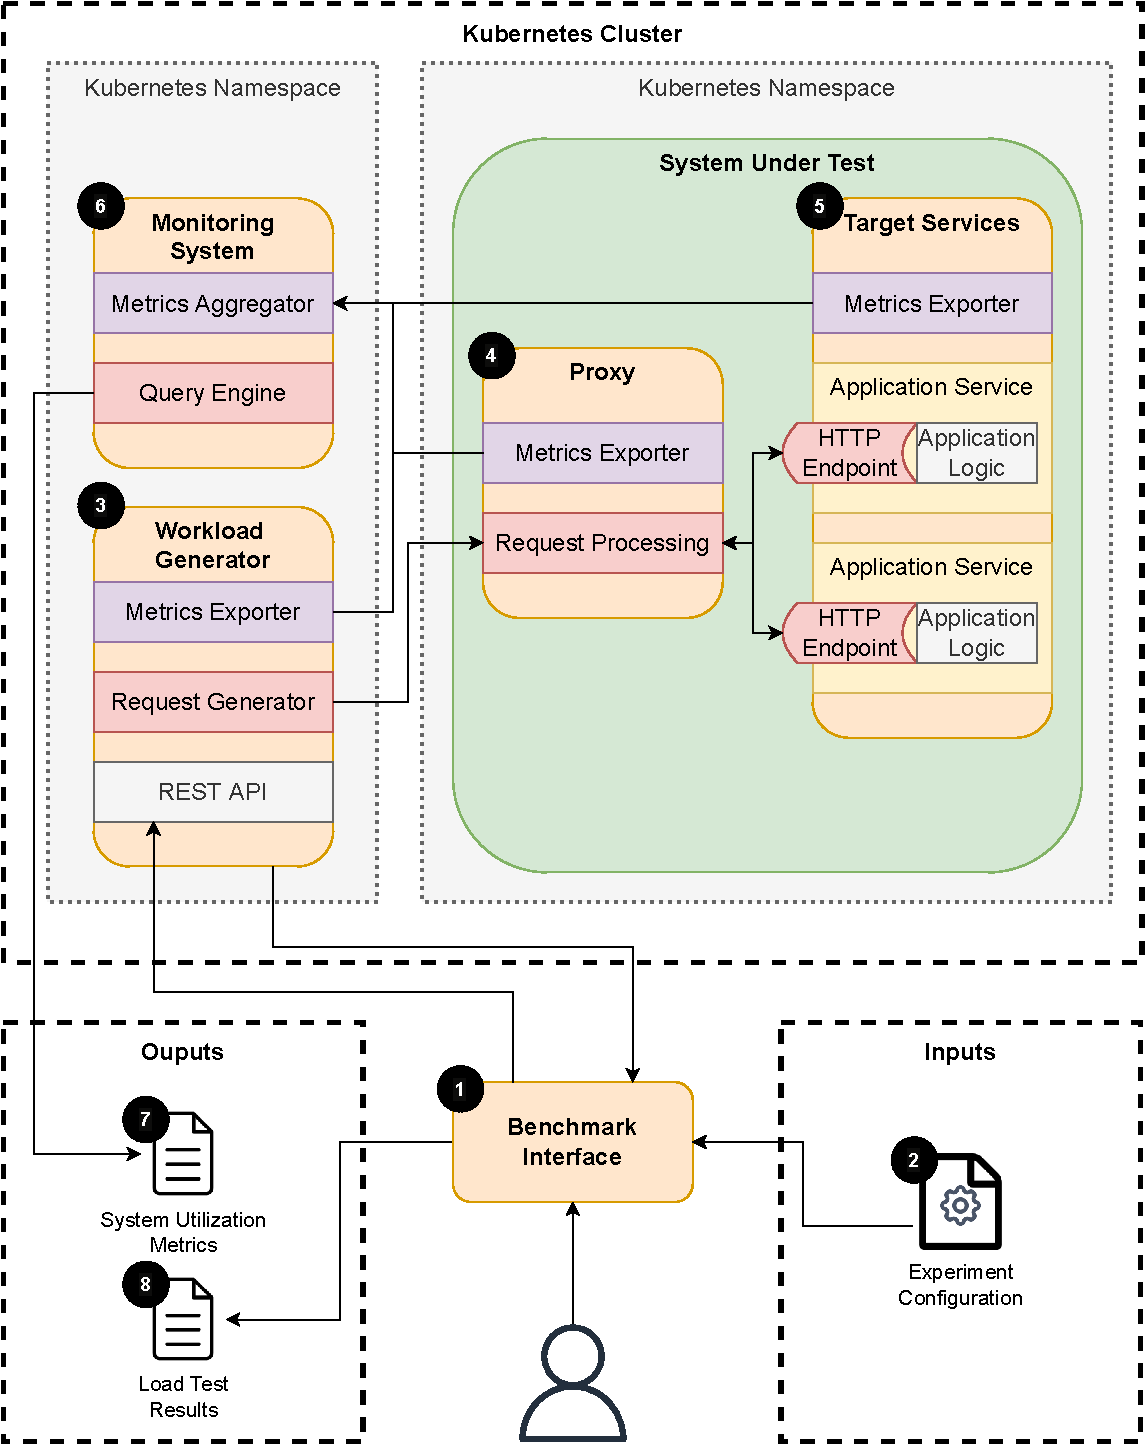
\includegraphics[width=0.9\linewidth]{4_system_design/figures/detailed-benchmark-design.pdf}
    
    \caption[Design of \textit{Mesh Bench}.]{A design overview of \textit{Mesh Bench}, a benchmark for \gls{sm} systems.}
    
    \label{fig:benchmark-design}
\end{figure}



\subsection{Benchmark Interface}
The \textit{Benchmark Interface} \designref{1} is the entry point for the end user and enables them to conduct performance experiments on \gls{sm} systems. The main goal of the Benchmark Interface is to manage experiment executions. The lifecycle of a single experiment consists of three phases. The first phase consists of initialization and configuration. This is done by parsing and processing an \textit{Experiment Configuration} \designref{2}. After this, it instructs the \textit{Workload Generator} \designref{3}, to generate experiment-specific workloads based on the supplied configuration. Once an experiment is finished and the workload generator has reported back to the benchmark interface, it finalizes the experiment and stores the obtained results \designref{8}.

\subsection{Experiment Configuration}
The benchmark consists of several performance experiments, as introduced in \cref{chap:experimental-evaluation}. Each of these experiments consists of several configuration parameters, which allows the user to change several aspects of the experiment. Notable configurations include the ability to modify the type of workload, the frequency of the workload, the duration of the experiment and what type of workload to use, and therefore which target service \designref{5}. These configuration parameters of a single experiment, forms the \textit{Experiment Configuration} \designref{2} and is the primary input of the benchmark interface \designref{1}.


\subsection{Workload Generator}
The \textit{Workload Generator} \designref{3} is used to generate synthetic workloads and measure the performance of the components within the \gls{sut}. This is arguably the most important component in the benchmark, and it has to support various modes of operation to match the functional requirements as defined in \cref{sec:system:requirements-analysis:functional}. The workload generator has to be able to perform load test experiments, in which the \textit{Request Generator} generates a certain application workload for a given \textit{Target Service} \designref{5}. It has to be able to do so in a constant throughput fashion, i.e., a fixed number of requests per second while also supporting a mode that enables us to test the maximum throughput of a given \gls{sut}. Another important aspect is that it should be configurable at run-time, so that the benchmark interface \designref{2} can configure it, allowing us to design various performance related experiments. This aspect is done through the \textit{REST API} as depicted in the benchmark design. The workload generator also exposes system utilization metrics through the \textbf{Metrics Exporter}.

\subsection{Proxy}
The \textit{Proxy} \designref{4} is the core component of a \gls{sm} architecture. The entire benchmark is designed to measure the performance implications of the proxy component. This component varies based on the \gls{sm} system that is evaluated (see \cref{sec:survey:analysis:sm-framework} for the proxies used per \gls{sm} system). Furthermore, it is unmodified, which means that it will intercept all the requests from and to the target service \designref{5}, and do the \textit{Request Processing} as originally intended. However, we do export the resource utilization metrics through the \textit{Metrics Exporter}.

\subsection{Target Services}
At the receiving end of the requests as generated by the workload generator are the \textit{Target Services} \designref{5}. The goal of this component is to mimic a generic service as encountered in a production environment. In this benchmark, we have two \textit{Application Services} to mimic different types of workloads. The first type of service accepts workloads through the \textit{HTTP endpoint}. The second type of service accepts workloads through its \textit{GRPC endpoint}. Both of the backing services accept the synthetic workloads, and perform minimal to no computations on it (\textit{Application Logic)}. This minimizes the impact on end-to-end latencies observed and keeps the resource overheads to a minimum. This allows us to focus on the performance implications of the proxy, instead of the backing services. Just like the other components in the benchmarking system, we export resource utilization metrics through the \textit{Metrics Exporter}.


\subsection{Monitoring System}
The \textit{Monitoring System} \designref{6} is responsible for monitoring the systems within the \textit{Kubernetes Cluster}. This is used primarily to collect resource utilization metrics for all the components within the system through the \textit{Metrics Aggregator}. The monitoring system has to support the collection of these metrics at a fine granularity. More specifically, it has to be able to distinguish resource utilization metrics at a pod and container granularity. This allows us to identify resource utilization patterns for the components of interest. A user should be able to query the aggregated metrics through a \textit{Query Engine} and output these results in a common format to stable storage in a common format \designref{7}.


\subsection{Load Test Results}
The \textit{Load Test Results} \designref{8} are the results created by the \textit{Workload Generator} \designref{3}. These results contain the performance results of an experiment. More specifically, it contains the request latencies as generated by the workload generator. Additionally, it comes with metadata such as the experimental configuration and environment data. 

\section{Implementation}
\label{sec:system:implementation}

\subsection{Workload Generator}
\label{sec:system:workload-generator}

Fortio load generator (REST MODE)

\subsection{Target Service}
\label{sec:system:target-service}

Fortio HTTP echo service
Fortio gRPC healthz service

\subsection{Monitoring System}
\label{sec:system:monitoring-system}

Prometheus + Grafana
% \section{Analysis}
\label{sec:system:analysis}

A benchmarking instrument is successful if all the stakeholders agree it provides meaningful results. To analyse if the proposed implementation satisfies this we use a set of guidelines established by Folkerts et al. \cite{folkerts2012benchmarking}. In their work they establish three groups of requirements which can be used to evaluate ea benchmarking instrument.

In the remainder of this section we introduce these three groups of requirements and evaluate them against the proposed benchmarking instrument. 

\subsection{General Requirements}
\label{sec:system:analysis:general}
% General Requirements – this group contains generic requirements.

The \textit{General Requirements} group establishes four broad requirements (\ref{gr-1} - \ref{gr-4}). The following list introduces those requirements and discusses how the proposed benchmarking instrument satisfies the conditions.

\begin{enumerate}[label=\textbf{GR\arabic*}, leftmargin=3\parindent]
    \item \textbf{Strong Target Audience}
    \label{gr-1}
    % The target audience must be
    % - considerable size and,
    % - interested to obtain the information.
    

    \item \textbf{Relevant}
    \label{gr-2}
    % The benchmark results have to measure the performance of the typical operation within the problem domain.
    

    \item \textbf{Economical}
    \label{gr-3}
    % The cost of running the benchmark should be affordable.
    

    \item \textbf{Simple}
    \label{gr-4}
    % The benchmark should be understandable, as it creates trust.
    
\end{enumerate}


\subsection{Implementation Requirements}
\label{sec:system:analysis:implementation}
% 2. Implementation Requirements – this group contains requirements regarding

The second group of requirements introduced in the work of Folkerts et al. is the \textit{Implementation Requirements} and establishes requirements (\ref{gr-1} - \ref{gr-4}). The following list introduces those requirements and discusses how the proposed benchmarking instrument satisfies the conditions.


\begin{enumerate}[label=\textbf{IR\arabic*}, leftmargin=3\parindent]
    \item \textbf{Fair and Portable}
    \label{ir-1}
    % All compared systems can participate equally.

    
    \item \textbf{Repeatable}
    \label{ir-2}
    % The benchmark results can be reproduced by rerunning the
    
    \item \textbf{Realistic and Comprehensive}
    \label{ir-3}
    % The workload exercises all SUT features typically used in the major classes of target application

    \item \textbf{Configurable}
    \label{ir-4}
    % a benchmark should provide a flexible performance analysis framework allowing users to configure and customize the workload.
\end{enumerate}


\subsection{Workload Requirements}
\label{sec:system:analysis:workload}
% 3. Workload Requirements – contains requirements regarding the workload definition and its interactions.
The final group of requirements introduced is the \textit{Workload Requirements} and consists of three requirements (\ref{wr-1} - \ref{wr-3}). The following list introduces those requirements and discusses how the proposed benchmarking instrument satisfies the conditions.

\begin{enumerate}[label=\textbf{WR\arabic*}, leftmargin=3\parindent]
    \item \textbf{Representativeness}
    \label{wr-1}
    % The benchmark should be based on a workload scenario that contains a representative set of interactions.
    
    \item \textbf{Scalable}
    \label{wr-2}
    % Scalability should be supported in a manner that preserves
    
    \item \textbf{Metric}
    \label{wr-3}
    % A meaningful and understandable metric is required to report about the SUT reactions to the load

\end{enumerate}
	

% Setup
\graphicspath{./figures}

\chapter{Experimental Evaluation of Service Mesh systems}
\label{chap:experimental-evaluation}

% Introduction
% - What will this chapter contain and what resaarch question it tries to answer

% Prev chapter -> Design of the benchmark and implementation
% This chapter -> Design of experiments, conducting of experiments and results
In the previous chapter (\cref{chap:system-design}), we defined the \gls{sut} and the metrics that are important to evaluate the performance aspects of \gls{sm} systems. With this in mind, we designed and implemented a tool to benchmark the \gls{sut}. In this chapter, we present the experimental evaluation of \gls{sm} systems using the aforementioned benchmark. With this, we provide an answer to research question \ref{rq-3}. \textit{What are the differences between the different \gls{sm} systems in terms of overhead, throughput and latency?} 


% Rest of the chapter is structured as follows
% - Experimental Setup
% - Experimental Results
% - Analysis/Discussion
The remainder of this chapter is structured as follows. First, in \cref{sec:experiments:design} we introduce the design of the experimental setup. After that, in \cref{sec:experiments:results} we present and explain how to interpret the obtained results. Finally, in \cref{sec:experiments:discussion} we discuss the results and their implications.

\section{Experiment Design}
\label{sec:experiments:design}

% The goal of the experimental evaluation


The goal of the experimental evaluation is to gain insights into the performance characteristics of \gls{sm} systems. We do this by designing and conducting experiments to extract and gauge relevant metrics for these systems. This section builds upon the knowledge gained in previous chapters and details all the relevant aspects of the experiments.



\subsection{Service Mesh Selection}
\label{sec:experiments:design:meshes}
% What mesh setups did we choose?
% Why did we choose the service meshes included in the experiments?
% None -> Gives baseline
% Linkerd - Most popular (survey results)
% Istio - Most popular (survey results)
% Traefik - Per node arch
% Cilium - ebpf arch

The selection of \gls{sm} systems to include in the experiments is based on two criteria. First, we aimed to include a representative selection of systems that are used in real-world, production grade environments. Secondly, we aim to include systems based on different architectural approaches. In \cref{chap:survey}, we survey the existing state-of-the-art \gls{sm} systems in the industry and have identified the most frequently used, production grade systems. Furthermore, we identified three different architectural styles that could have major implications on the performance of these systems.

With this in mind we present the list of mesh configurations that is used throughout the experiments.

\begin{enumerate}[label=\textbf{SM\arabic*}, leftmargin=3\parindent]
    \item \textbf{None (baseline)}
    \label{exp:sm:0}
    
    To establish a baseline of performance, we start by performing experiments without any \gls{sm} at all. This enables us to not only compare different mesh systems to one another, but also allows us to paint a picture of the performance overhead compared to an unmeshed environment.
    
    \item \textbf{Istio}
    \label{exp:sm:1}
   
    The first mesh of the selection is \textit{istio}, we chose to include this \gls{sm} because of its prevalence in the industry. During our system survey we have identified that \textit{istio} is the most frequently used, production grade system at the time of writing.
    
    \item \textbf{Linkerd}
    \label{exp:sm:2}
   
    The second mesh of the selection is \textit{linkerd}, we chose to include this \gls{sm} because of its popularity. With a service proxy built for \gls{sm} workloads and a focus on performance, this system quickly gained popularity and established itself as a dominant entry in the industry.

    \item \textbf{Traefik}
    \label{exp:sm:3}
    
    The third mesh included in the experiments is \textit{traefik mesh}. We chose to include this mesh because it uses a vastly different architecture for its data plane. During our system survey we established that most of the identified \gls{sm} systems used a per-service proxy. \textit{traefik mesh} was the only system that we identified that used a \textit{per-node} proxy. By including this mesh in our experiments we aim to uncover the performance implications of this type of configuration.
    
    \item \textbf{Cilium}
    \label{exp:sm:4}
    
    The final mesh included in the experiments is \textit{cilium}. A rather new entry in the world of \gls{sm} systems that we chose to include because of its architecture. During our system survey we identified that \textit{cilium} was the only \gls{sm} system which used a \gls{ebpf} based data plane proxy. By including this mesh in our experiments we aim to expose the performance implications such architecture can introduce.

\end{enumerate}

\todo{add mesh versions, this table looks rather small}

Additionally, in \cref{tab:experiment:design:mesh} we present the versions used for each \gls{sm} during our experiments.

\begin{table*}[t]
\centering

\begin{tabularx}{\linewidth}{llX}

    \toprule
    Service Mesh       & Version & Reason for inclusion \\
    \toprule
    
    Cilium &
    v1.12.0-rc1 &
    The singular identified \gls{sm} system that uses an in-kernel, \textit{eBPF}-based data plane architecture.
    \\
    
    Istio &
    1.14 &
    Prevalence and market share.
    \\
    
    Linkerd2 &
    2.11.2 &
    Prevalence and market share.
    \\
    
    Traefik Mesh&
    1.4.5 &
    The singular identified \gls{sm} system that uses a per-node service proxy in its  data plane architecture.
    \\
    
    \bottomrule
    
\end{tabularx}

\caption[The \gls{sm} systems used in the experiments.]{The \gls{sm} systems used in the experiments and the reason of inclusion.}
\label{tab:experiment:design:mesh}
\end{table*}




\subsection{Metrics}
\label{sec:experiments:design:metrics}
% - System Resources
% - Throughput
% - Latency

To evaluate the performance characteristics of \gls{sm} systems we have to extract relevant metrics from the \gls{sut}. In \cref{chap:system-design}, we designed and implemented a benchmarking instrument to evaluate \gls{sm} systems. During the requirements analysis (\cref{sec:system:requirements-analysis}) we identified the stakeholders, discussed their use cases and formed a list of requirements. During this, we established a set of metrics that are used to evaluate the performance characteristics based on industry best practices.

Below we present the list of metrics used throughout the experiments

\begin{enumerate}[label=\textbf{M\arabic*}, leftmargin=3\parindent]
    \item \textbf{CPU utilization}
    \label{exp:metric:1}
    
    The first metric that we use during the experiments is related to resource utilization. This helps us to establish how much computational overhead the service proxies of a \gls{sm} introduce. All the CPU utilization results are expressed in fractions of a CPU core per second, e.g. the test system has 2 CPU cores and maximum utilization at a given time would be $2.0$. More specifically, we use the \Verb+container_cpu_usage_seconds_total+ as exposed through the \textit{Kubelet} process and obtain the results through \textit{Prometheus} using the query as seen in Listing \ref{lst:promql-cpu}.
    
    \begin{lstlisting}[caption=PromQL query for CPU metric, label=lst:promql-cpu] 
    sum(rate(
        container_cpu_usage_seconds_total{
            container!="",
            pod=~"(target-fortio|traefik-mesh-proxy|cilium).*"
        }[2s]
    )) by (pod, container)
    \end{lstlisting}

    
    \item \textbf{Memory utilization}
    \label{exp:metric:2}
    
    The second metric that we use in the experiments is also related to the resource utilization. We capture the memory utilization of service proxies by measuring the amount of memory they consume during operation. More specifically, we use the \Verb+container_memory_working_set_bytes+ as exposed through the \textit{Kubelet} process and obtain the results through \textit{Prometheus} using the query as seen in Listing \ref{lst:promql-memory}.
    
    
    \begin{lstlisting}[caption=PromQL query for CPU metric, label=lst:promql-memory] 
    sum(rate(
        container_memory_working_set_bytes{
            container!="",
            pod=~"(target-fortio|traefik-mesh-proxy|cilium).*"
        }[2s]
    )) by (pod, container)
    \end{lstlisting}

    
    \item \textbf{Requests per Second}
    \label{exp:metric:3}
    
    The third metric that we use is the amount of requests the system has handled expressed in requests per second. This metrics allows us to identify to measure the amount of throughput or traffic that a system can handle. 

    \item \textbf{Request Latency}
    \label{exp:metric:4}
    
    The fourth metric that we use in our experiments captures the amount of time it takes for a request to be served. This metric, is expressed as latency in milliseconds allows us to establish the overhead caused in the data path of every request in the system.

\end{enumerate}

In the experiments we do not evaluate metrics related to the resiliency of the system. In our requirements analysis we established a requirement to capture this characteristic based on established best practices. However, is not included in the current experimental design. The reason for this is twofold. First of, we uncovered that the \gls{sm} systems handle timeouts and errors in requests differently \cite{linkerd-retry} and that it involves balancing resiliency capabilities and system load. This means that we cannot compare the systems based on their default settings. Second, to create a fair experiment we have to configure these systems to have identical fault tolerance behaviours, which not all systems support. 


\subsection{Workloads}
\label{sec:experiments:design:workloads}
% GRPC Health
% HTTP echo

The selection of workloads aims to represent varying real-world scenarios that a \gls{sm} might encounter. Since a \gls{sm} handles most, if not all the traffic between software services, it can encounter a wide variety of workloads depending on the use case. With this in mind, we design our experiment to use workloads which are as generic as possible. 

During the systems survey conducted in \cref{chap:survey} we analysed the state-of-the-art \gls{sm} systems and identified their key \glspl{fr} and \glspl{nfr}. We identified that \gls{sm} systems handle service traffic in an application aware manner. Furthermore, we identified the most common application level transport protocols in terms of support. With this in mind, we designed the experiments around the two most common application level protocols. 

\subsubsection{HTTP Workload}
\label{sec:experiments:design:workloads:http}

For the experiments that make use of HTTP workloads we use a simple HTTP service. This service represents a simple echo service and replies with the data a client sends to it. This service requires relatively little system resources to operate and scales well to handle large amounts of connections. Additionally, it is also very configurable which enables us to test HTTP workloads with varying conditions and response payloads.

Although this is a synthetic workload which cannot be compared to any real-world workload, it allows us to capture and evaluate the general performance characteristics of \gls{sm} systems under varying circumstances.

\subsubsection{gRPC Workload}
\label{sec:experiments:design:workloads:grpc}

To evaluate how a \gls{sm} performs under varying application level workloads we included a GRPC workload. During the system survey we observed that all the identified \gls{sm} systems supported the \gls{grpc} protocol and noted that it was a common communication standard in distributed computing. With this in mind we introduced a simple \gls{grpc} based workload. To use the \gls{grpc} protocol, both the client and server need to know the service definition\footnote{\url{https://grpc.io/docs/what-is-grpc/core-concepts/\#service-definition}} since this varies from service to service. Best practices dictate that \gls{grpc} based services should to include a health checking endpoint\footnote{\url{https://github.com/grpc/grpc/blob/master/doc/health-checking.md}}. We use this to our advantage by using a simple \gls{grpc} service that includes this endpoint.

This synthetic workload is used to evaluate the performance implications of other (non-HTTP) application level workloads on \gls{sm} systems.

\subsection{Experimental Environment}
\label{sec:experiments:design:environment}
% Create repeatable experiments
% Cluster/Compute Setup
% Metric Collectors

It is important for experiments to be repeatable and that the variance is a little as possible. This allows others to reproduce and verify the results obtained and therefore be of scientific relevance. 

\subsubsection{Cluster Setup}
\label{sec:experiments:design:environment:cluster}

All the experiments were conducted on a \gls{k8s} cluster running on \gls{gcp}. The cluster was created through their managed \gls{k8s} service \gls{gke}. The decision to use their managed service to construct the cluster was based on their flexible, but vast array of network configuration options. In \cref{tab:experiment:design:cluster-config} we present the most important details of the cluster and node configurations used. Which we will now discuss in further detail.

First, we conducted all the experiments in the \textit{europe-west4} region. More specifically, all the compute nodes are located in the \textit{europe-west4-a} data centre location which is located at Eemshaven in the Netherlands. We chose this location as it was closest to our own location. Secondly, we used the most recent version of \gls{k8s} available at the time of writing in the stable release channel. Thirdly, we made use of \textit{VPC-native-routing}\footnote{\url{https://cloud.google.com/kubernetes-engine/docs/concepts/alias-ips}} which implements the \gls{k8s} networking model\footnote{\url{https://kubernetes.io/docs/concepts/services-networking/\#the-kubernetes-network-model}}. Additionally, we disabled \textit{Dataplane V2} an upcoming networking solution based on \textit{cilium} that would conflict with the \gls{sm} systems that we evaluate.

For the node configurations in the cluster we used a single \textit{e2-standard-2} node. This machine has 2 \textit{vCPUs} and 8 GB of memory\footnote{\url{https://cloud.google.com/compute/docs/cpu-platforms}}. We designed the experiments to be run on a single node cluster to abolish any variance in network latencies during the experiments. If for example, we chose to run the load generator on a single node and the target service on another node we introduce additional variance of network latencies.

\begin{table*}[!t]
\centering

\begin{tabular}{l r}


\toprule
\multicolumn{2}{c}{\textbf{GKE Configuration}}       \\
\toprule

\textbf{Compute Region}    & europe-west4            \\
\textbf{Kubernetes Version}& 1.22.8-gke.201          \\
\textbf{Kubernetes Release Channel} & regular        \\
\textbf{VPC-native-routing}         & enabled        \\
\textbf{Dataplane V2}               & disabled       \\

\toprule
\multicolumn{2}{c}{\textbf{Node Configuration}} \\
\toprule

\textbf{Compute Zone}               & europe-west4-a \\
\textbf{Node Count}                 & 1              \\
\textbf{vCPU}                       & 2              \\
\textbf{Memory}                     & 8 GB           \\  

\bottomrule

\end{tabular}


\caption{The cluster configuration used throughout the experiments.}
\label{tab:experiment:design:cluster-config}
\end{table*}

\subsubsection{Metric Collection}
\label{sec:experiments:design:environment:cluster}

We capture two types of metrics from the experiments. The first type of metric is related to the load generator (\ref{exp:metric:3}-\ref{exp:metric:4}). These metrics are collected by capturing the \gls{json} output that the load generator produces. The second type of metric is related to resource utilization (\ref{exp:metric:1}-\ref{exp:metric:2}). To analyse the resource overheads of data plane proxies we have to capture the resource overheads at a fine level of granularity, more specifically, at the level of a \gls{pod}.

To collect resource utilization at this level of granularity we bootstrap the cluster with various monitoring instruments. More specifically, we installed \textit{kube-prom-stack}\footnote{\url{https://github.com/prometheus-community/helm-charts/tree/main/charts/kube-prometheus-stack}}, an end-to-end monitoring solution based on the open-source monitoring solution \textit{Prometheus}\footnote{\url{https://prometheus.io/}}.


\subsection{Experiment Variables}
\label{sec:experiments:design:variables}

When performing load testing experiments we can observe and control many of the variables present in the environment. We can do so on three areas of the benchmark. First of, we can control which \gls{sm} is used, this will be done across all experiment. \cref{sec:experiments:design:meshes} details which \gls{sm} configurations are used and why they were chosen. Additionally, we can control the settings of the load generator. This allows us to tweak what kind of loads we can send (\cref{sec:experiments:design:workloads}) but also control how frequent we send loads and how to handle and or wait for responses. The final area which we can tweak is on the side of the target services. The target services are defined as the receiving endpoints of the load generator. This allows us to adjust the way a service responds, allowing us to introduce artificial delays, introduce faults or change payload sizes.

\begin{table*}[!t]
\centering

\begin{tabularx}{\textwidth}{l X r}

% Header
\toprule
\textbf{Variable}    &
\textbf{Description} &
\textbf{Default}     \\
\toprule

% Values
\textbf{Mesh Configuration} &
What type of \gls{sm} configuration is used in the experiment. (\cref{sec:experiments:design:meshes}) &
- \\

\textbf{Workload Type} &
What type of workload the load generator should send (\cref{sec:experiments:design:workloads}). &
HTTP \\

\textbf{RPS} &
How many requests per second the load generator should generate. &
100 \\

\textbf{Connections} &
Number of simultaneous connections to use when making requests. &
32 \\

\textbf{Duration} &
How long the load generator should generate load to the target service before aggregating and outputting results. &
15 minutes \\

\textbf{Payload Size} &
The size of the response payload in bytes. &
0 \\

\bottomrule

\end{tabularx}

\caption[Overview of the experiment variables.]{Overview of the experiment variables.}
\label{tab:experiment:design:exp-variables}
\end{table*}


In \cref{tab:experiment:design:exp-variables} we present the variables that we control across the experiments in this thesis. Additionally, it includes the default values that were used for these variables if they are not introduced as factor variables within an experiment.

\subsection{Experiments}
\label{sec:experiments:design:overview}

We now introduce the four experiments that were designed and used to evaluate the performance characteristics of \gls{sm} systems. For each of the experiments we introduce their primary goal, discuss how they are executed and reason why we chose this particular design. Additionally, \cref{tab:experiment:design:overview} presents an overview of all the experiments, what type of workloads they use, which  metrics they capture and which factors  are used to control the experiment.

\begin{table*}[!t]
\centering

\begin{tabularx}{\textwidth}{l l l X}

% Header
\toprule
\multicolumn{4}{c}{\textbf{Experiment Overview}} \\
\toprule

% Second Header
\textbf{Experiment}     &
\textbf{Workload}       &
\textbf{Metrics}        &
\textbf{Factors}        \\
\midrule

% Experiments
% \textbf{\ref{exp:design:1}} &
\textbf{EXP 1} &
HTTP                        &
\ref{exp:metric:1}, \ref{exp:metric:2}, \ref{exp:metric:3}, \ref{exp:metric:4}         &
\begin{tabular}{@{}l@{}}
    \textbf{Mesh Configuration} \\
    {}
\end{tabular}
\\
\midrule

% \textbf{\ref{exp:design:2}} &
\textbf{EXP 2} &
HTTP                        &
\ref{exp:metric:1}, \ref{exp:metric:2}, \ref{exp:metric:4}         &
\begin{tabular}{@{}l@{}}
    \textbf{Mesh Configuration} \\
    \textbf{RPS} \textit{(1, 100, 500, 1000)} \\
\end{tabular}
\\
\midrule

% \textbf{\ref{exp:design:3}} &
\textbf{EXP 3} &
HTTP                        &
\ref{exp:metric:1}, \ref{exp:metric:2}, \ref{exp:metric:4}         &
\begin{tabular}{@{}l@{}}
    \textbf{Mesh Configuration} \\
    \textbf{Payload Size} \textit{(0, 1kb, 10kb)} \\
\end{tabular}
\\
\midrule

% \textbf{\ref{exp:design:4}} &
\textbf{EXP 4} &
gRPC                        &
\ref{exp:metric:1}, \ref{exp:metric:2}, \ref{exp:metric:3}, \ref{exp:metric:4}         &
\begin{tabular}{@{}l@{}}
    \textbf{Mesh Configuration} \\
    {}
\end{tabular}
\\
\midrule


      

\end{tabularx}


\caption[Overview of the experiments.]{Overview of the experiments, their metrics and factors.}
\label{tab:experiment:design:overview}
\end{table*}

\begin{enumerate}[label=\textbf{EXP\arabic*}, leftmargin=3\parindent]
    \item \textbf{HTTP Maximum Throughput}
    \label{exp:design:1}
    
    \textbf{Goal} \\
    To find the maximum throughput each of the meshed configurations can achieve.
    
    \textbf{Methodology} \\
    The load generator will run in an unrestricted mode and generate as much load as possible without holding back and without any request timeouts. The maximum throughput is determined by looking at the actual number of requests per second in the configuration was able to achieve.
    
    \textbf{Reasoning} \\
    This experiment will serve as a baseline to determine the maximum throughput of all meshed configurations. The results will be used to determine sensible defaults for the experiments with a pre-defined constant throughput.

    \item \textbf{HTTP Constant Throughput}
    \label{exp:design:2}
    
    \textbf{Goal} \\
    To evaluate how \gls{sm} configurations behave under varying levels of load.
        
    \textbf{Methodology} \\
    The load generator will generate load in a constant and uniform throughput setting. This means that the load generator will produce a set number of requests per second and will not deviate or try to catch up when requests are not processed in time.
    
    \textbf{Reasoning} \\
    This experiment evaluates the \gls{sm} configurations under similar levels of load. This allows us to compare these configurations to one another when they undergo the same workloads.
    
    \item \textbf{HTTP Payload}
    \label{exp:design:3}
    
    \textbf{Goal} \\
    To evaluate how \gls{sm} configurations behave with varying payload sizes.

    \textbf{Methodology} \\
    The load generator will produce HTTP requests to the target service, which in turn will respond with pre-determined payload sizes.

    \textbf{Reasoning} \\
    This experiment introduces several pre-determined payload sizes to evaluate the effects of additional application data being transferred in meshed environments. This allows us to study the effects and potential additional overheads extra data transfers may cause. 
        
    \item \textbf{gRPC Maximum Throughput}
    \label{exp:design:4}
    
    \textbf{Goal} \\
    To evaluate how meshed configurations behave with alternative communication protocols.
        
    \textbf{Methodology} \\
    The load generator will generate gRPC traffic towards the gRPC service and do so in an unrestricted manner, meaning it will try to generate as much load as possible without holding back and without enforcing any timeouts. The maximum throughput is determined by looking at the actual number of requests per second in the configuration was able to achieve.
    
    \textbf{Reasoning} \\
    This experiment allows us to evaluate the effects of alternative application level protocols. During the system survey we uncovered that \gls{sm} systems inspect and use this data to for both observability and routing functionalities. This experiment allows us to uncover the effects of alternative, but common, application level protocols widely used within the industry.

\end{enumerate}


\section{Experiment Results}
\label{sec:experiments:results}

In this section, we present the results obtained from the experiments as defined in \cref{sec:experiments:design:overview}. We first present the main findings in \cref{sec:experiments:main-findings}. After this, we present and explain how to interpret the results per experiment in \cref{sec:experiments:results:per-experiment}.

\subsection{Main Findings}
\label{sec:experiments:main-findings}

We now present the main findings of the conducted experiments.

\begin{enumerate}[label=\textbf{MF\arabic*}, leftmargin=3\parindent]
    \item \textbf{Cilium can handle the most amount of throughput}
    \label{exp:mf1}
    \todo{add main findings}
    Nice
    
    \item \textbf{There can be a significant drop in maximum throughput when using a service mesh}
    \label{exp:mf2}
    
    \item \textbf{There can be a significant increase on the demand of CPU resources when using a service mesh}
    Nice
    
    \item \textbf{Request latencies can see a significant increase when using a service mesh}
    \label{exp:mf1}
    
    Nice
\end{enumerate}



\subsection{Results per Experiment}
\label{sec:experiments:results:per-experiment}

We now present the results of each individual experiment and discuss how to interpret them.

\subsubsection{\ref{exp:design:1} - HTTP Maximum Throughput}
\label{sec:experiments:results:per-experiment:01}
% Goal:
% To find the maximum throughput each of the meshed configurations can achieve.

% Introduce all figures
The goal of the first experiment was to determine the maximum throughput of each meshed configuration. The results of this experiment are depicted in \cref{fig:exp:result:01:latency}, \cref{fig:exp:result:01:cpu} and \cref{fig:exp:result:01:memory}. 

% Histogram results
% How to read results
The first illustration (\cref{fig:exp:result:01:latency}), depicts a histogram that shows the distribution of request latencies for each meshed configuration. The x-axis represents the latency expressed in milliseconds in a logarithmic fashion. The left y-axis is related to the bars in the histogram and represents the number of requests. The right y-axis is related to the cumulative density function line (the yellow line on top of the histogram) and represents the proportion of requests. Each bar represents a bin of the histogram, and all bins in the histogram can be of varying sizes. The bins closer to the expected latency are smaller, whereas bins further away from the expected latency can cover larger areas. Additionally, each plot in the figure is accompanied by descriptive statistics such as the minimum, average and maximum request duration. Furthermore, it also contains the achieved throughput, expressed as requests per second (\textbf{RPS}).


\begin{figure}[!t]
    \centering
    
    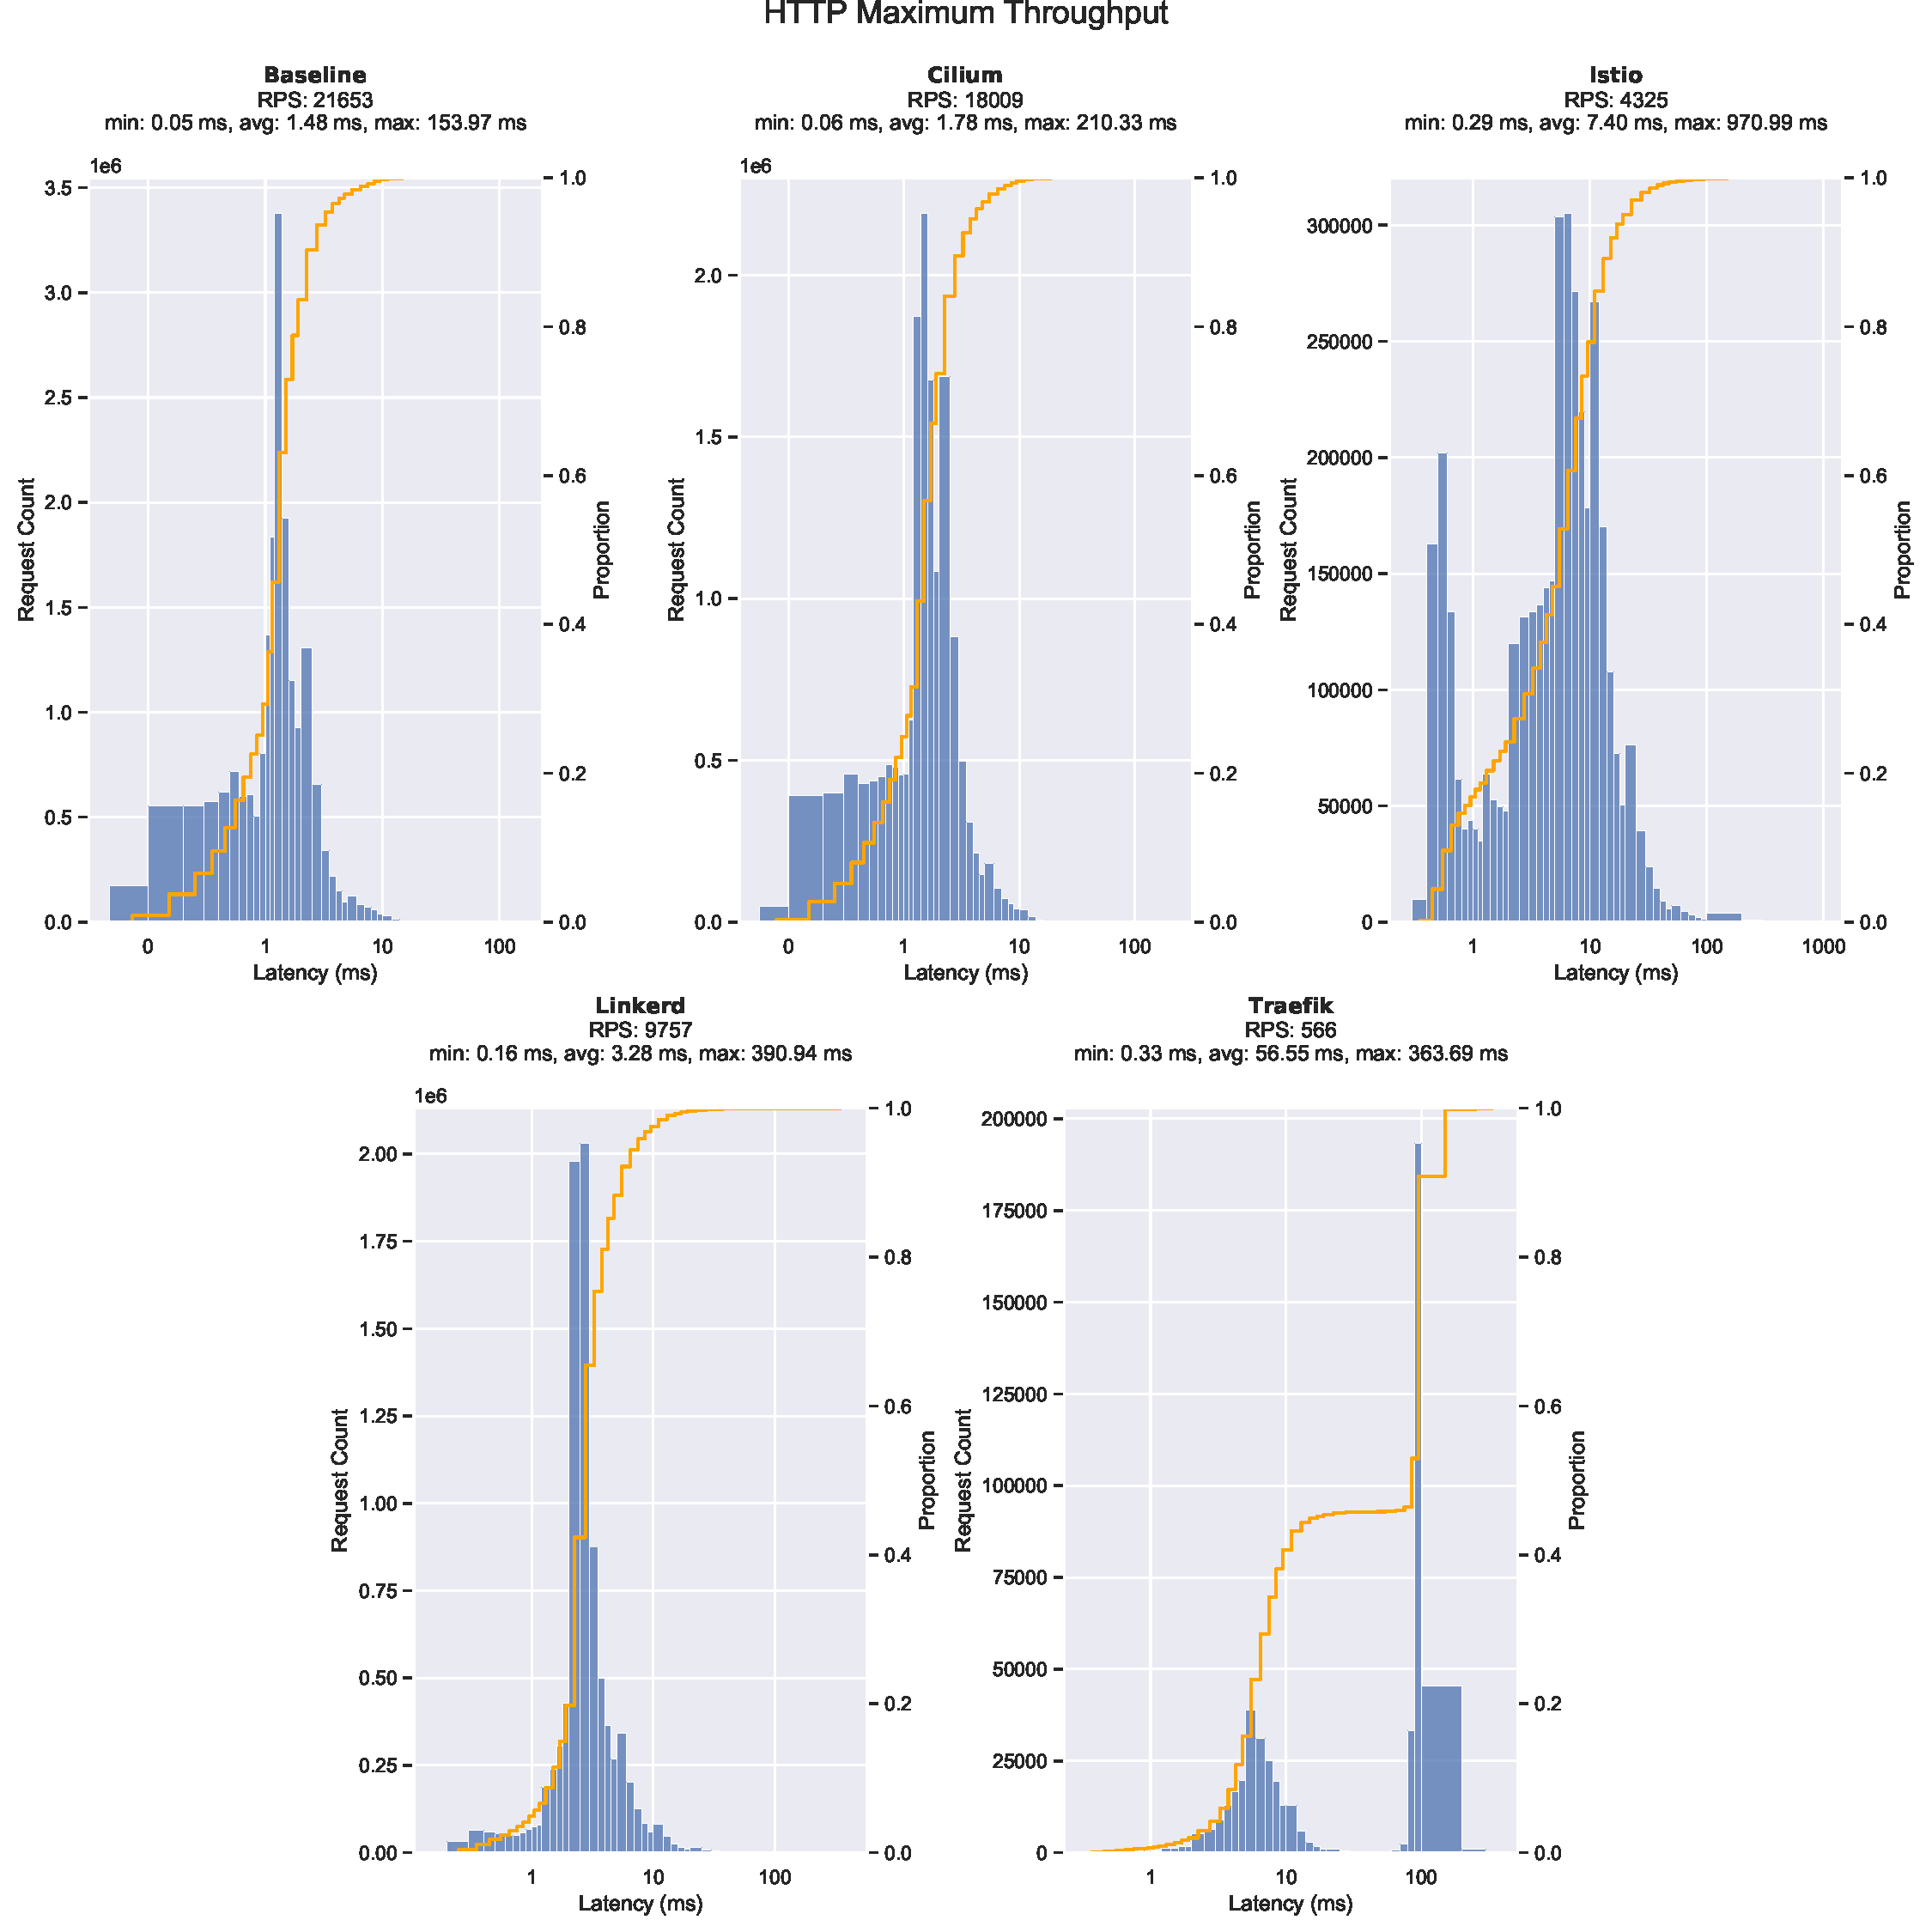
\includegraphics[width=\linewidth]{5_experimental_evaluation/figures/exp_01-latency-results.pdf}

    \caption{\ref{exp:design:1} - Latency Results}
    
    \label{fig:exp:result:01:latency}
\end{figure}



% Findings
% - Baseline best (highest RPS, best latency avg)
% - Distributions roughly normal
% - Large increases in average/tail end latencies
% - Traefik mesh bimodal distribution
% cilium QPS diff: -16.827679769486704%
% istio QPS diff: -80.0264142981776%
% linkerd QPS diff: -54.940993873502805%
% traefik QPS diff: -97.38692130213765%
From the histograms in \cref{fig:exp:result:01:latency} we can observe that the baseline performs the best, i.e. it has the highest observed throughput and the minimum, average and maximum latencies outperform any meshed configuration. In terms of achieved throughput, \textit{Cilium} performs second best and loses $-16.83\%$ compared to the baseline configuration with no \gls{sm} applied. The configuration using \textit{Linkerd}, however, lost more than half ($-54.94\%$), whereas the situation for \textit{Istio} and \textit{Traefik} was even worse as they saw a throughput drop of $-80.26\%$ and $-97.39\%$ respectively. Another interesting observation can be made when looking at the average latencies and tail end latencies for the meshed configurations compared to the baseline measurements. First, we can see a minor increase in average latency for \textit{Cilium}. More interestingly, however, we can see a $+121.62\%$ increase for the \textit{Linkerd} configuration compared to the baseline. The results for the \textit{Istio} configuration is even worse, where it sees an uplift of $+400\%$ for the average request latency compared to the baseline. \textit{Traefik}, however, sees the largest increase with a massive $+3720.95\%$ uplift in average request latency. When taking a closer look at the distributions in the histograms we can also notice that the configuration using the \textit{Traefik} mesh has a bimodal distribution, where one mode is around 8 milliseconds and another mode exists around the 100 millisecond mark.

% Explanation CPU/Mem line plots
In \cref{fig:exp:result:01:cpu} and \cref{fig:exp:result:01:memory} we depict the CPU and memory utilization results of the experiment. Both illustrations come in the form of line plots that have their metric expressed on the y-axis, for the CPU usage this is represented as fractions of a CPU core for both user and kernel time and for the memory utilization this is expressed in kilobytes used. On the x-axis we depict the time delta of the experiment since the start in minutes, each experiment takes 15 minutes and the lines in the plot show the resource utilization values over time. Additionally, each plot can have multiple lines, with one line for each container relevant to the configuration. In other words, we track the resource utilization for the containers related to the data path of the network traffic. In the baseline configuration this is only one experiment, since it does not employ a \gls{sm}, but in the meshed configurations proxy containers are plotted as well as indicated by the legends above the figures.

\begin{figure}[!t]
    \centering
    
    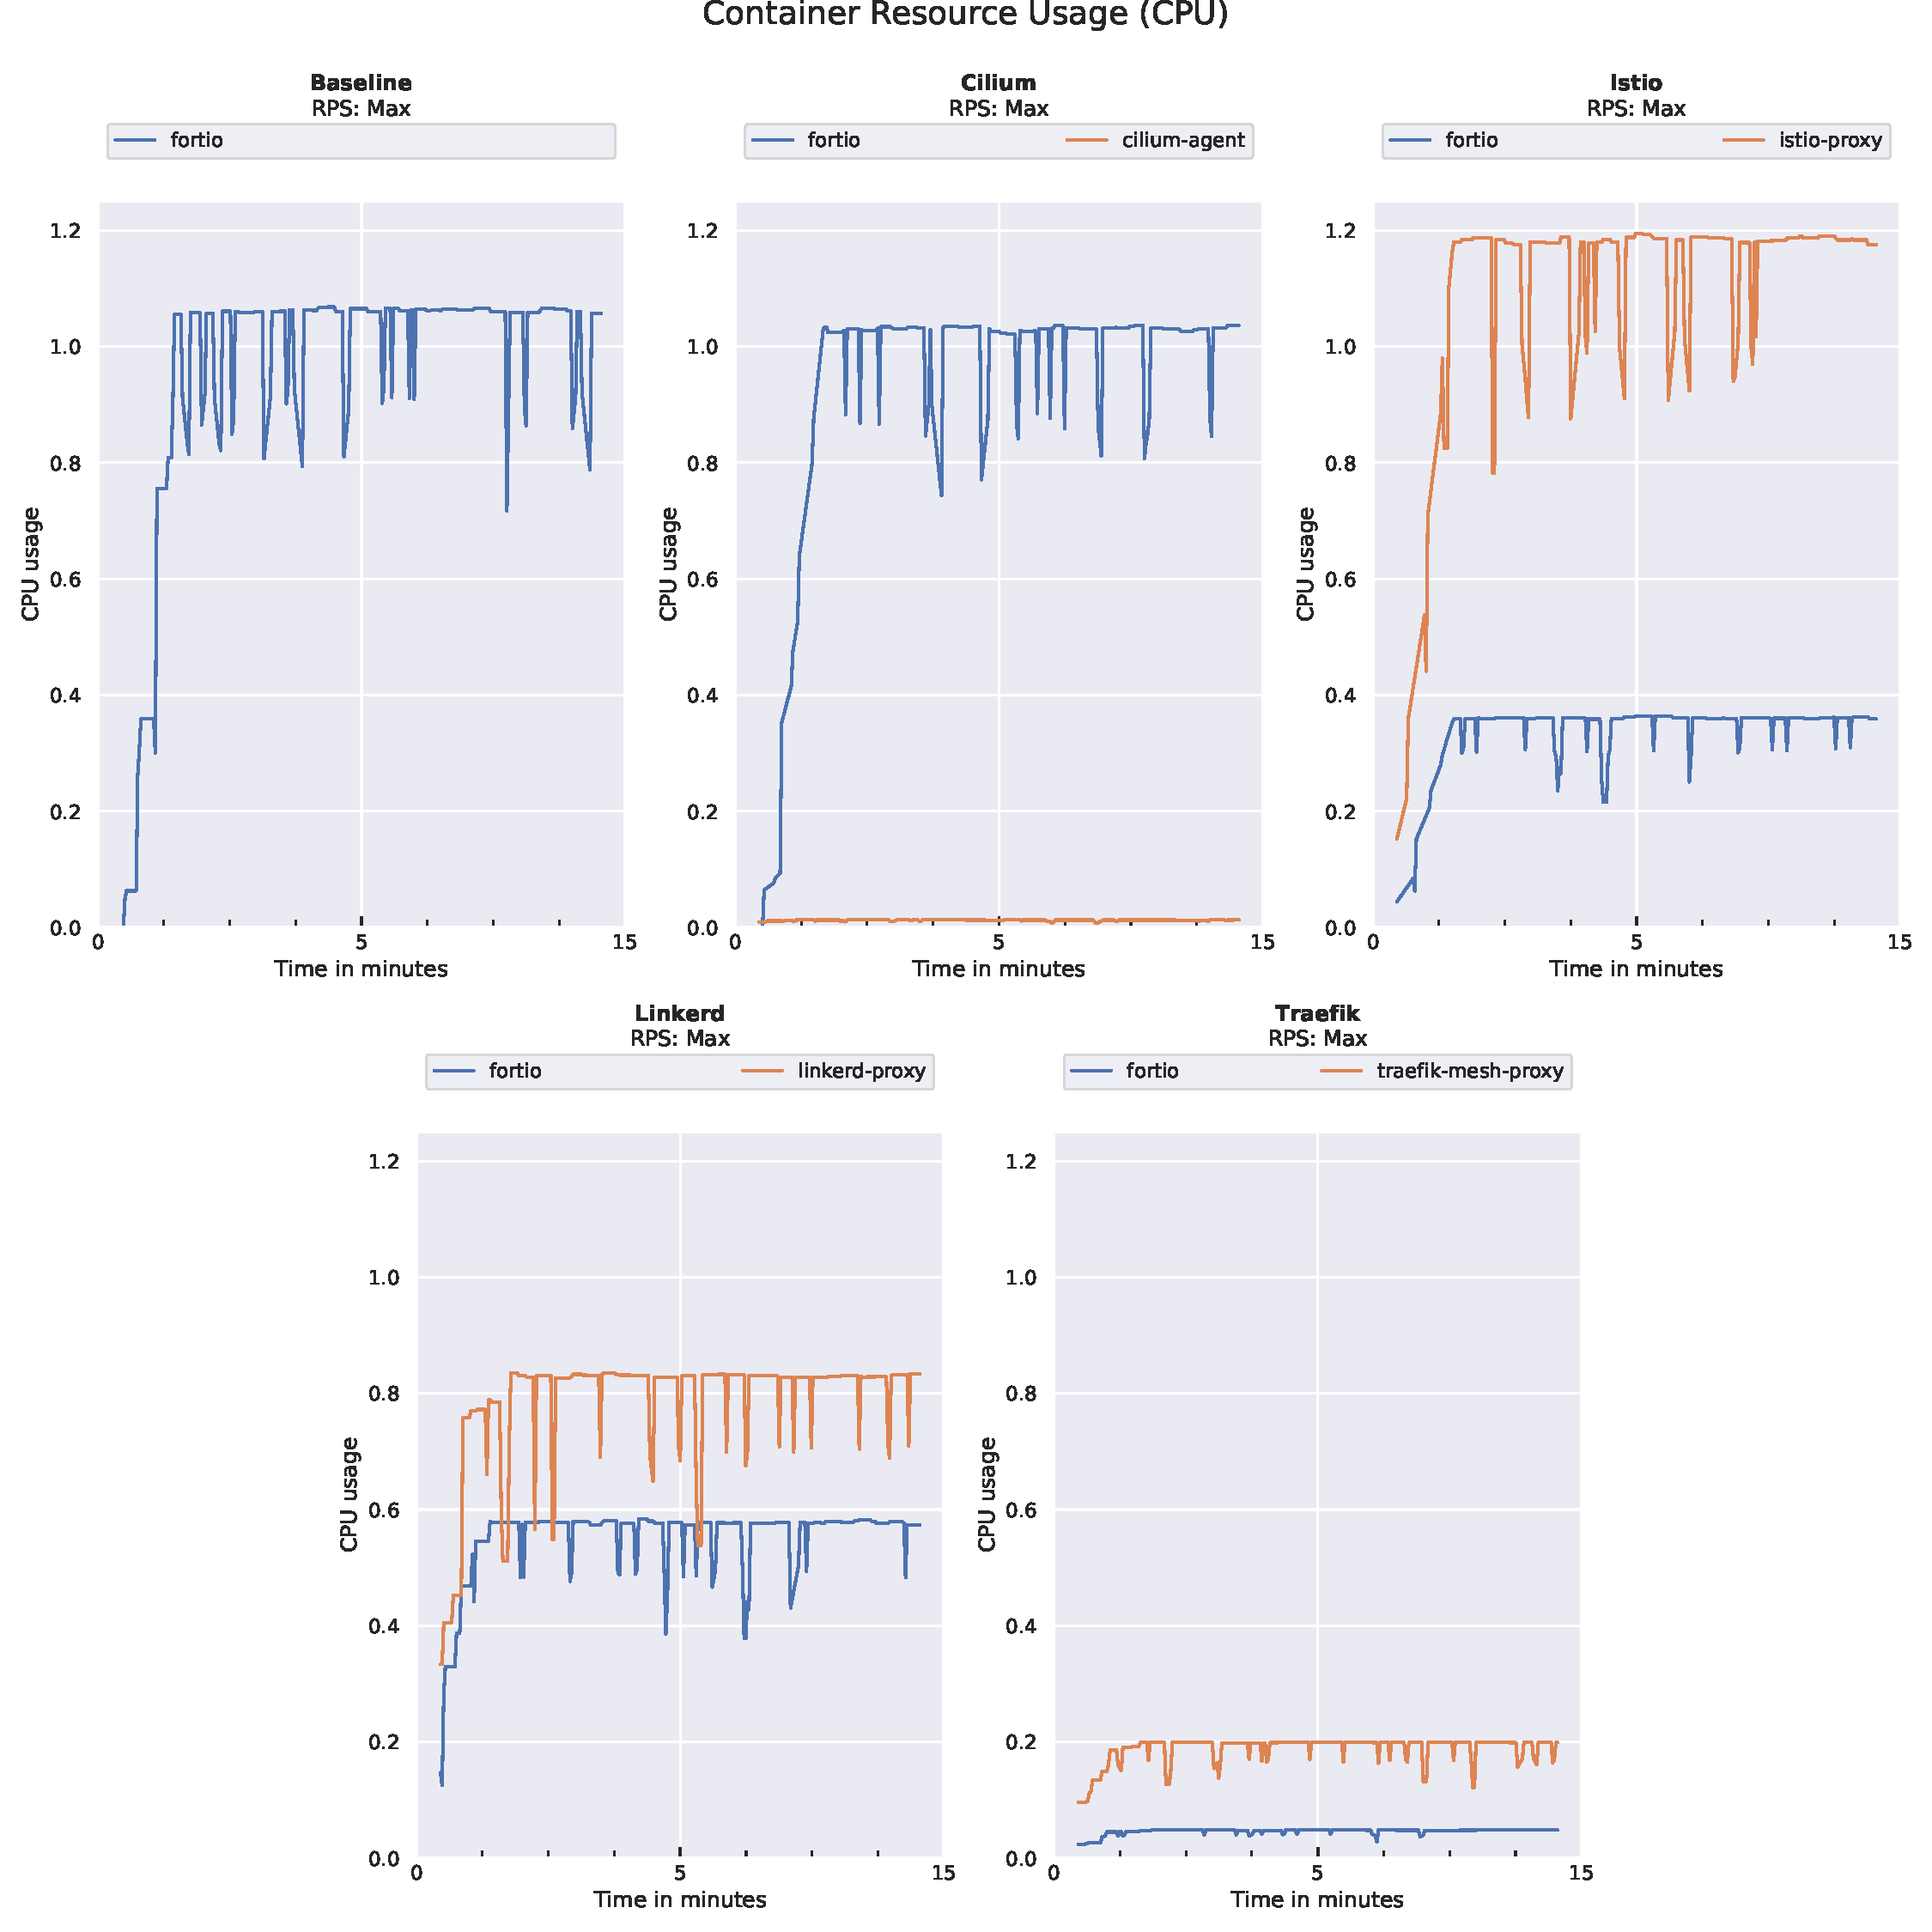
\includegraphics[width=\linewidth]{5_experimental_evaluation/figures/exp_01-cpu-results.pdf}

    \caption{\ref{exp:design:1} - CPU utilization results.}
    
    \label{fig:exp:result:01:cpu}
\end{figure}


% Notable findings
% Small rampup time
% 'fortio' usage -> RPS
% Istio-proxy high utilization
% Linkerd less, but more throughput
% Cilium very low utilization
% Traefik low -> bottleneck?
From the line plots in \cref{fig:exp:result:01:cpu} we can observe that for each configuration there is a small ramp-up time until the CPU utilization settles in. Furthermore, we can observe and relate back to our results depicted in the histograms (\cref{fig:exp:result:01:latency}) that there is a direct correlation between CPU utilization and throughput for the \textit{fortio} container (the target service that represents an echo server), as the meshed configurations that achieved less throughput have an inverse relation on CPU utilization. Interesting observations can be made regarding the CPU utilization of the service proxies. First of, \textit{Cilium}, with their kernel based proxying solution (\cref{{sec:survey:results:comparison:proxy}}) seems to have very little overhead compared to other proxying solutions. Second, the proxy used in the \textit{Istio} configuration appears to have the highest overhead, taking up more than an entire CPU core. Additionally, the proxy used in the \textit{Linkerd} configuration uses less CPU resources, which indicates that this solution is more efficient than \textit{Linkerd}'s proxy as it was able to handle a higher throughput as well. Finally, we observe that the \textit{Traefik} configuration used very CPU little resources at all, indicating bottlenecks of some sort.

From the plots depicting memory consumption in \cref{fig:exp:result:01:memory} we can see that for each configuration the memory usage was very minimal. The \textit{cilium-agent} container reached a spike and consumed at most $2.27$MB during maximum load. This amount is negligible for most systems and indicates that the data path proxies will likely not be memory constrained.

\begin{figure}[!t]
    \centering
    
    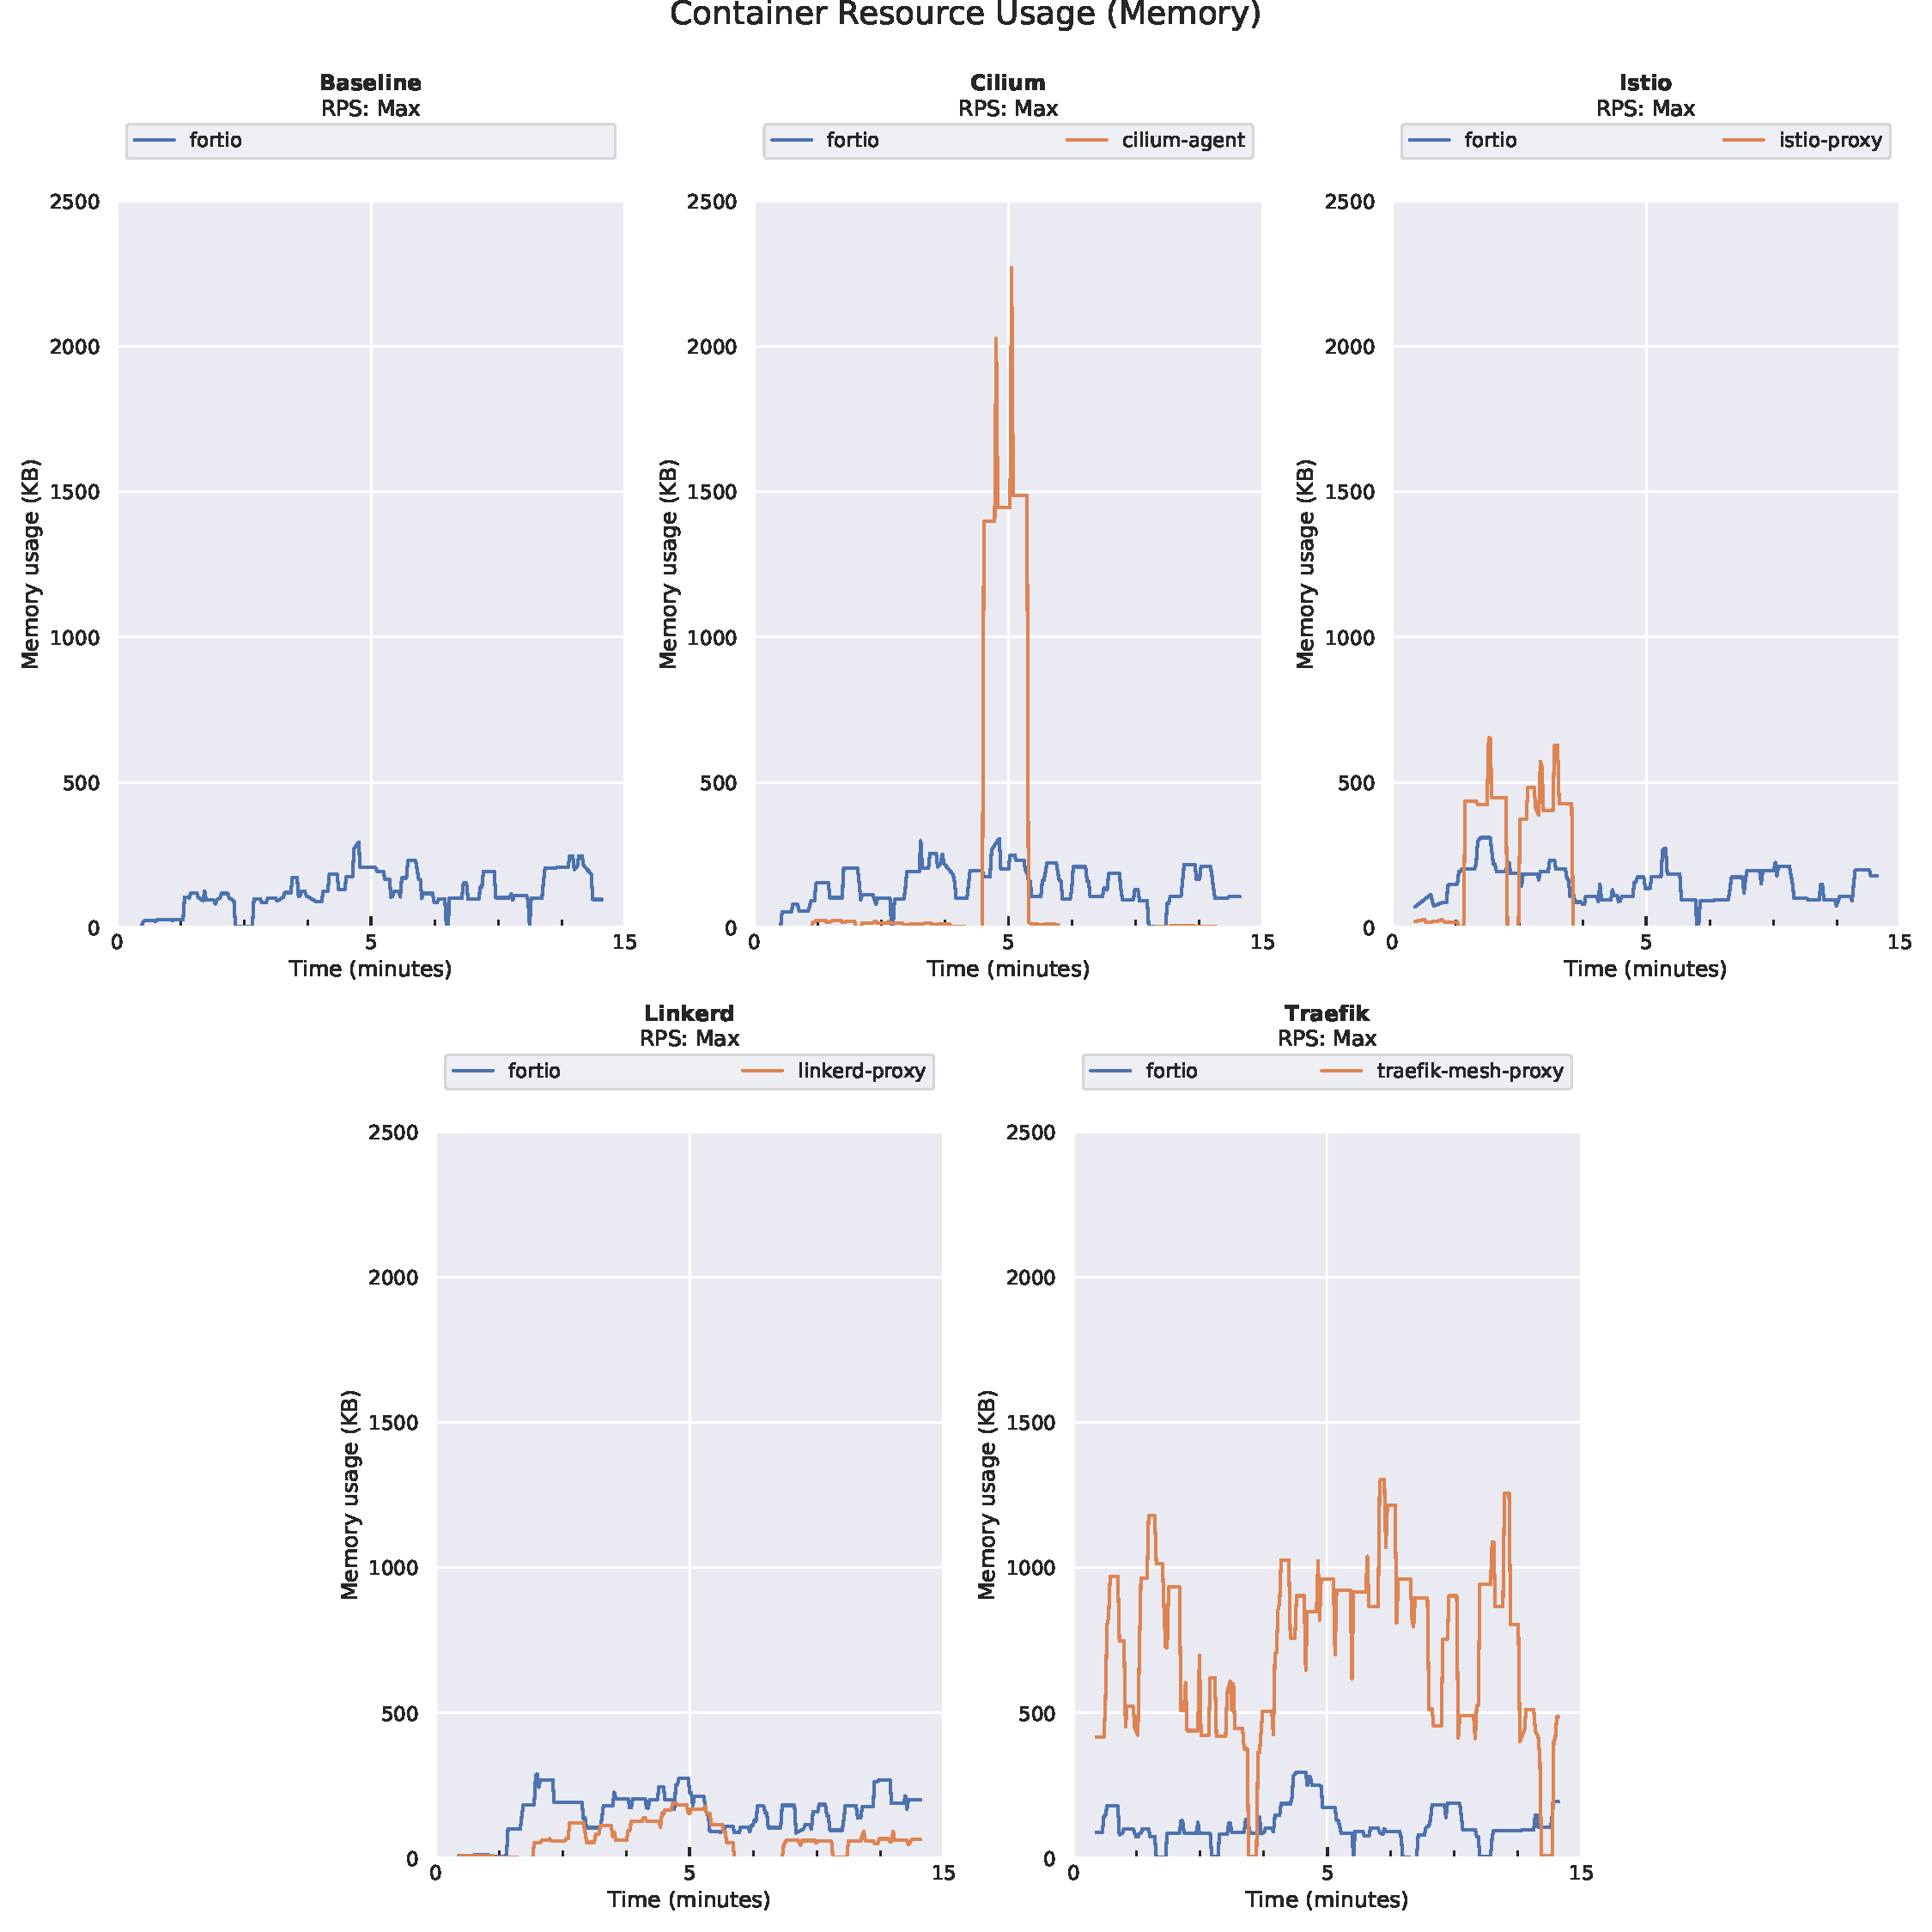
\includegraphics[width=\linewidth]{5_experimental_evaluation/figures/exp_01-memory-results.pdf}

    \caption{\ref{exp:design:1} - Memory Results}
    
    \label{fig:exp:result:01:memory}
\end{figure}



\subsubsection{\ref{exp:design:2} - HTTP Constant Throughput}
\label{sec:experiments:results:per-experiment:02}
% Goal: To evaluate how \gls{sm} configurations behave under varying levels of load.

The second experiment had as goal to evaluate the different \gls{sm} configurations under predefined levels of constant throughput. The results of this experiment are depicted in \cref{fig:exp:result:02:latency}, \cref{fig:exp:result:02:cpu} and \label{fig:exp:result:02:memory}.


\begin{figure}[!t]
    \centering
    
    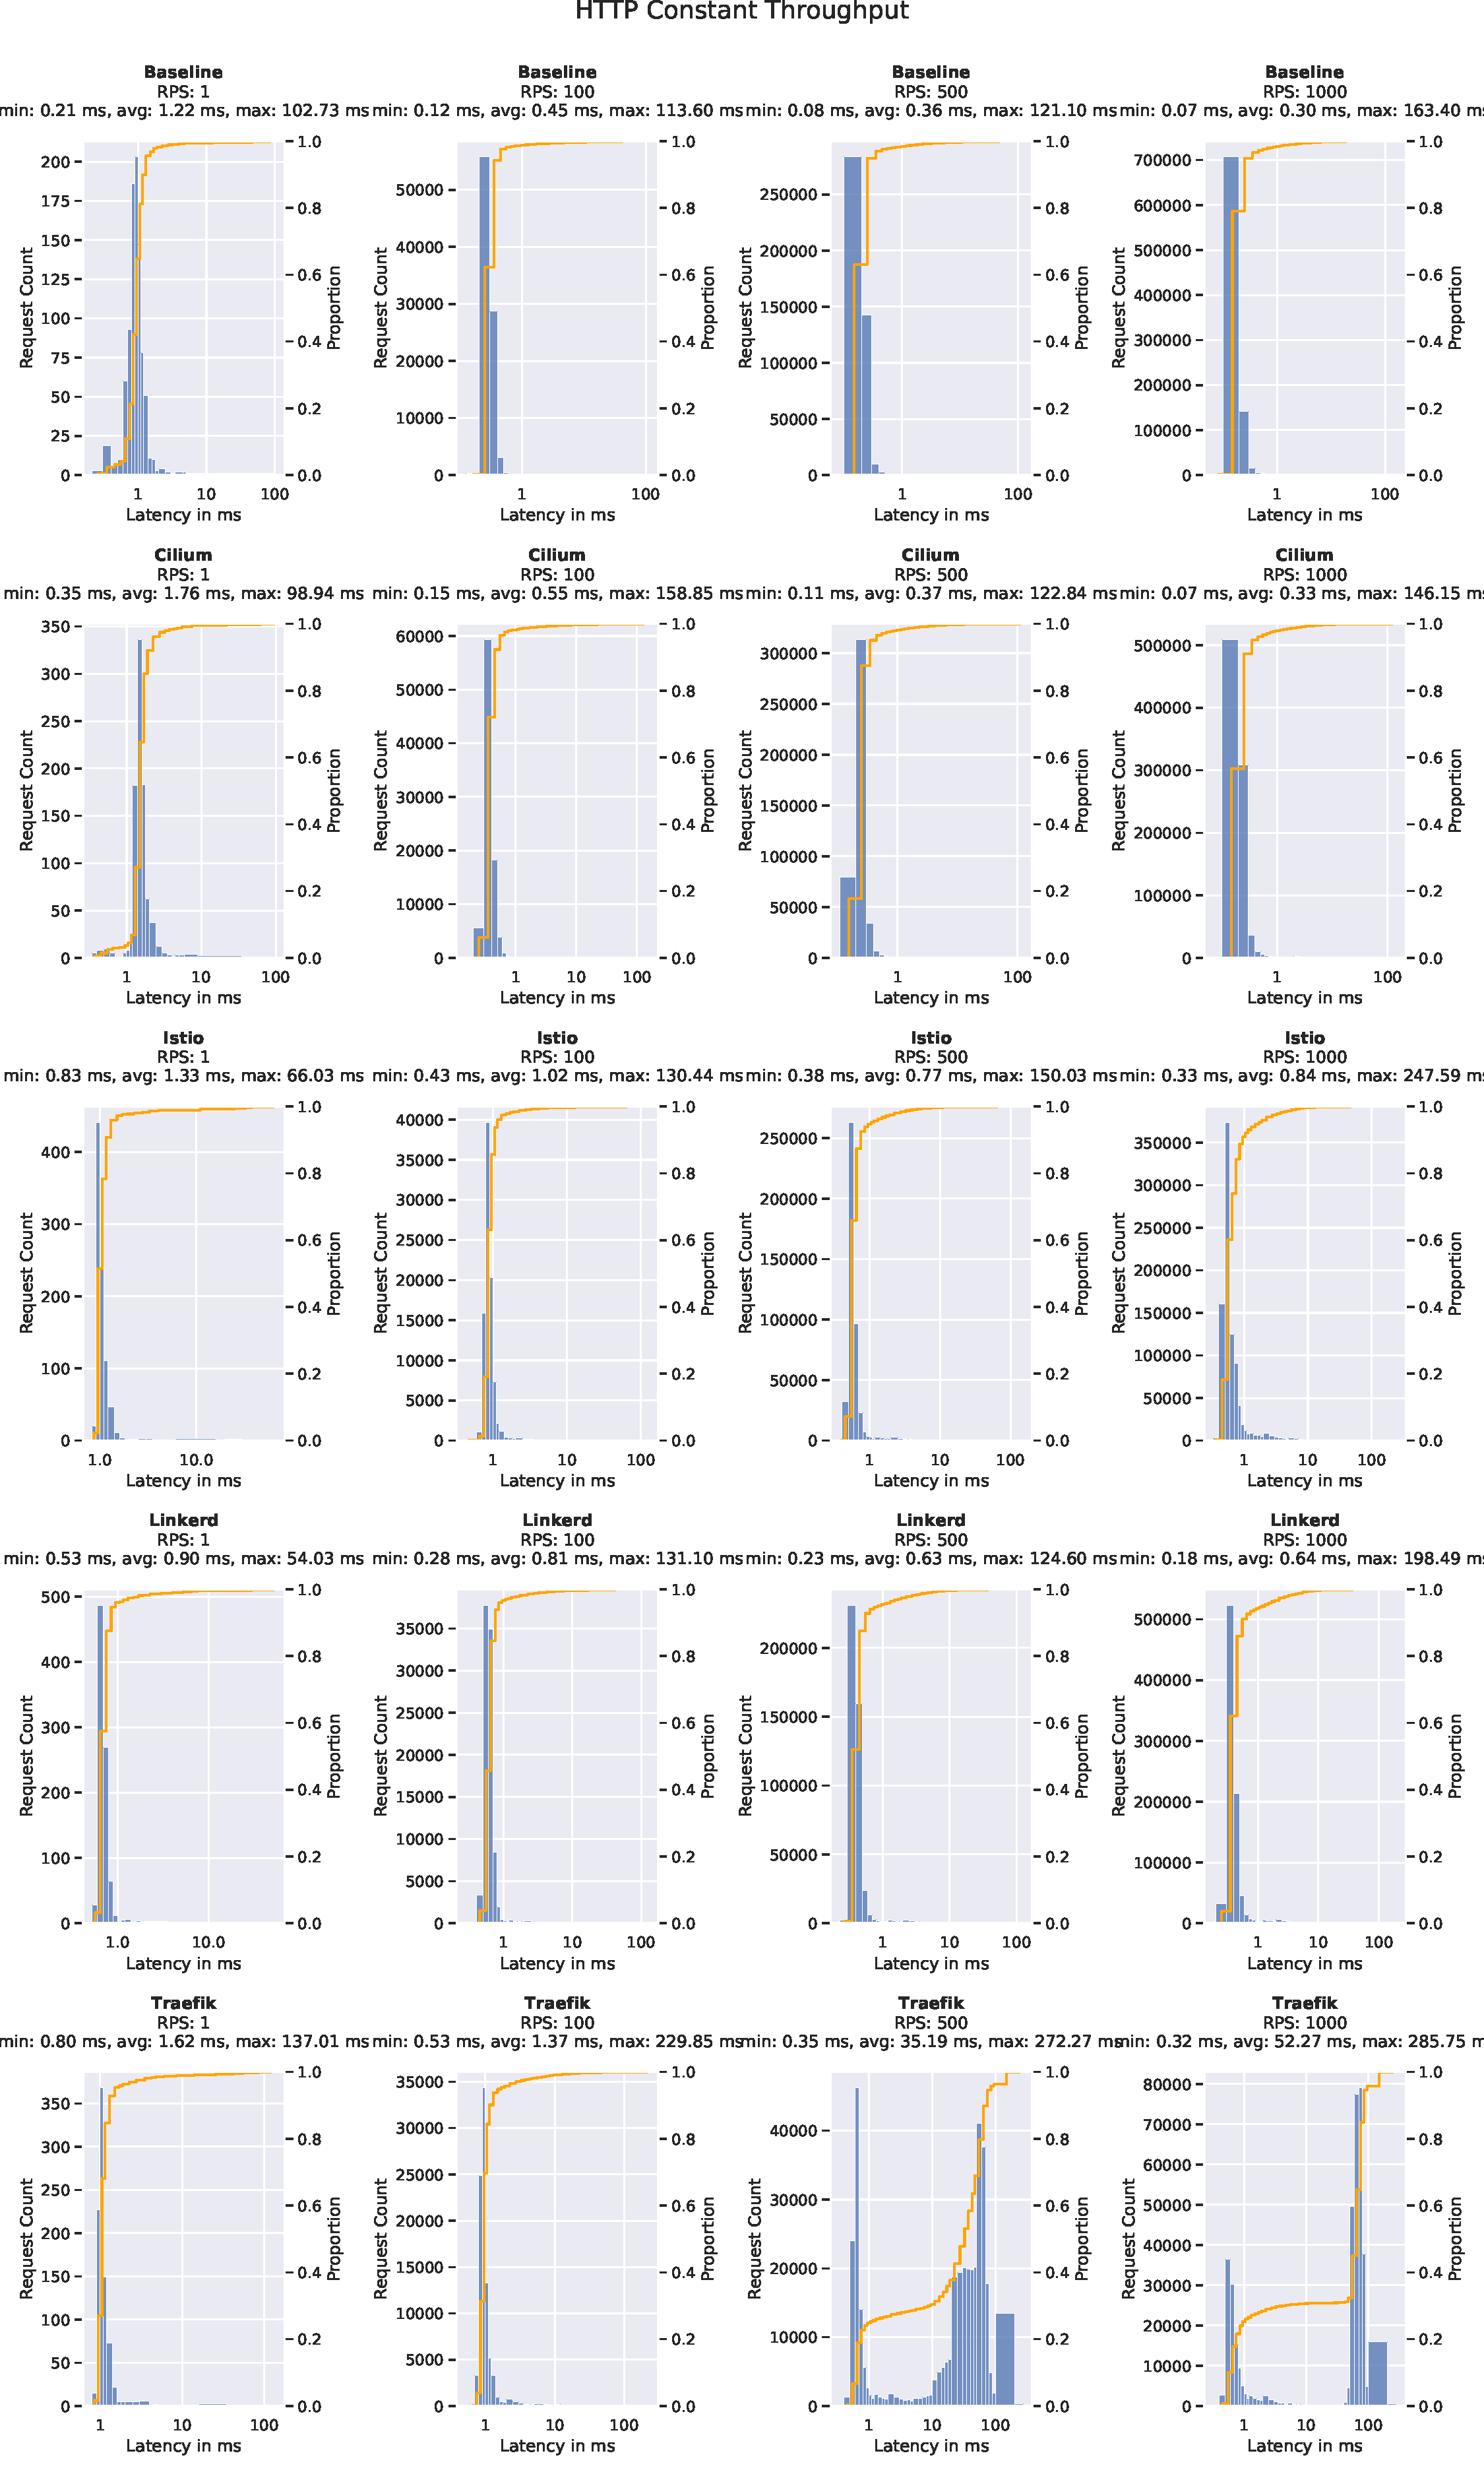
\includegraphics[width=\textwidth,height=\textheight]{5_experimental_evaluation/figures/exp_02-latency-combined-results-offset.pdf}

    \caption{\ref{exp:design:2} - Latency Results}
    
    \label{fig:exp:result:02:latency}
\end{figure}

% How to read all three figures
% - Histogram (latency)
% - Line plot (cpu/mem)
In \cref{fig:exp:result:02:latency} we present a multitude of histograms that display the request latencies measured in each experiment. Every meshed configuration is presented on a row, where each plot on that row contains the histogram for a certain level of throughput. Again, above each histogram we present descriptive statistics and also plot the cumulative density function. In \cref{fig:exp:result:02:cpu} and \cref{fig:exp:result:02:memory} we present the resource utilization metrics obtained from this experiment. Each plot in the illustrations represents a meshed configuration. The y-axis represents the system resource metric such as CPU or memory utilization. The x-axis represents the time delta since the start of the experiment. Note that the line is continuous, since all four different levels of constant throughput are measured one after another. Additionally, each line is coloured and represents a single container on the data path, i.e. target service and proxy (if applicable).

% Results:
% Distribution of traefik changed when peak is hit (~560RPS as in exp1) to bimodal
% Istio/Linkerd max suffering
% - Underlying data/bins (or log plots) show 99p 99.9p suffering
From the histograms \cref{fig:exp:result:02:latency} we can see that for most configurations the distribution stayed very similar. The most significant difference occurs at \textit{Traefik}, where the bimodal distribution occurs at a constant throughput of 500 requests per second and above. This falls in line with the observed behaviour as experienced in \ref{exp:design:1} and indicates a bottleneck of some sort. We can also observe from the descriptive statistics that the maximum values observed in these controlled environments seem to suffer for \textit{Istio}, \textit{Linkerd} and \textit{Traefik} which can be confirmed by taking a closer look at the underlying data that shows higher latency outliers in the tail ends of the spectrum in the 99th and 99.9th percentile.


\begin{figure}[h]
    \centering
    
    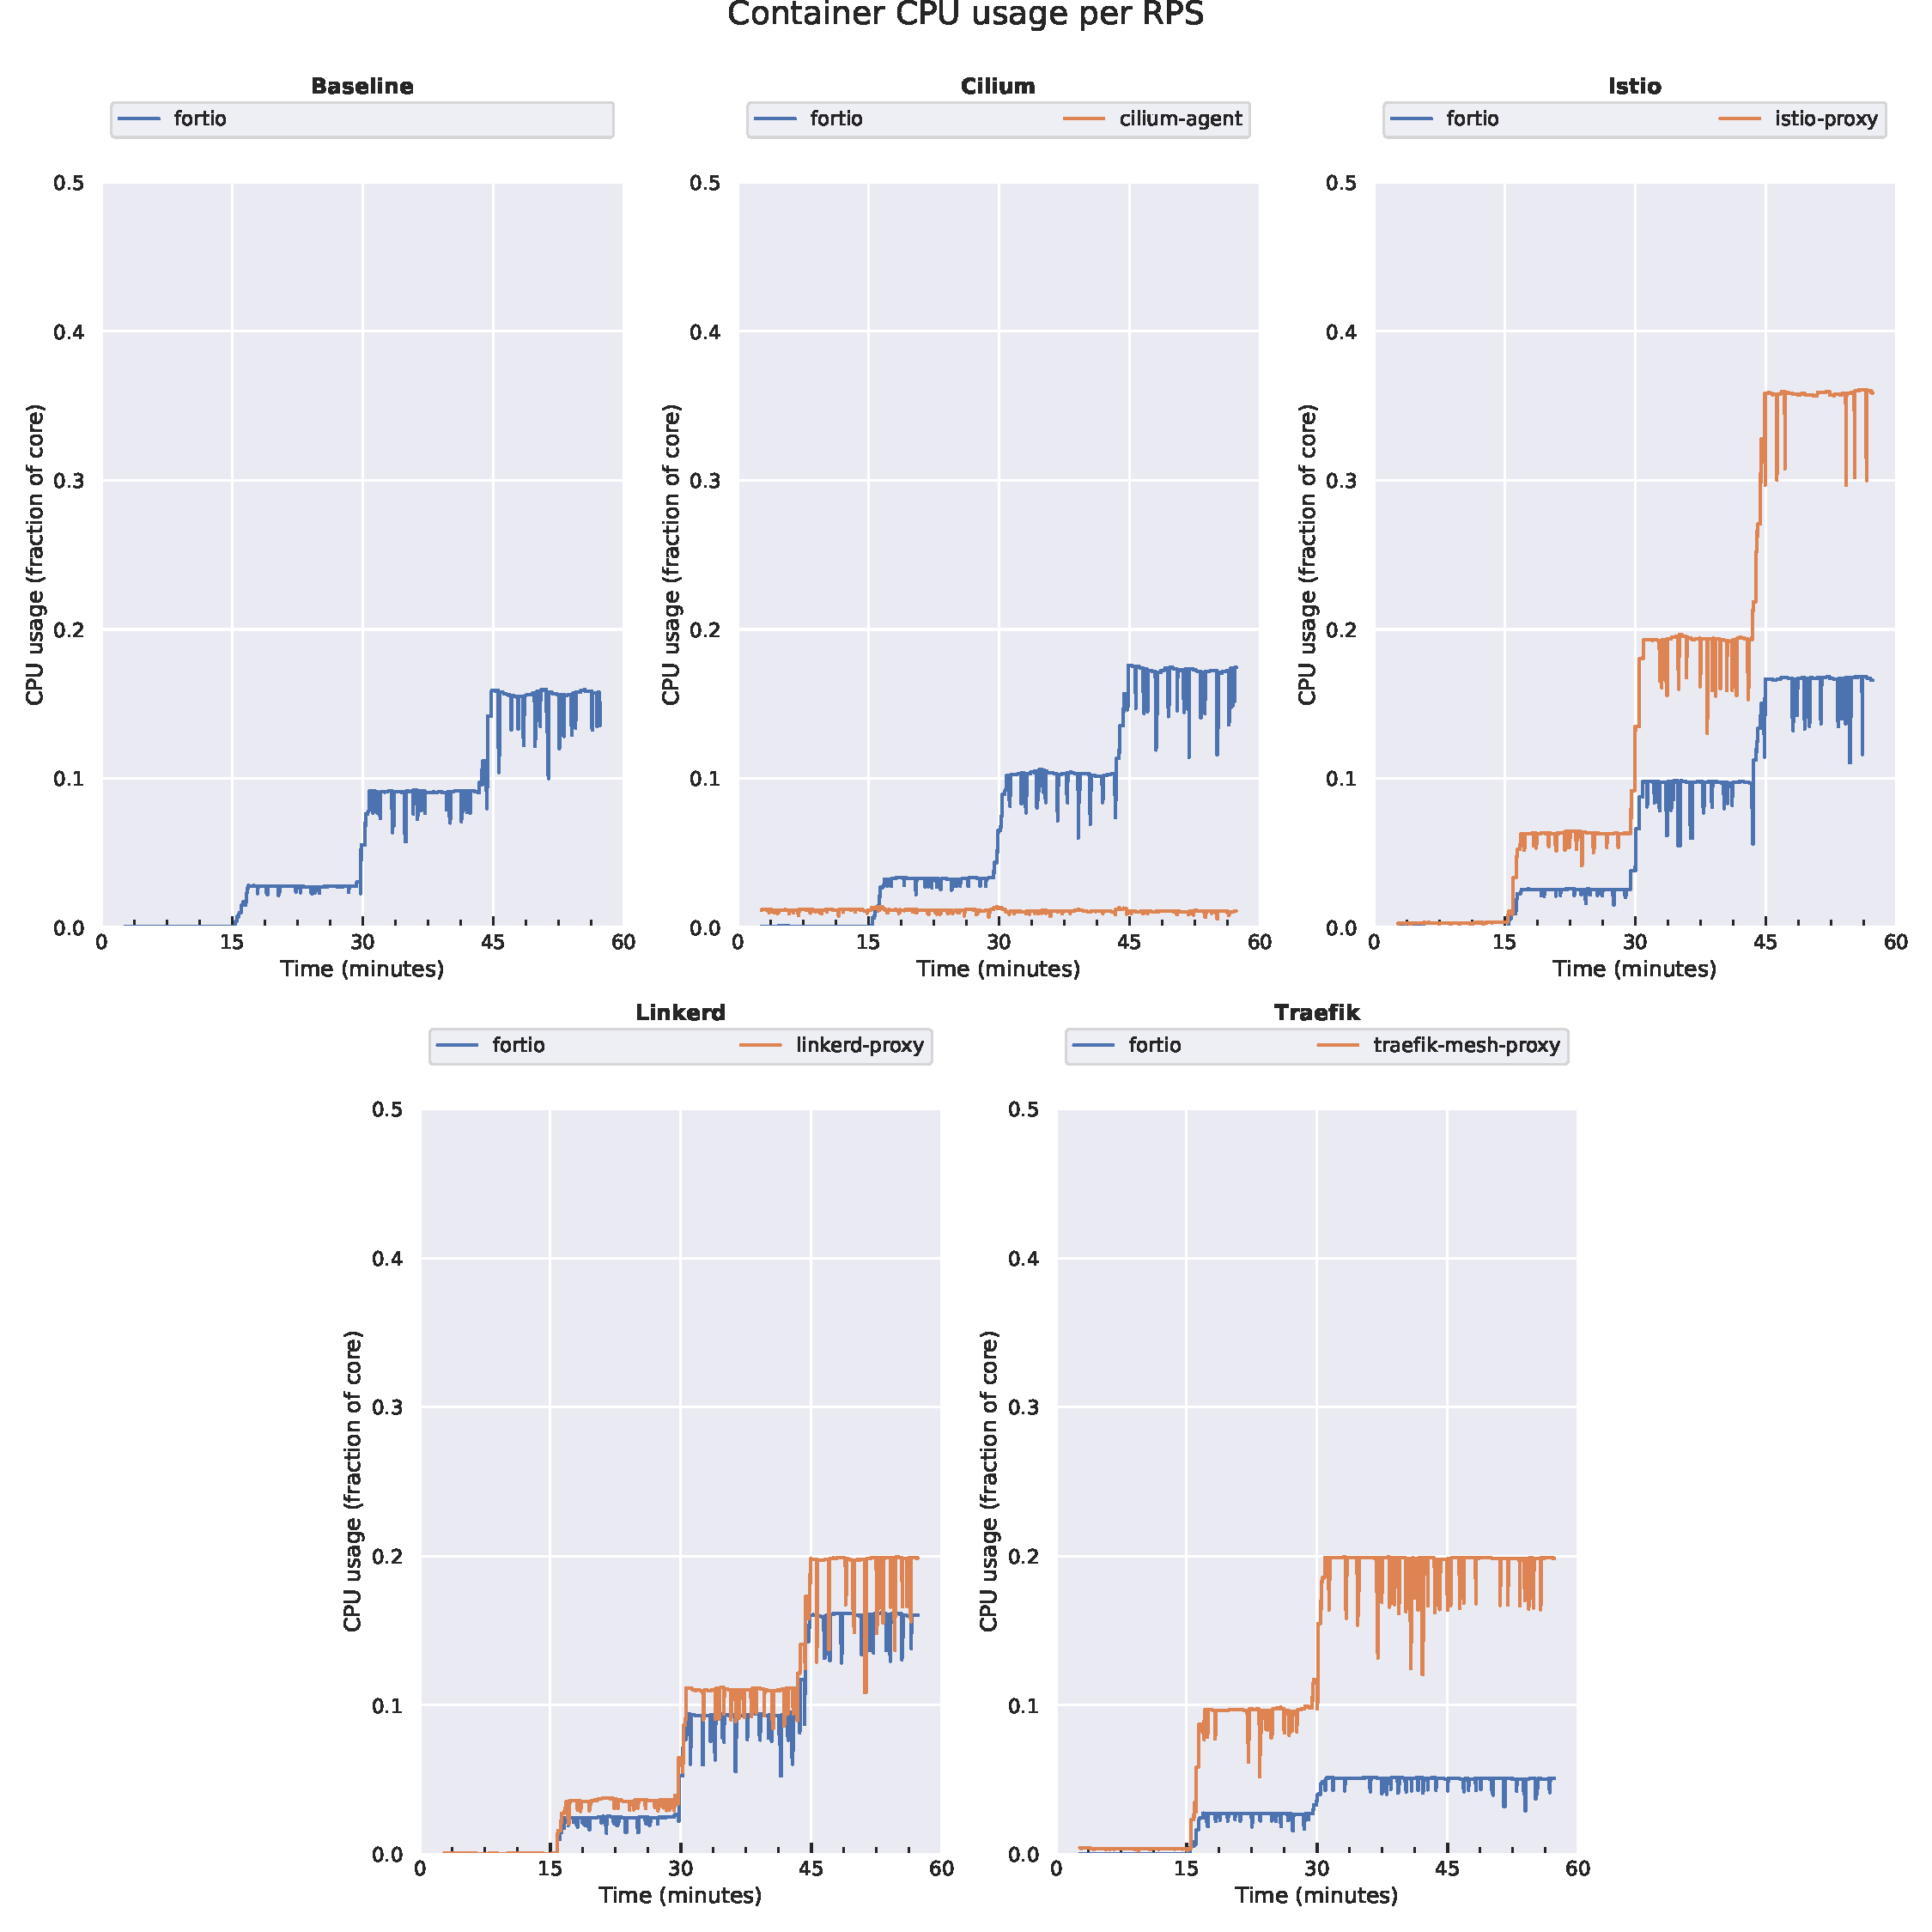
\includegraphics[width=\linewidth]{5_experimental_evaluation/figures/exp_02-cpu-results.pdf}

    \caption{\ref{exp:design:2} - CPU utilization results.}
    
    \label{fig:exp:result:02:cpu}
\end{figure}


% Linar scaling of CPU utilization service
% Istio worst scaling
% Traefik bottleneck at 500
% Memory consumtion similar at all levels
% Linkerd least amount of memory
From the CPU utilization results as depicted in \cref{fig:exp:result:02:cpu} we can observe that the increase in CPU consumption for the target service is linear to the amount of throughput applied. In the results we can observe that \textit{Cilium} seems to consume the least amount of CPU utilization and that it stays stable for each of the workloads. \textit{Istio}, on the other hand, seems to have the worst scaling regarding its CPU utilization. \textit{Linkerd} and \textit{Traefik} seem to scale similarly, however, scaling for the latter stops at the 500 RPS threshold due to its bottleneck. From the memory utilization results as depicted in \cref{fig:exp:result:02:memory} we can observe that \textit{Linkerd} consumes the least amount of memory from all meshed configurations. Another observation is that the memory footprint is similar for each of the workloads, except for the \textit{Traefik} proxy at 1 RPS, which is slightly lower. Again, all observed values are negligible for most environments.


\begin{figure}[h]
    \centering
    
    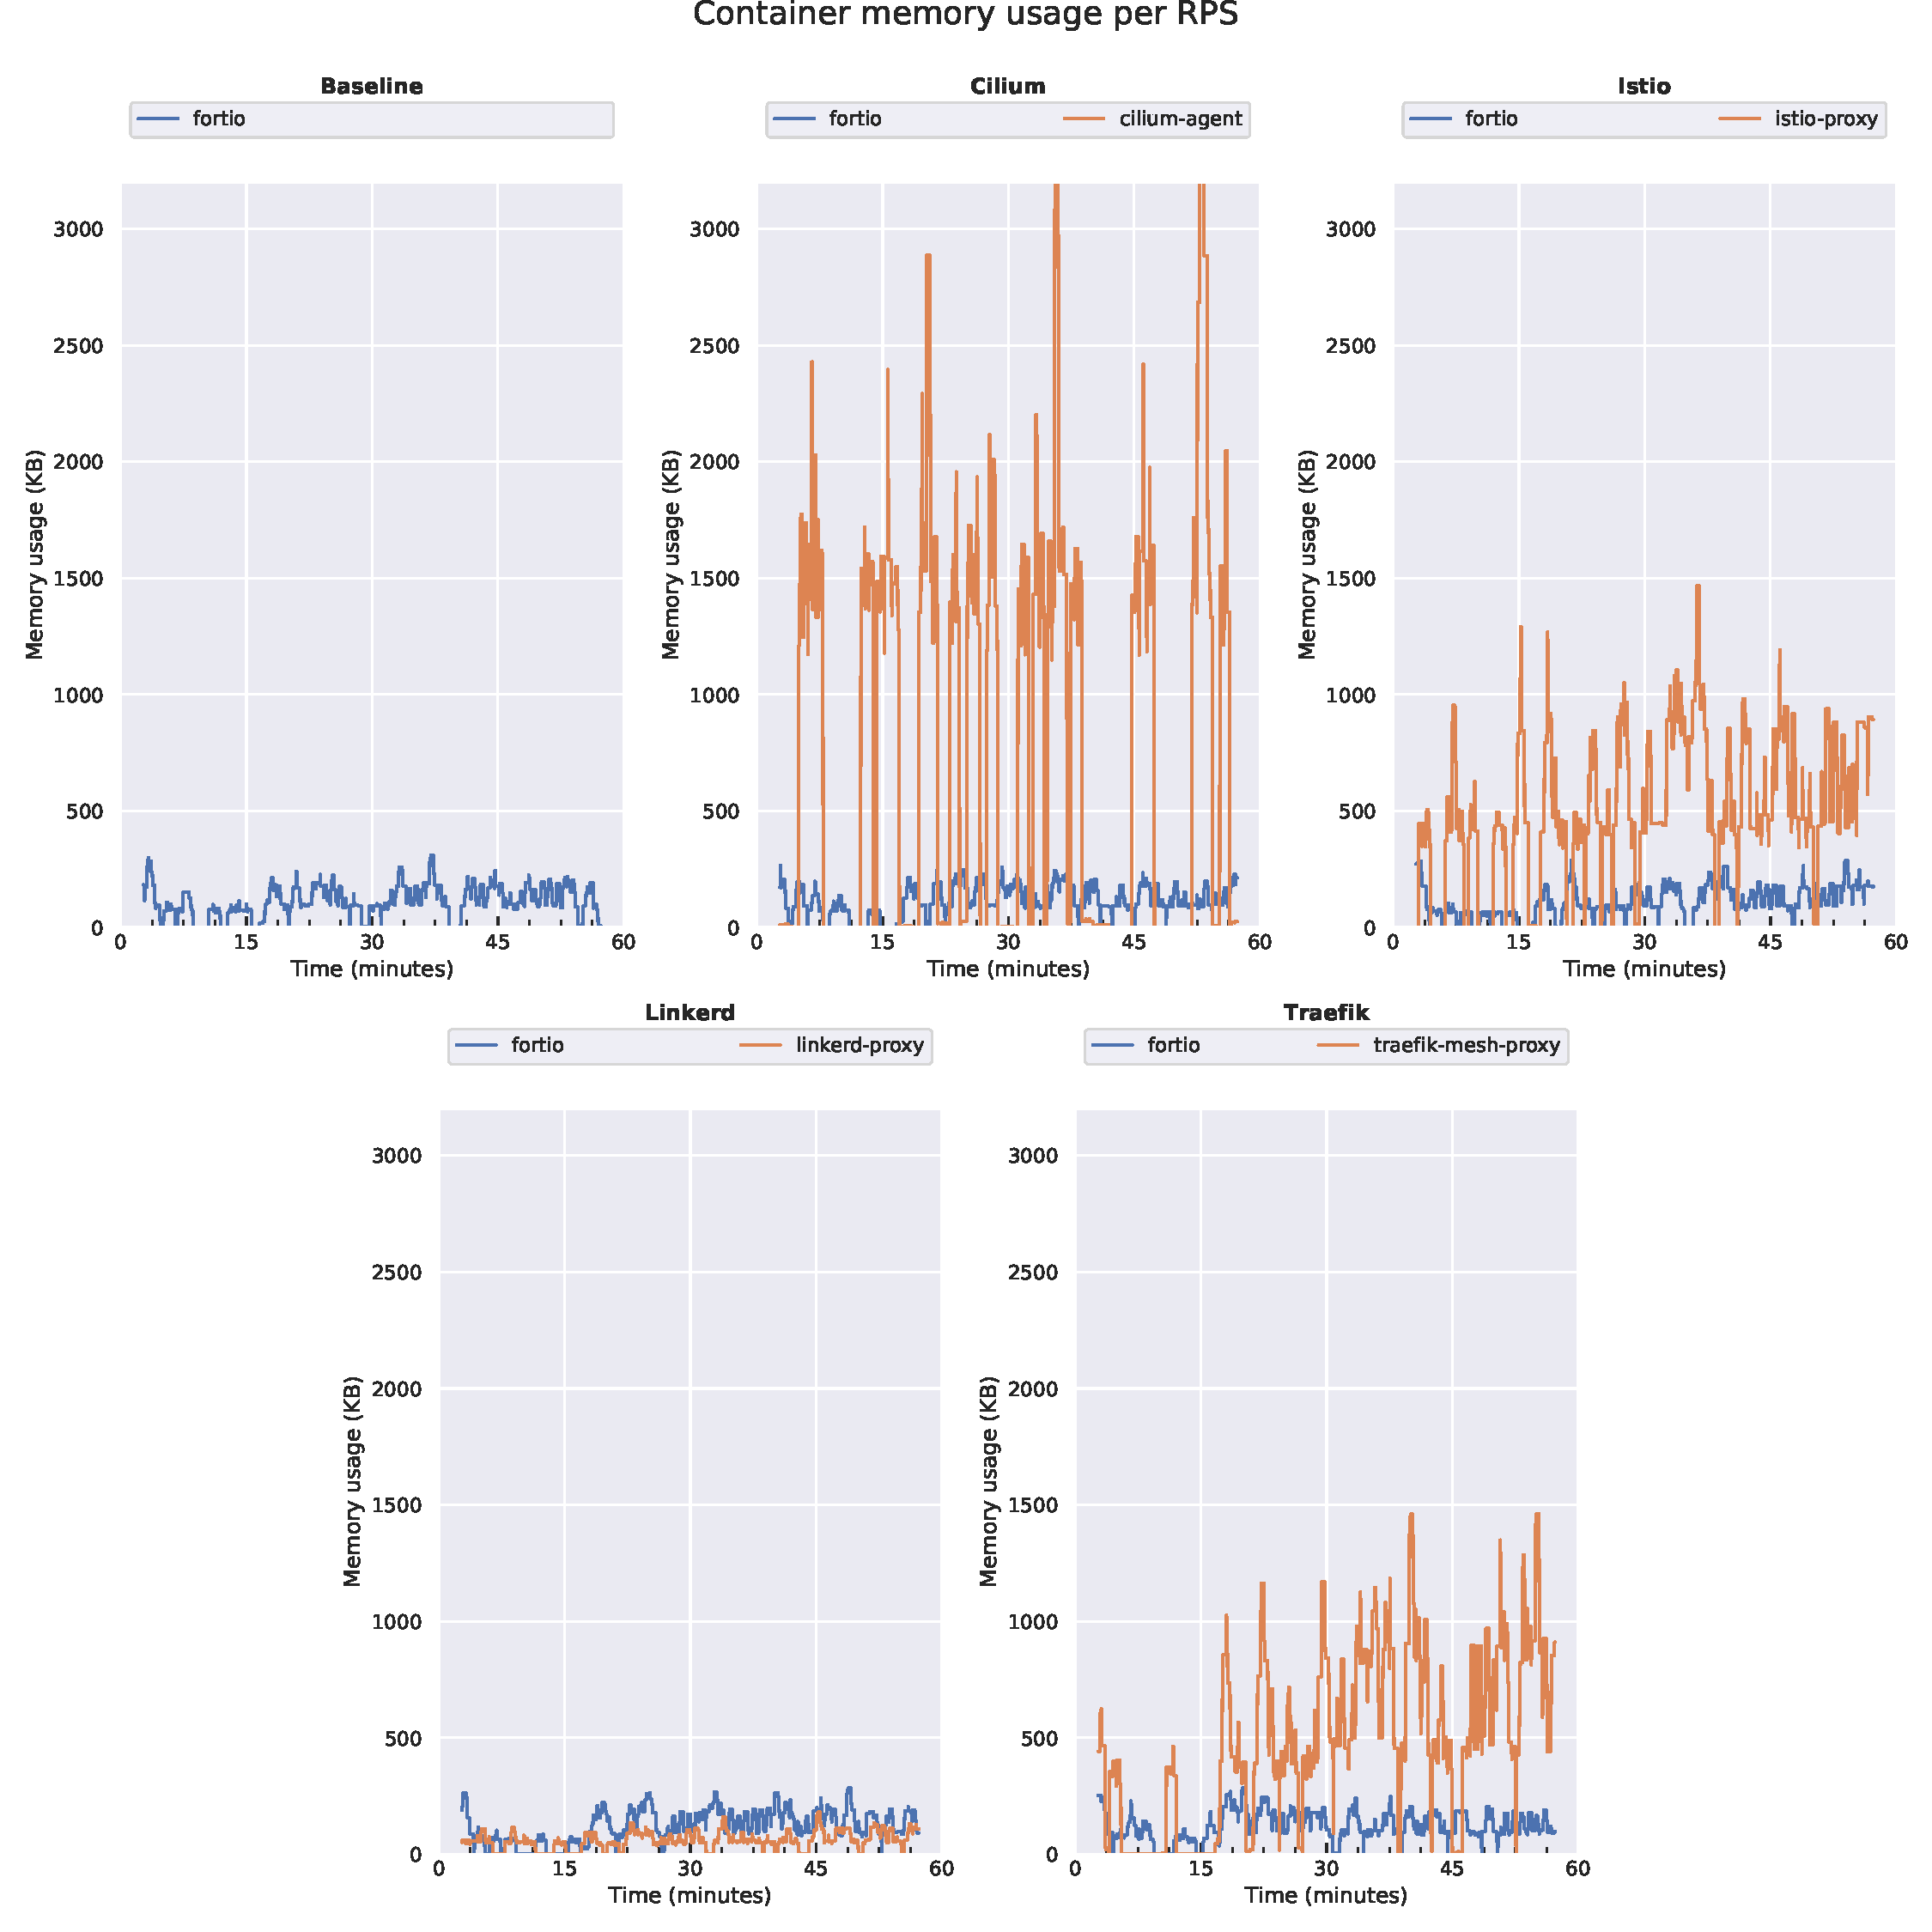
\includegraphics[width=\linewidth]{5_experimental_evaluation/figures/exp_02-mem-results.pdf}

    \caption{\ref{exp:design:2} - memory utilization results.}
    
    \label{fig:exp:result:02:memory}
\end{figure}



\subsubsection{\ref{exp:design:3} - HTTP Payload}
\label{sec:experiments:results:per-experiment:03}

In the third experiment we introduced application payloads. The goal of this experiment is to evaluate the performance of these systems with different payload sizes. The result of this experiment is depicted in \cref{fig:exp:result:03:latency}.

% Explain how to read the figure
\cref{fig:exp:result:03:latency} contains five rows of histogram results. Each of these rows contain the results of a mesh configuration and each of the columns is a result for a given payload size. The first column contains the results of a load test where the target service returns an empty response. The second and third column, however, represent the results of a load test where the target returns a payload of 1 kilobyte and 10 kilobytes respectively as indicated by the plot labels. Additional descriptive statistics are added to each plot without the throughput count as it is static at 100 requests per second for each result in the figure.


\begin{figure}[!t]
    \centering
    
    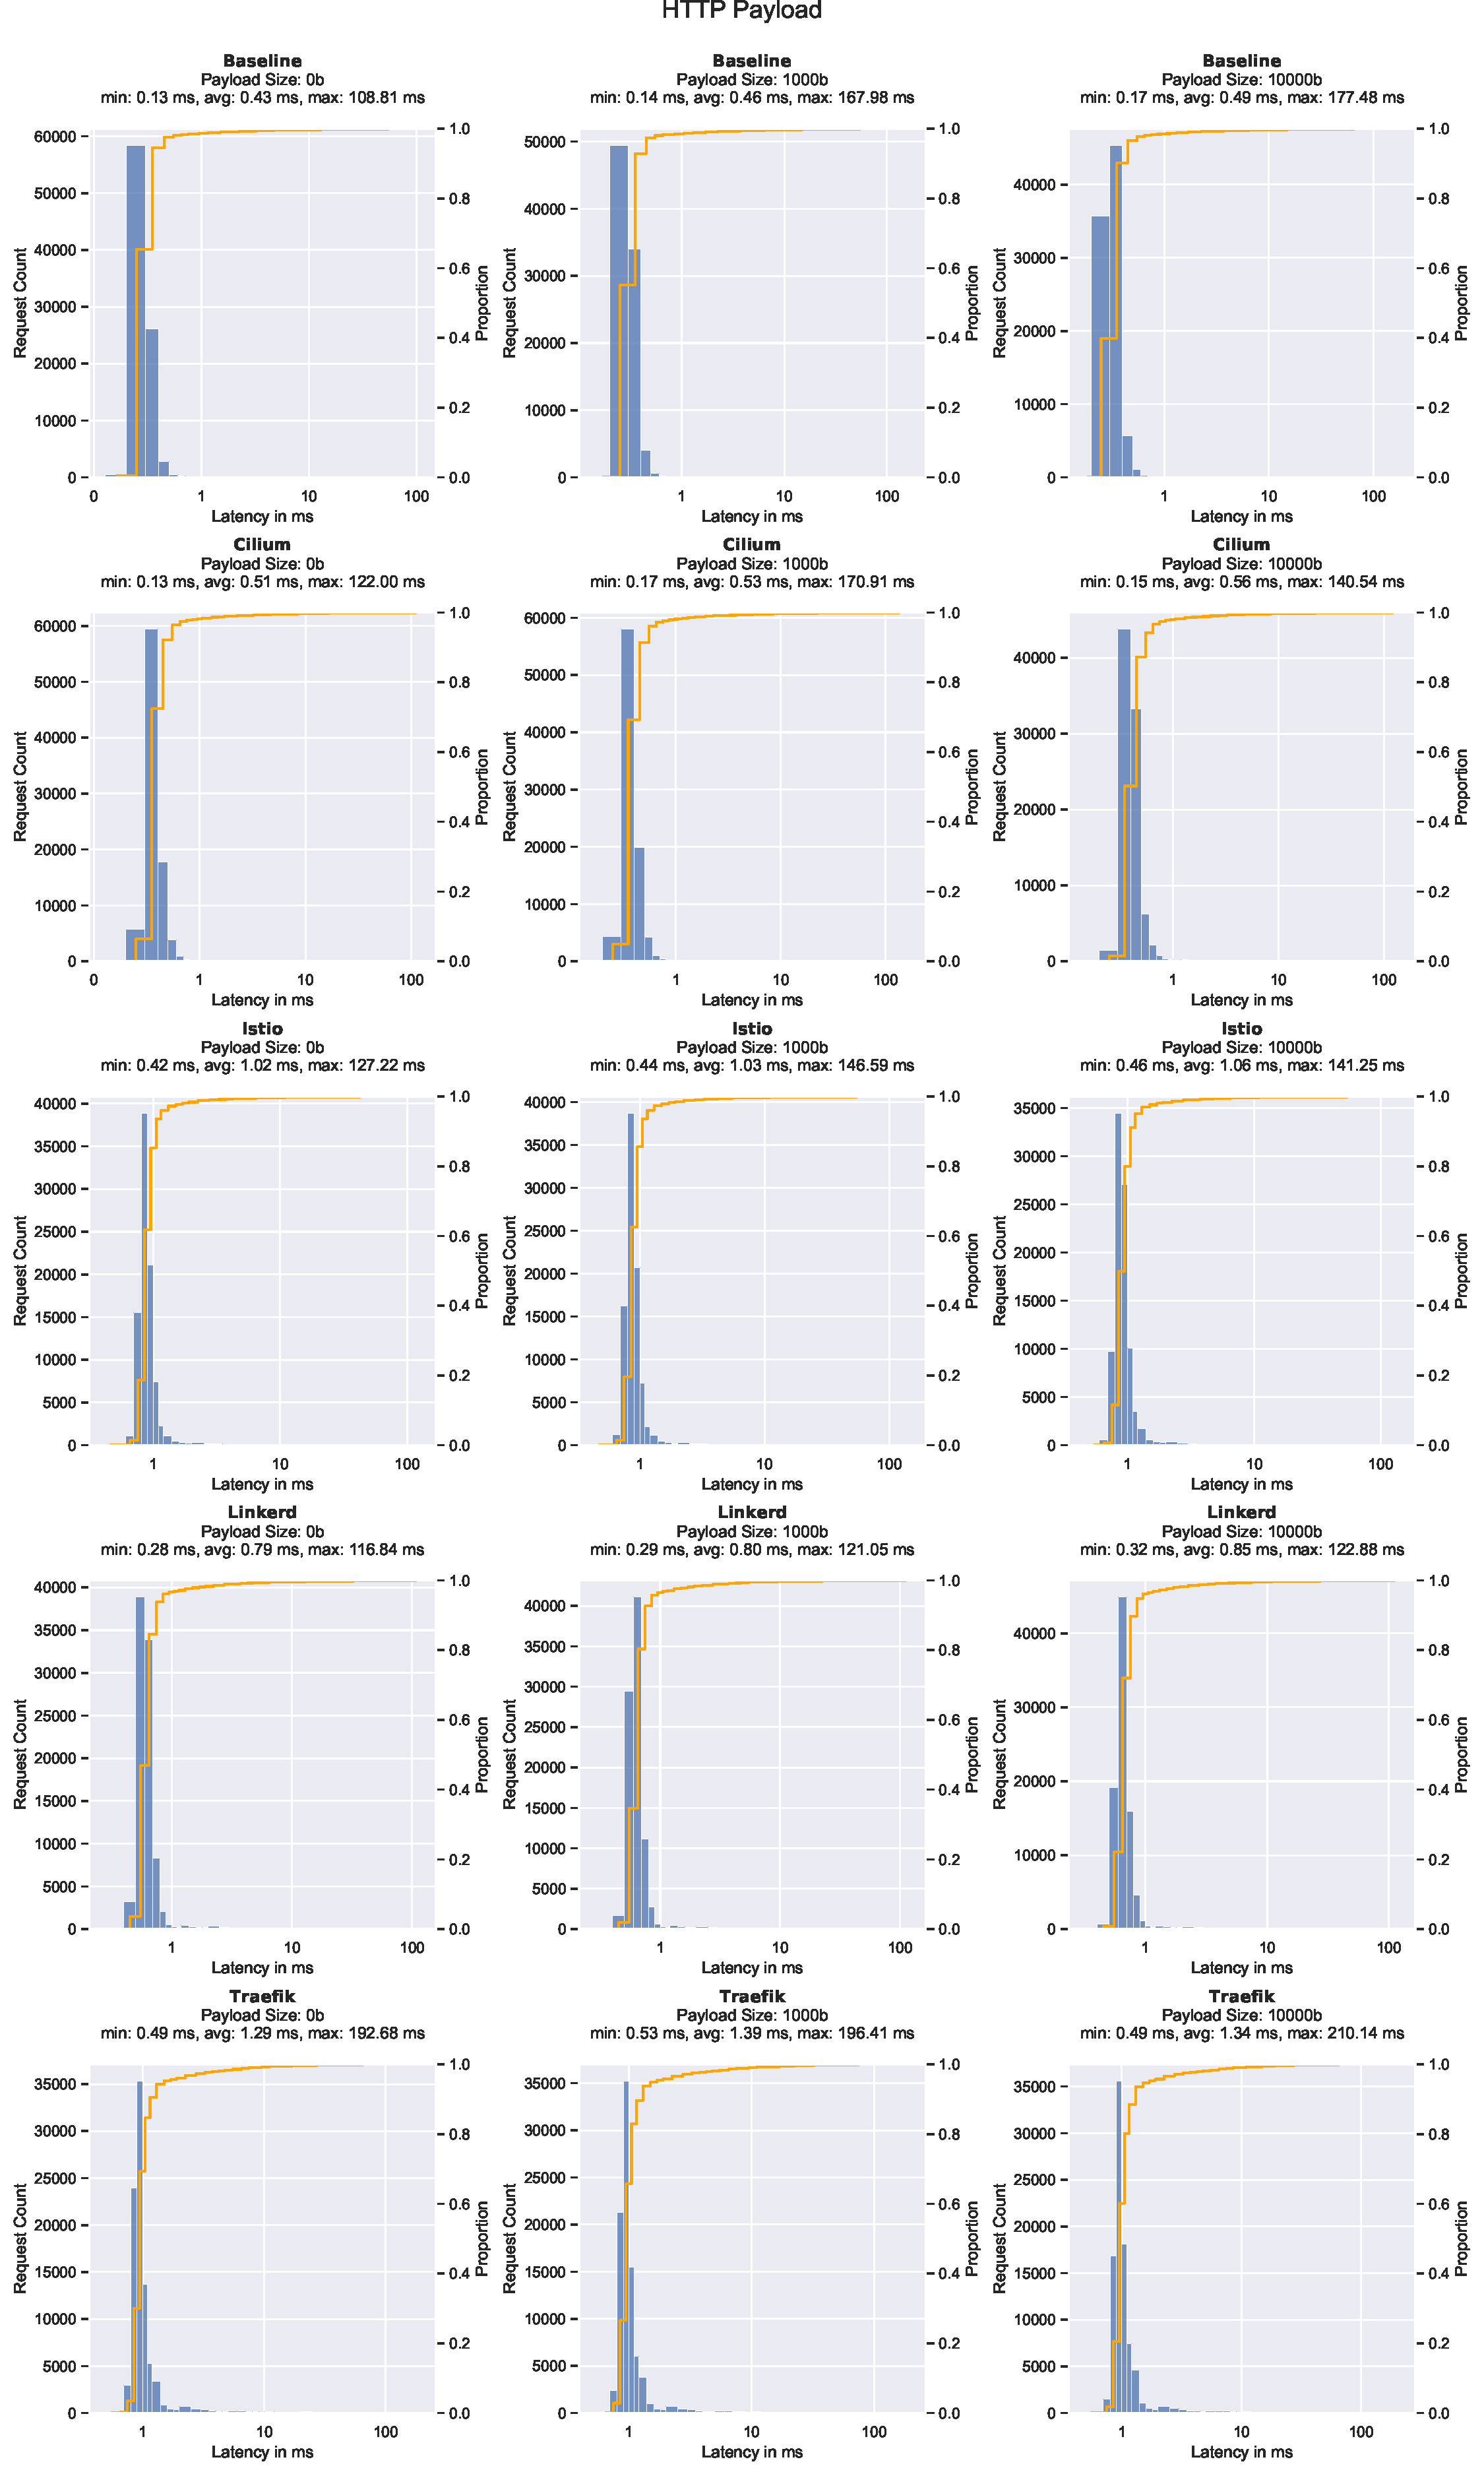
\includegraphics[width=\textwidth,height=\textheight]{5_experimental_evaluation/figures/exp_03-latency-results.pdf}

    \caption{\ref{exp:design:3} - Latency Results}
    
    \label{fig:exp:result:03:latency}
\end{figure}


% Results
% -maximum values higher
% p99.9 p99 similar
From the results of the histograms as depicted in \cref{fig:exp:result:03:latency} we can observe that the distributions remain similar for all the observed payload sizes. In fact, when inspecting the data in finer detail we observe that the tail end is nearly identical and that there is no significant difference in the tail latencies of the 99th and 99.9th percentile. 


\subsubsection{\ref{exp:design:4} - gRPC Maximum Throughput}
\label{sec:experiments:results:per-experiment:04}
% Goal: To evaluate how meshed configurations behave with alternative communication protocols.

The final experiment uses a different type of workload. In this experiment, we aim to evaluate the performance of \gls{sm} systems under alternative application level protocols. The results of this experiment can be seen in \cref{fig:exp:result:04:latency}


\begin{figure}[h]
    \centering
    
    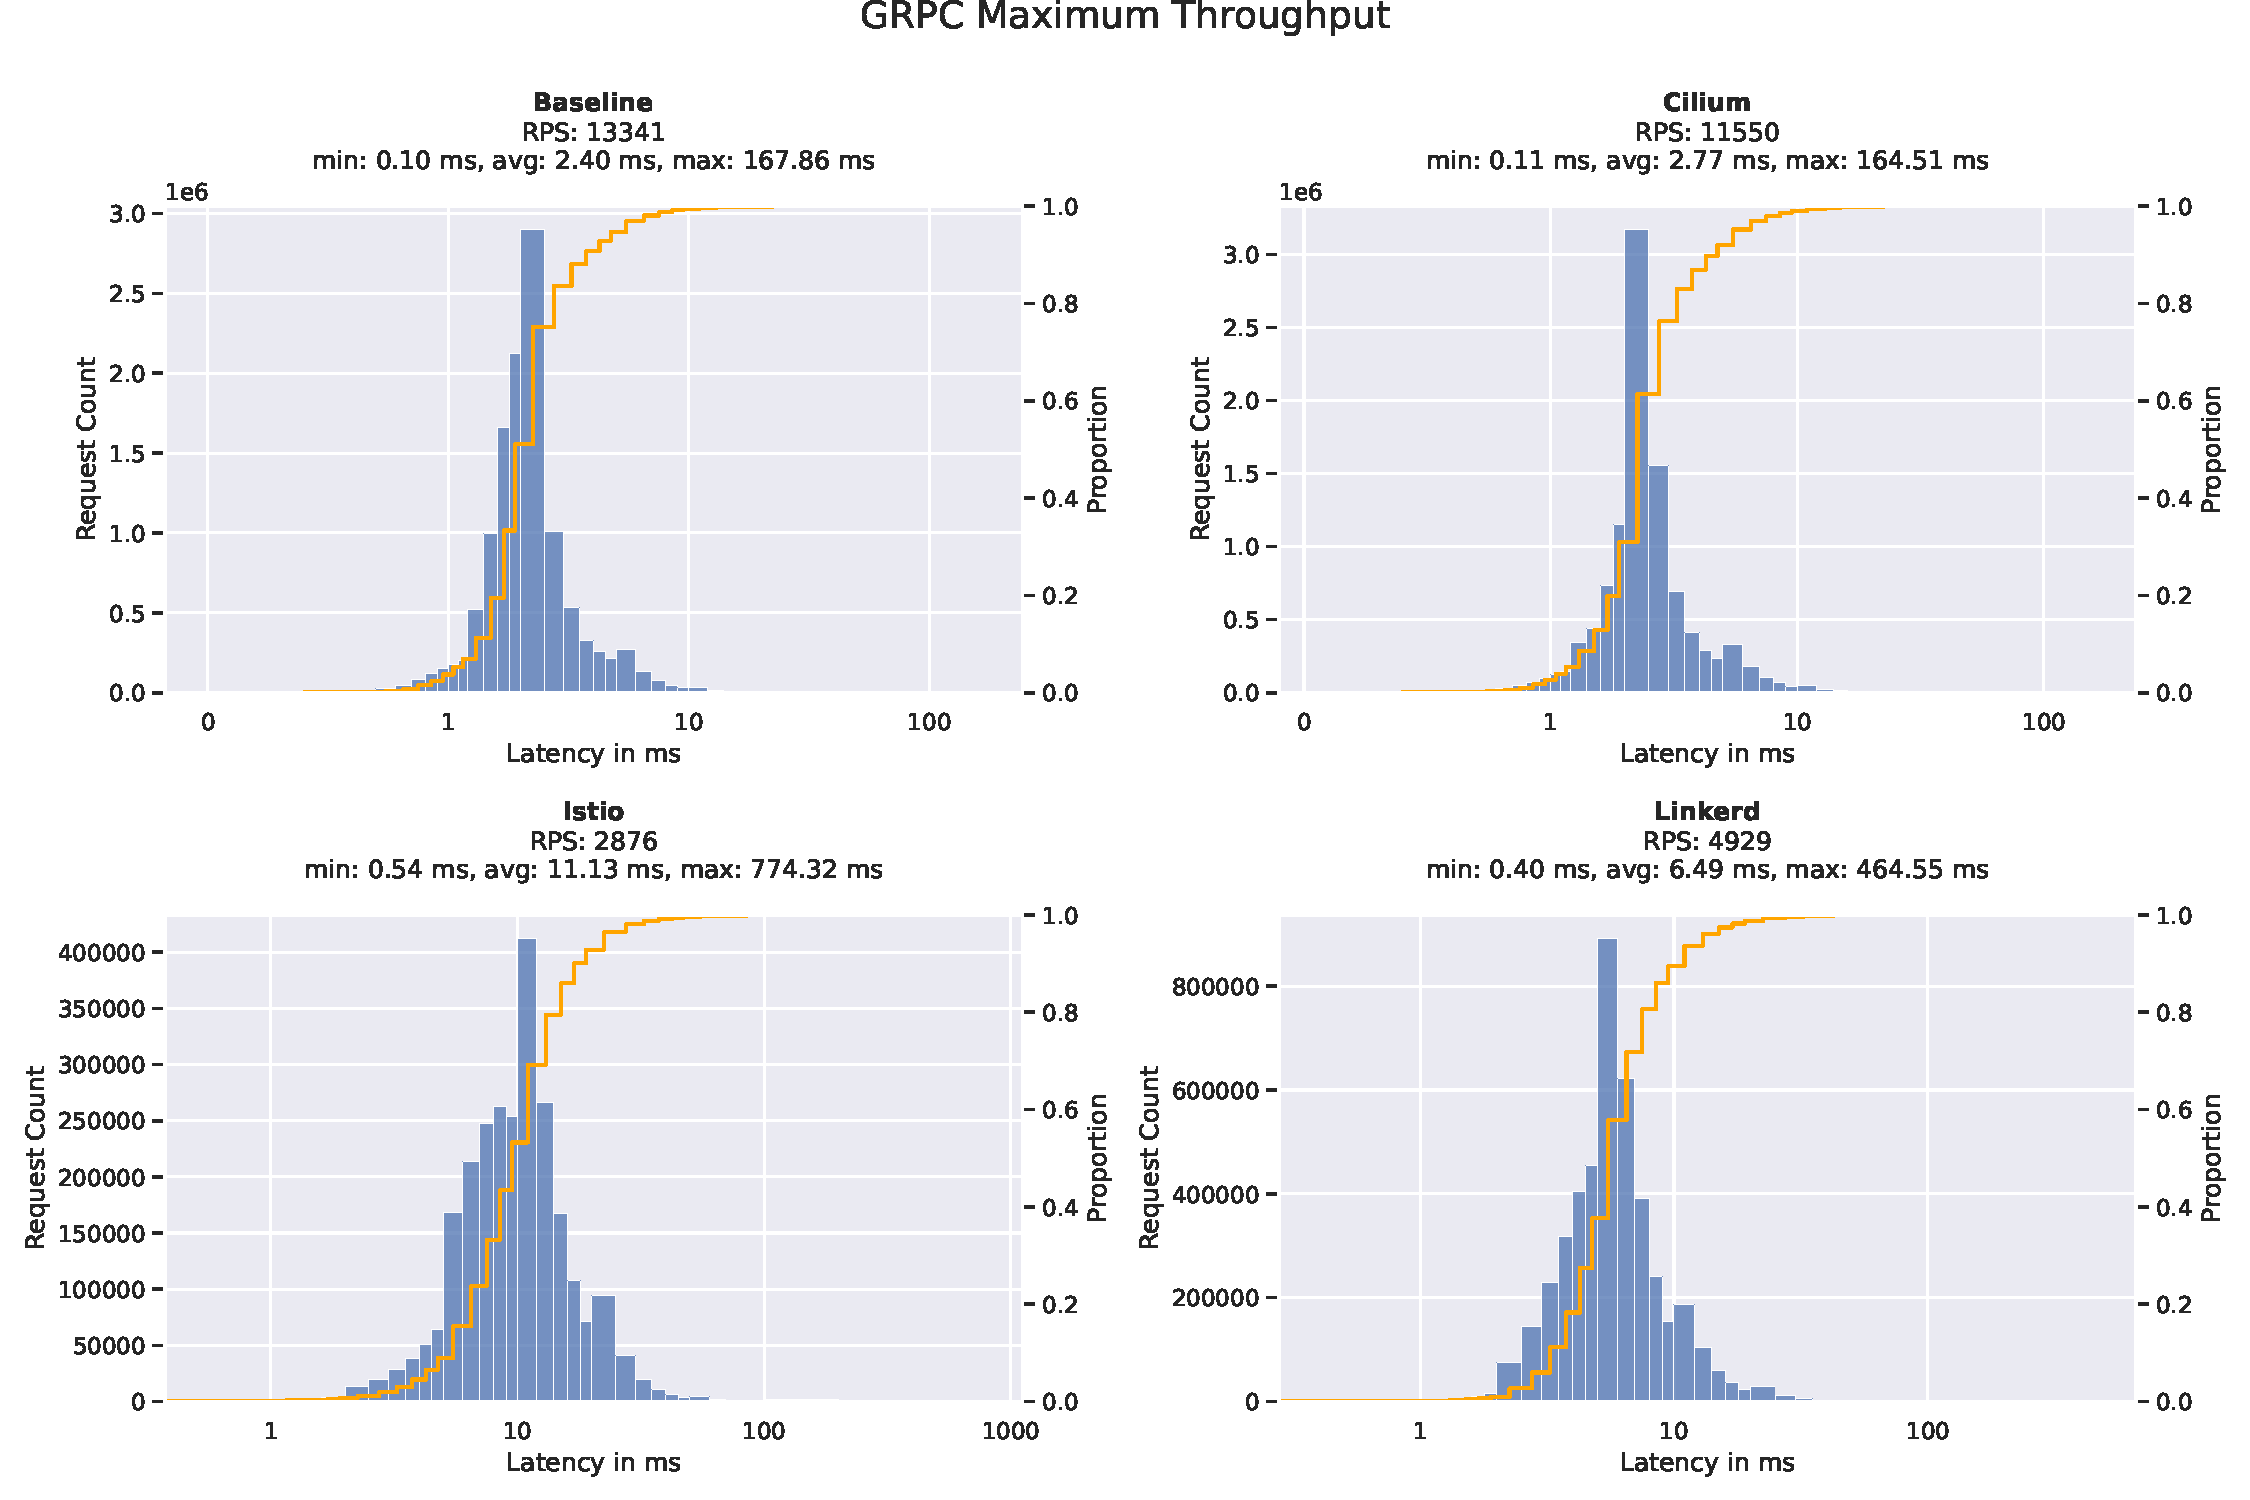
\includegraphics[width=\linewidth]{5_experimental_evaluation/figures/exp_04-latency-results.pdf}

    \caption{\ref{exp:design:4} - latency results.}
    
    \label{fig:exp:result:04:latency}
\end{figure}

% Describe plots
The histograms in \cref{fig:exp:result:04:latency} show the distribution of request latencies of the gRPC workloads for each of the mesh configurations. The y-axis on the left represents the number of requests related to the bars. The y-axis on the right indicates the proportion which is tied to the cumulative distribution function line on top of the histogram. The x-axis is once again a logarithmic axis representing the latency expressed in milliseconds. Additional descriptive metrics are presented above each plot and the actual amount of throughput reached is included as well expressed in requests per second (RPS).

% Results
% - No Traefik -> No support
% - High tail end latencies
% - Drops:
% cilium -13.424%
% istio: -78.442%
% linkerd: -63.053%

% Htpt diff
% % cilium QPS diff: -16.827679769486704%
% istio QPS diff: -80.0264142981776%
% linkerd QPS diff: -54.940993873502805%
% traefik QPS diff: -97.38692130213765%
The first observation from this experiment was that the \textit{Traefik} proxy was unable to support and therefore process the gRPC requests, leading to its absence in the depicted results. Furthermore, we can see that for the meshed configurations we again see a decrease in maximum throughput achieved compared to the baseline configuration for all the meshed configurations. Similar to the HTTP experiment as discussed in \cref{sec:experiments:results:per-experiment:01}, we observe that \textit{Cilium} is performing the best out of all meshed configurations regarding its maximum throughput, losing out on $-13.42\%$ compared to the baseline. \textit{Linkerd} and \textit{Istio} have a significant drop compared to the baseline configuration, losing $-54.94\%$ and $-97.39\%$ of the maximum throughput compared to the baseline respectively. An interesting observation can be made is regarding the distributions and tail end latencies of the requests for \textit{Linkerd} and \textit{Istio}. The average requests latencies see a significant increase, with $+170.42\%$ and $+363.75\%$ compared to the baseline average respectively. This trend continues for the tail end latencies and maximum values observed as well indicating that the proxies introduce a notable performance overhead.

% istio ~38 p99
% linkerd ~22 p99
\section{Discussion}
\label{sec:experiments:discussion}
	

% Setup
\graphicspath{./figures}

\chapter{Conclusion and Future Work}
\label{chap:conclusion}

\section{Conclusion}
\label{sec:conclusion:conclusion}

\cite{test-online}
\cite{test-software}



\section{Future Work}
\label{sec:conclusion:future-work}
          
\chapter*{Appendix}
\todo{Print glossary entries when finalizing document.}
% Uncomment for sorted glossary definitions
% \printglossaries


\includepdf[landscape, pagecommand={}\label{appendix:cncf-landscape}]{9_appendix/figures/cncf-landscape.pdf}


\section{Experiment Overview}
\begin{table}[!t]
    \centering

    \begin{tabularx}{\textwidth}{l X}
    
        \toprule
        \multicolumn{2}{c}{\textbf{EXP 1 - HTTP Maximum Throughput}}  \\
        \toprule
        
        \textbf{Goal}
        & To find the maximum throughput each of the meshed configurations can achieve. \\
        \midrule
        
        \textbf{Methodology}
        & The load generator will run in an unrestricted mode and generate as much load as possible without holding back and without any request timeouts. The maximum throughput is determined by looking at the actual number of requests per second in the configuration was able to achieve. \\
        \midrule
        
        \textbf{Workload} 
        & HTTP (\cref{sec:experiments:design:workloads:http}) \\
        \midrule

        \multirow{1}{*}{\textbf{Factors}} 
        & \Gls{sm} configuration (\cref{sec:experiments:design:meshes}) \\
        \midrule
        
        \textbf{Reasoning}
        & This experiment will serve as a baseline to determine the maximum throughput of all meshed configurations. The results will be used to determine sensible defaults for the experiments with a pre-defined constant throughput. \\

        \bottomrule

    \end{tabularx}
    \caption[Experiment Design: Experiment 1.]{Experiment Design: Experiment 1.}
    \label{tab:experiment:design:01}
\end{table}
\begin{table}[!t]
    \centering

    \begin{tabularx}{\textwidth}{l X}
    
        \toprule
        \multicolumn{2}{c}{\textbf{EXP 2 - HTTP Constant Throughput}}  \\
        \toprule
        
        \textbf{Goal}
        & To evaluate how \gls{sm} configurations behave under varying levels of load. \\
        \midrule
        
        \textbf{Methodology}
        & The load generator will generate load in a constant and uniform throughput setting. This means that the load generator will produce a set number of requests per second and will not deviate or try to catch up when requests are not processed in time.  \\
        \midrule
        
        \textbf{Workload} 
        & HTTP (\cref{sec:experiments:design:workloads:http}) \\
        \midrule

        \multirow{2}{*}{\textbf{Factors}} 
        & \Gls{sm} configuration (\cref{sec:experiments:design:meshes}) \\
        & Requests per second \\
        \midrule
        
        \textbf{Reasoning}
        & This experiment evaluates the \gls{sm} configurations under similar levels of load. This allows us to compare these configurations to one another when they undergo the same workloads.  \\

        \bottomrule

    \end{tabularx}
    \caption[Experiment Design: Experiment 2.]{Experiment Design: Experiment 2.}
    \label{tab:experiment:design:02}
\end{table}
\begin{table}[!t]
    \centering

    \begin{tabularx}{\textwidth}{l X}
    
        \toprule
        \multicolumn{2}{c}{\textbf{EXP 3 - HTTP Payload Response}}  \\
        \toprule
        
        \textbf{Goal}
        & To evaluate how \gls{sm} configurations behave with varying payload sizes. \\
        \midrule
        
        \textbf{Methodology}
        & The load generator will produce HTTP requests to the target service, which in turn will respond with pre-determined payload sizes.  \\
        \midrule
        
        \textbf{Workload} 
        & HTTP (\cref{sec:experiments:design:workloads:http}) \\
        \midrule

        \multirow{2}{*}{\textbf{Factors}} 
        & \Gls{sm} configuration (\cref{sec:experiments:design:meshes}) \\
        & Payload size \\
        \midrule
        
        \textbf{Reasoning}
        & This experiment introduces several pre-determined payload sizes to evaluate the effects of additional application data being transferred in meshed environments. This allows us to study the effects and potential additional overheads extra data transferes may cause. \\

        \bottomrule

    \end{tabularx}
    \caption[Experiment Design: Experiment 3.]{Experiment Design: Experiment 3.}
    \label{tab:experiment:design:03}
\end{table}
\begin{table}[!t]
    \centering

    \begin{tabularx}{\textwidth}{l X}
    
        \toprule
        \multicolumn{2}{c}{\textbf{EXP 4 - gRPC Maximum Throughput}}  \\
        \toprule
        
        \textbf{Goal}
        & To evaluate how meshed configurations behave with alternative communication protocols. \\
        \midrule
        
        \textbf{Methodology}
        & The load generator will generate gRPC traffic towards the gRPC service and do so in an unrestricted manner, meaning it will try to generate as much load as possible without holding back and without enforcing any timeouts. The maximum throughput is determined by looking at the actual number of requests per second in the configuration was able to achieve. \\
        \midrule
        
        \textbf{Workload} 
        & gRPC (\cref{sec:experiments:design:workloads:grpc}) \\
        \midrule

        \multirow{1}{*}{\textbf{Factors}} 
        & \Gls{sm} configuration (\cref{sec:experiments:design:meshes}) \\
        \midrule
        
        \textbf{Reasoning}
        & This experiment allows us to evaluate the effects of alternative application level protocols. During the system survey we uncovered that \gls{sm} systems inspect and use this data to for both observability and routing functionalities. This experiment allows us to uncover the effects of alternative, but common, application level protocols widely used within the industry. \\

        \bottomrule

    \end{tabularx}
    \caption[Experiment Design: Experiment 4.]{Experiment Design: Experiment 4.}
    \label{tab:experiment:design:04}
\end{table}

\section{Experiment 1 Results}

\begin{figure}[h]
    \centering
    
    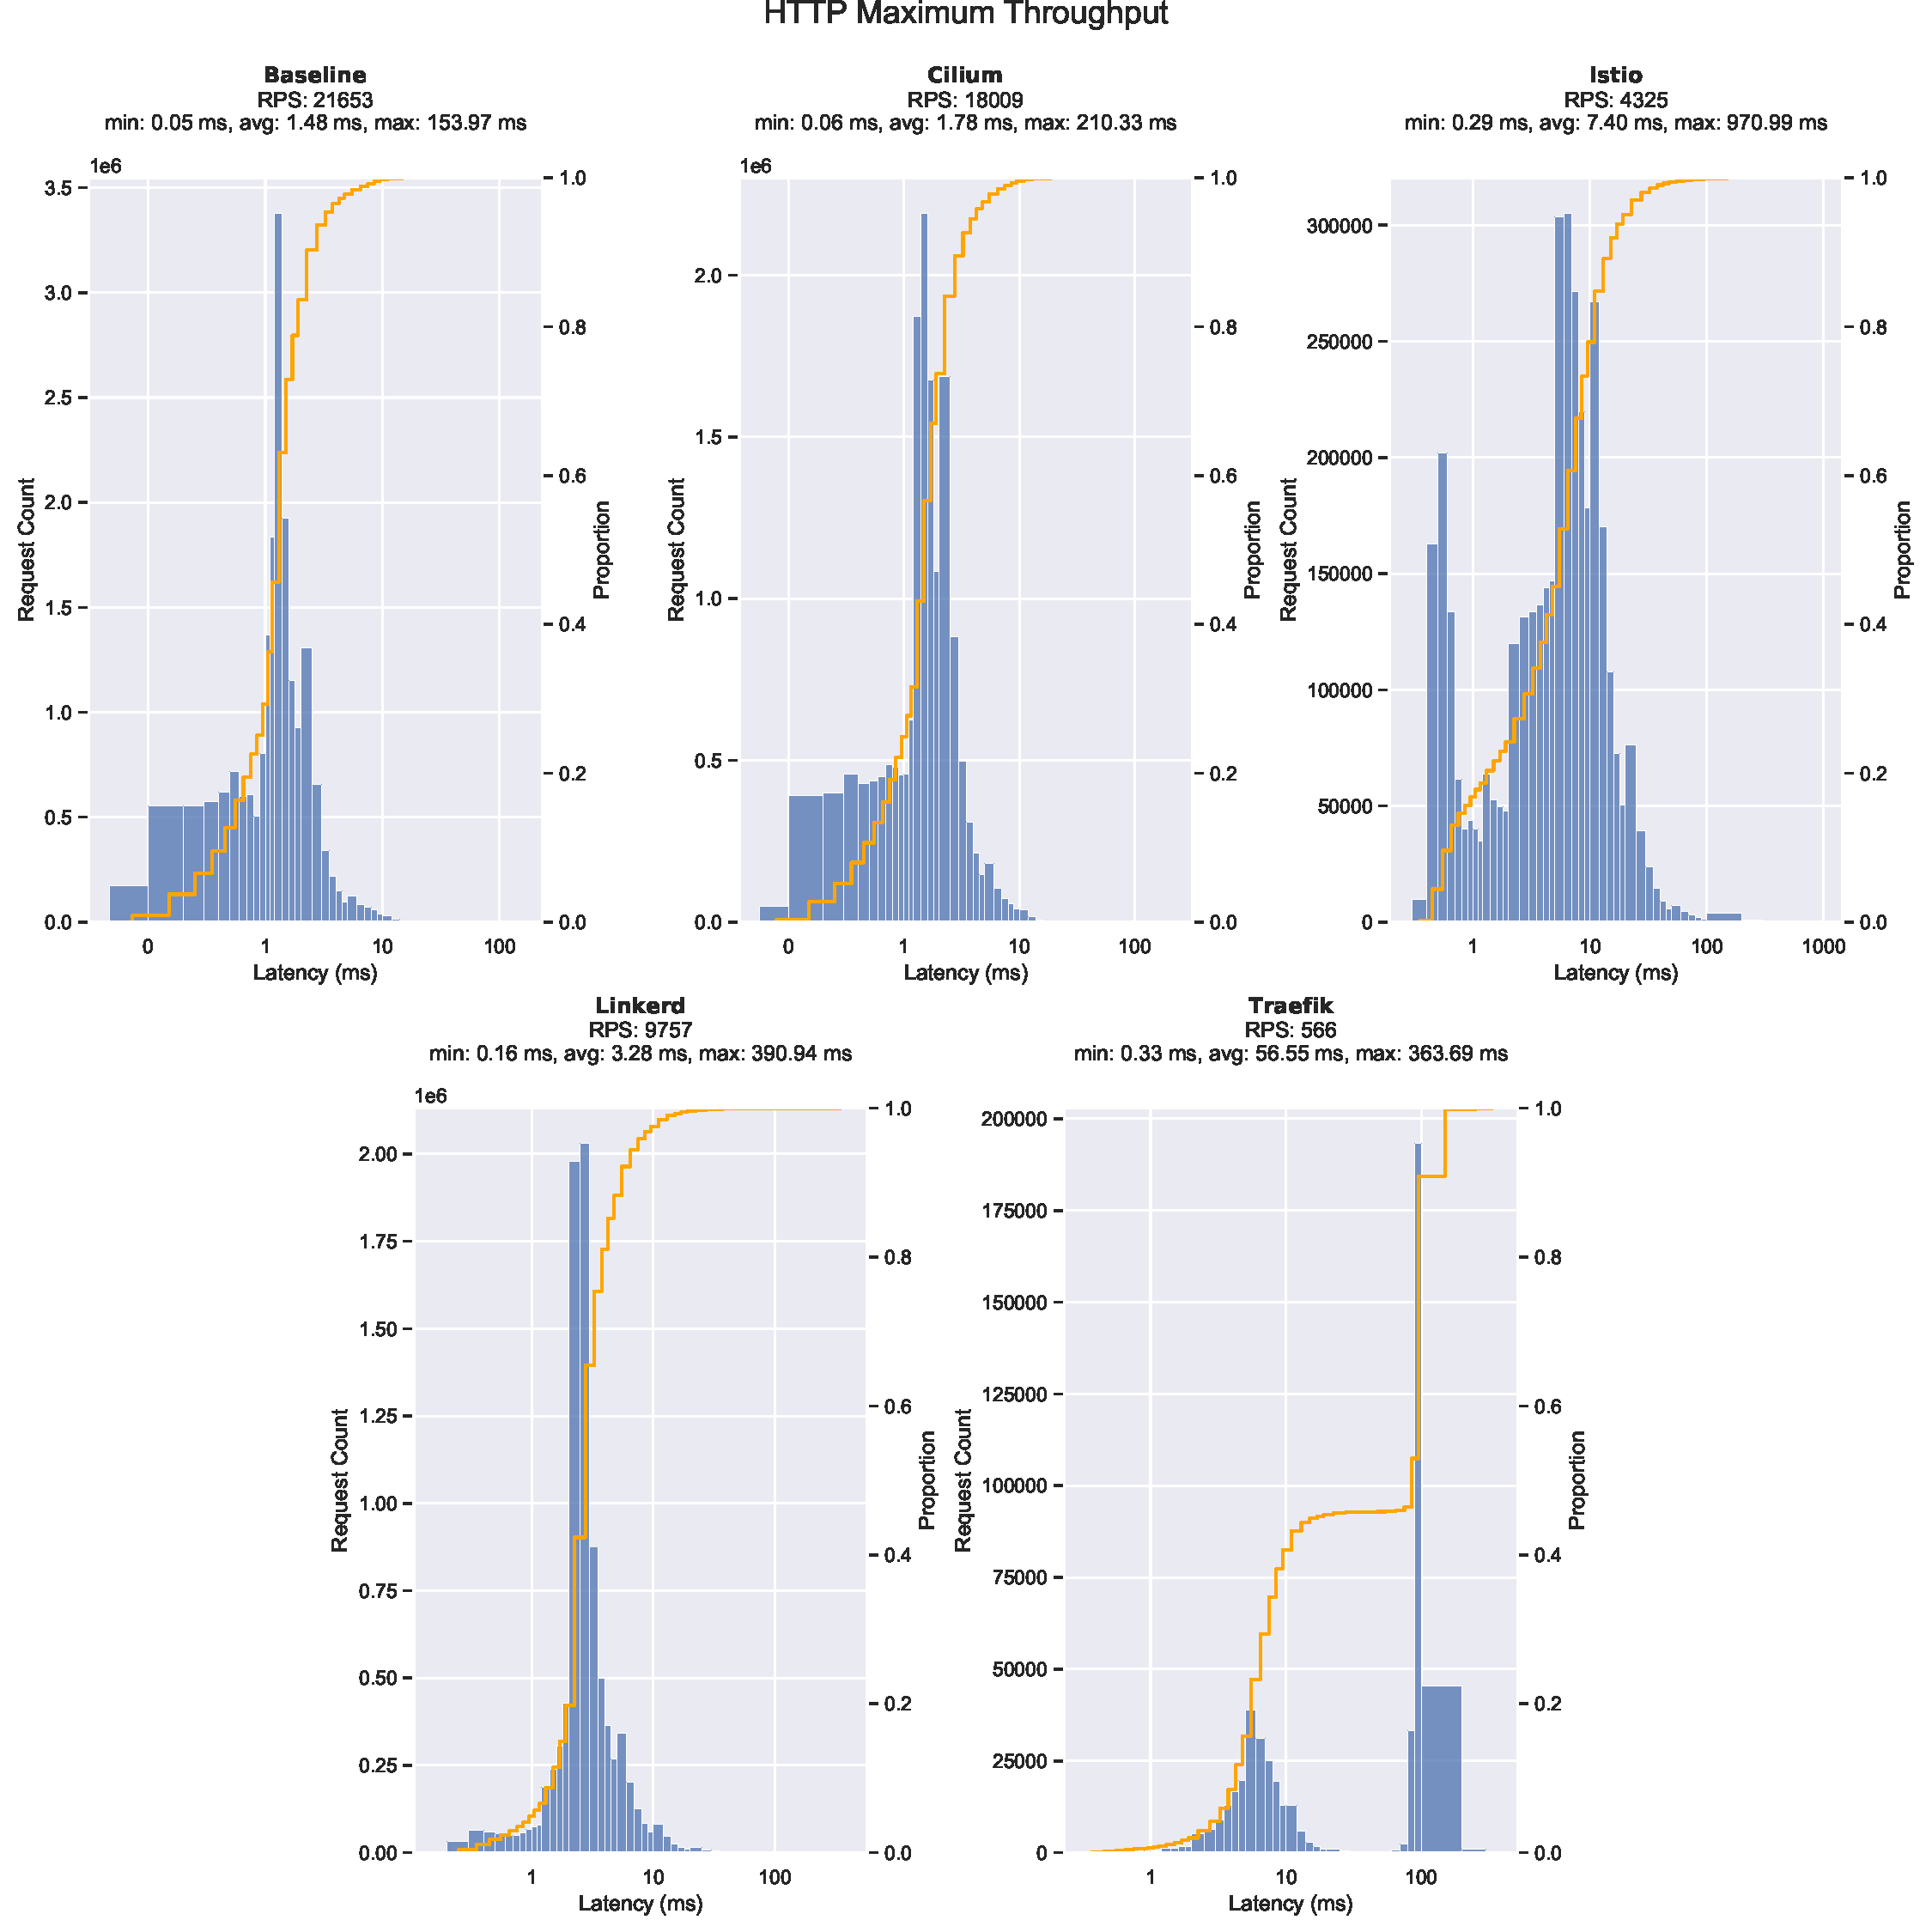
\includegraphics[width=\linewidth]{5_experimental_evaluation/figures/exp_01-latency-results.pdf}

    \caption{\ref{exp:design:1} - Histogram - Latency per Service Mesh.}
    
    \label{fig:appendix:exp:result:01:latency:histogram}
\end{figure}

\begin{figure}[h]
    \centering
    
    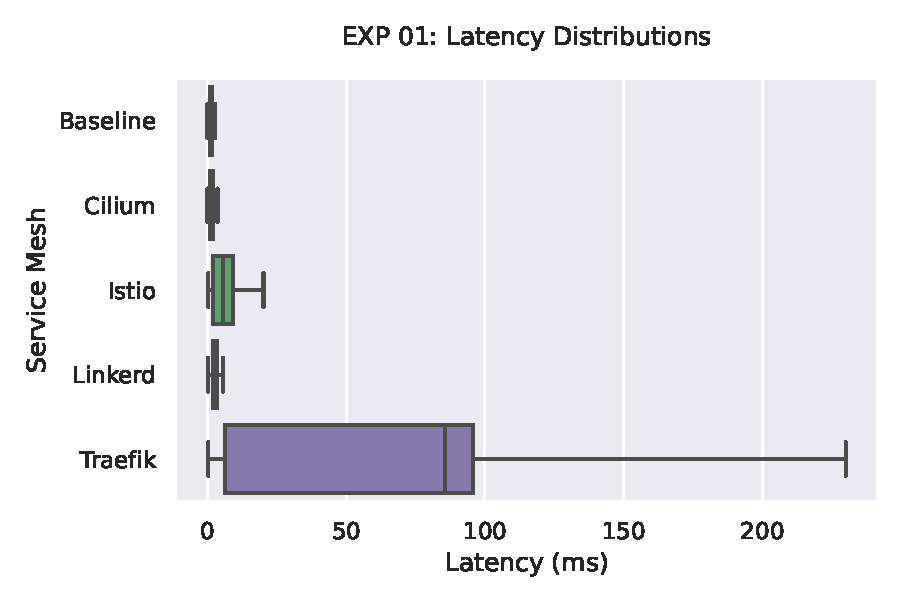
\includegraphics[width=\linewidth]{5_experimental_evaluation/figures/exp_01-latency-boxplot.pdf}

    \caption{\ref{exp:design:1} - Box plot - Latency per Service Mesh.}
    
    \label{fig:appendix:exp:result:01:latency:boxplot}
\end{figure}


\begin{figure}[h]
    \centering
    
    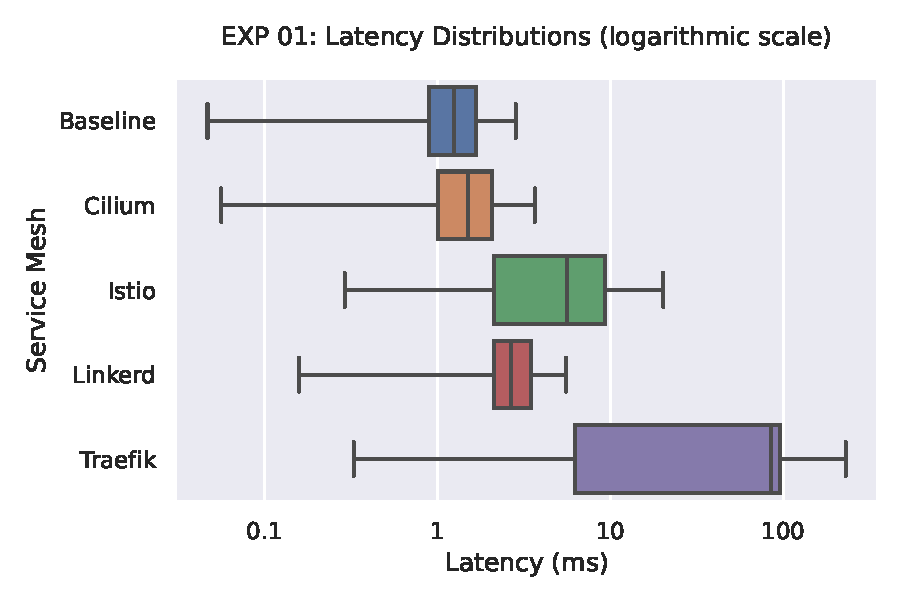
\includegraphics[width=\linewidth]{5_experimental_evaluation/figures/exp_01-latency-boxplot-log.pdf}

    \caption{\ref{exp:design:1} - Box plot - Latency per Service Mesh (logarithmic scale).}
    
    \label{fig:appendix:exp:result:01:latency:boxplot-log}
\end{figure}

\begin{figure}[h]
    \centering
    
    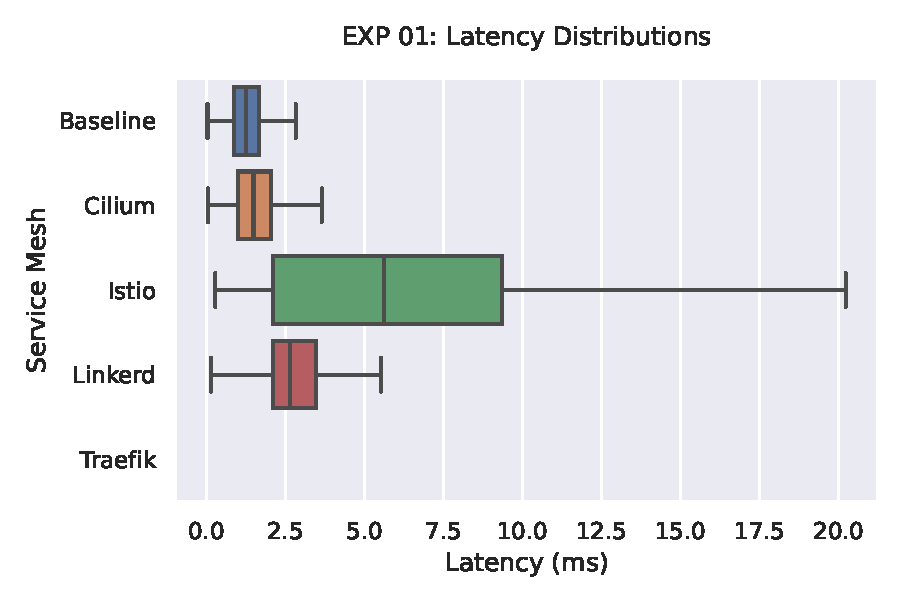
\includegraphics[width=\linewidth]{5_experimental_evaluation/figures/exp_01-latency-boxplot-no-traefik.pdf}

    \caption{\ref{exp:design:1} - Box plot - Without Traefik.}
    
    \label{fig:appendix:exp:result:01:latency:boxplot-no-traefik}
\end{figure}


\begin{figure}[h]
    \centering
    
    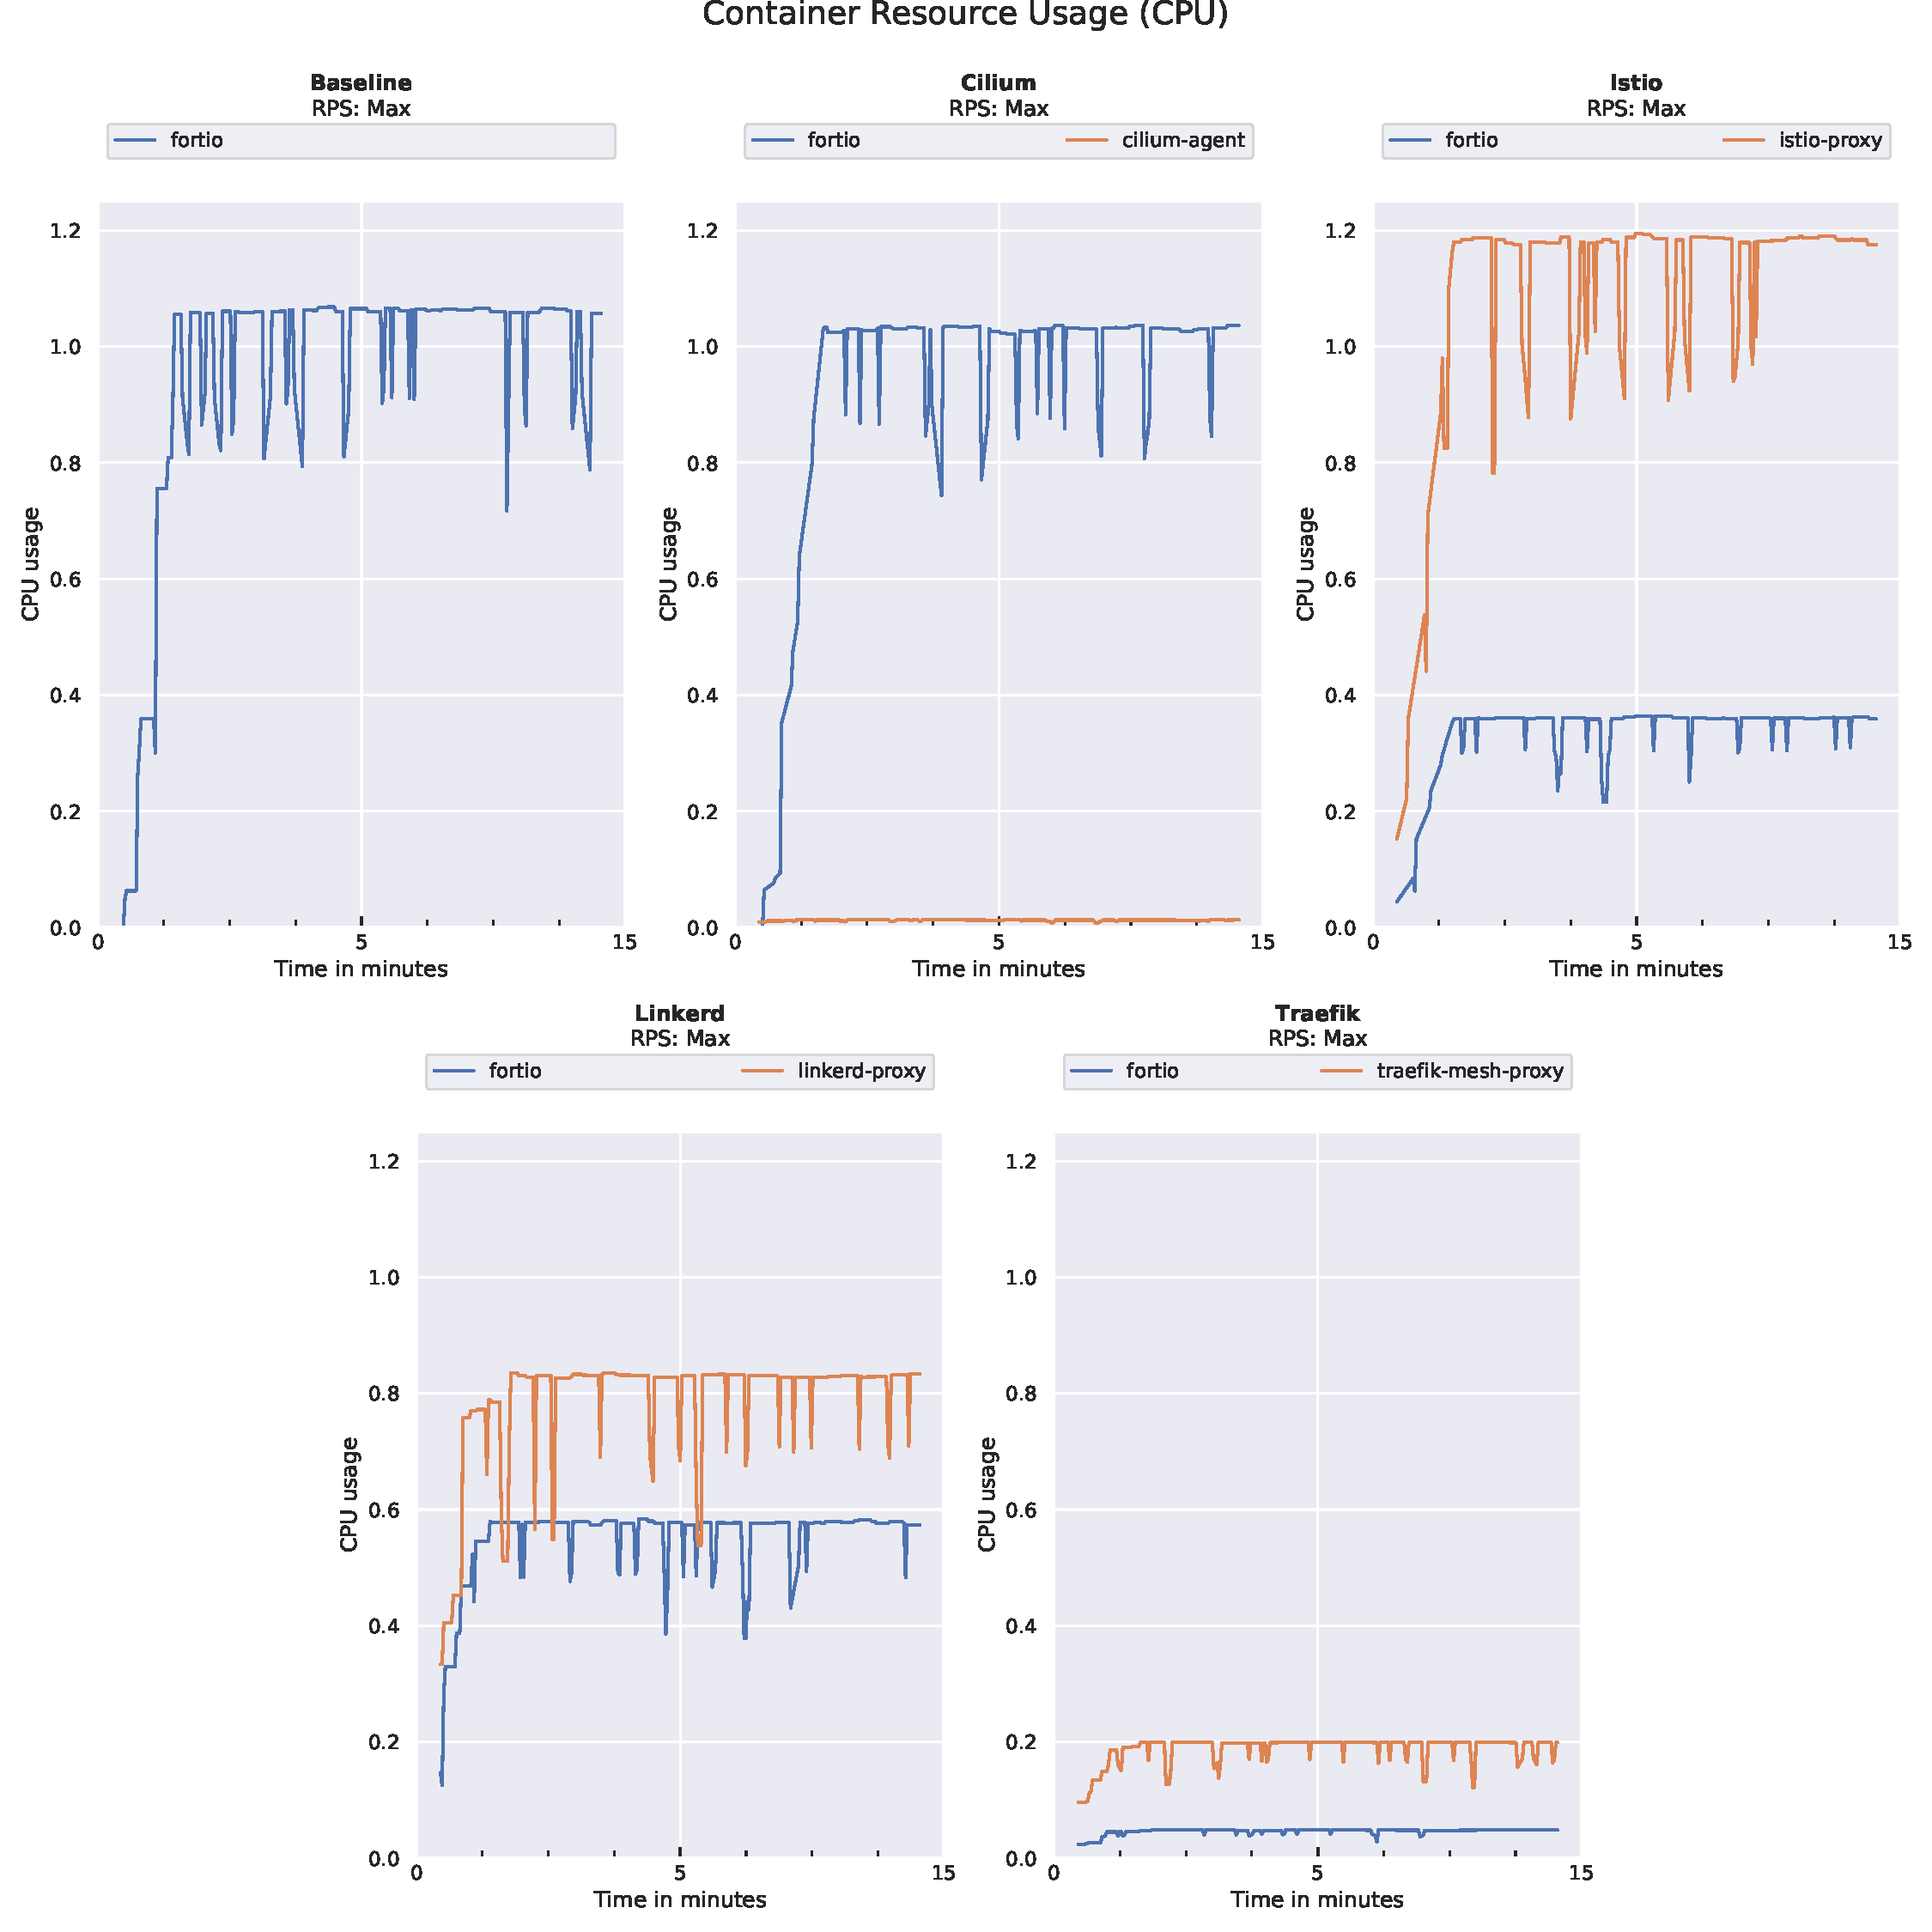
\includegraphics[width=\linewidth]{5_experimental_evaluation/figures/exp_01-cpu-results.pdf}

    \caption{\ref{exp:design:1} - CPU utilization over time.}
    
    \label{fig:appendix:exp:result:01:cpu:timeline}
\end{figure}


\begin{figure}[h]
    \centering
    
    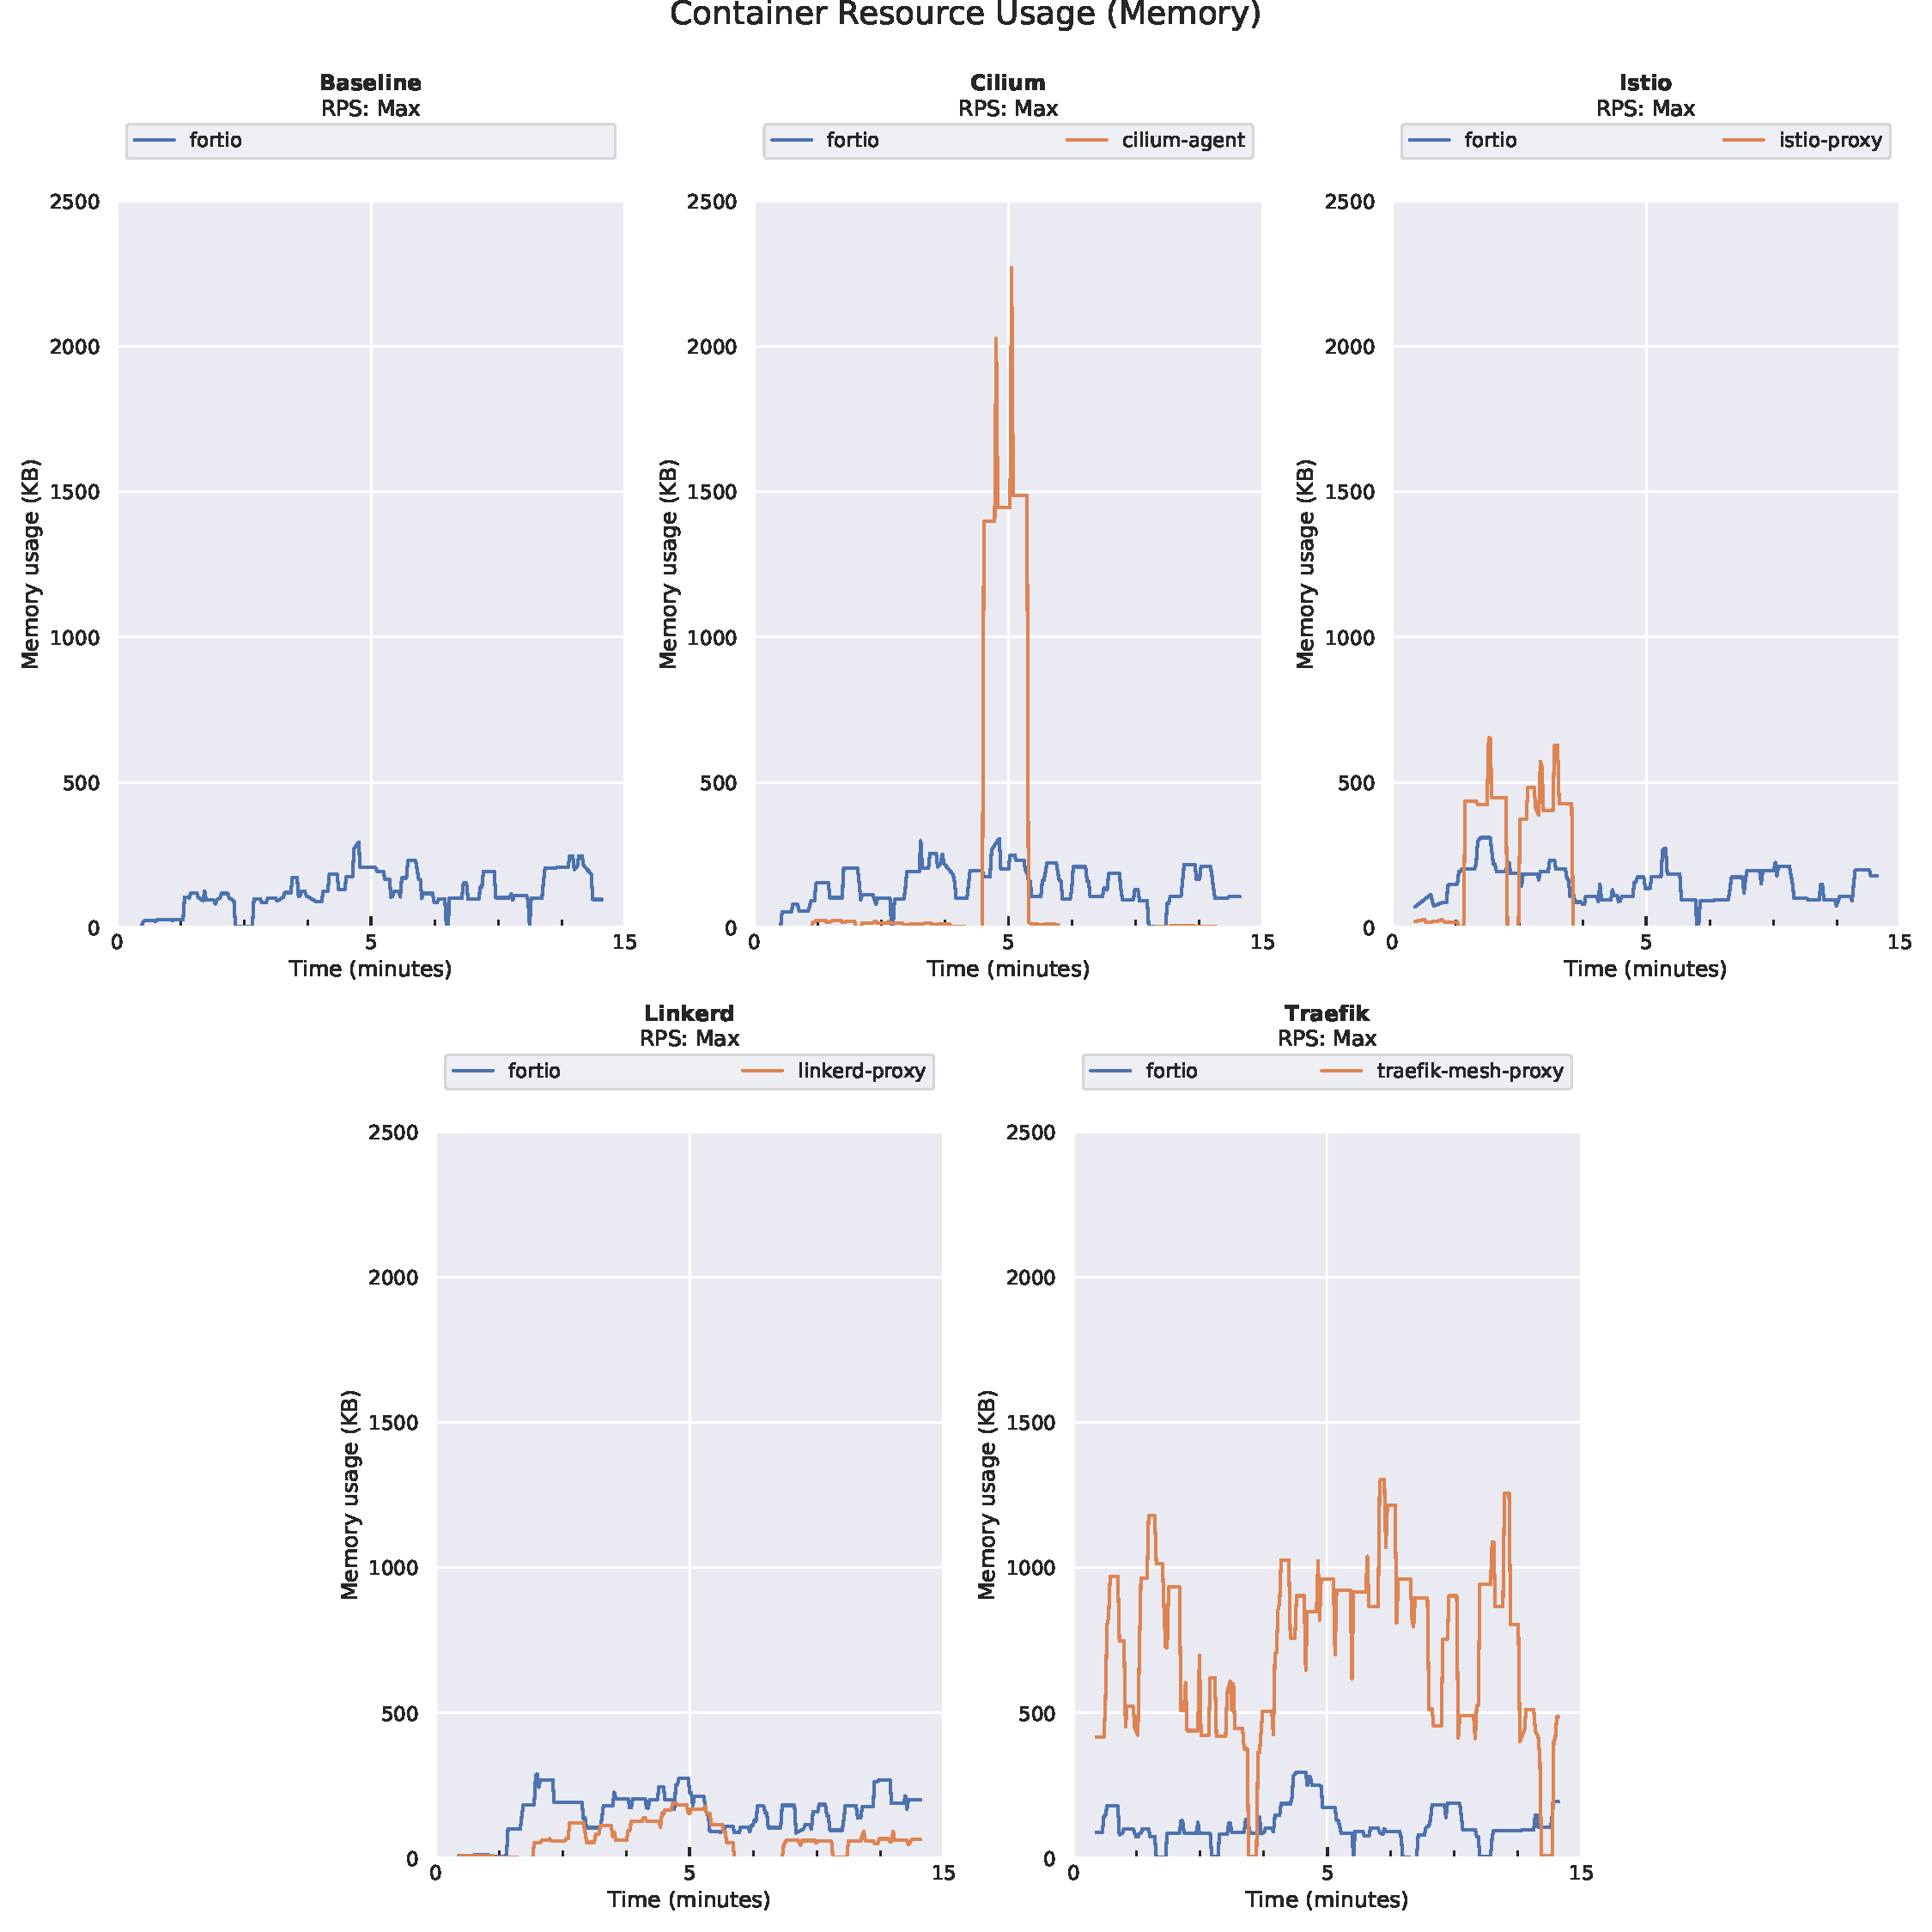
\includegraphics[width=\linewidth]{5_experimental_evaluation/figures/exp_01-memory-results.pdf}

    \caption{\ref{exp:design:1} - Memory consumption over time.}
    
    \label{fig:appendix:exp:result:01:memory:timeline}
\end{figure}


\begin{figure}[h]
    \centering
    
    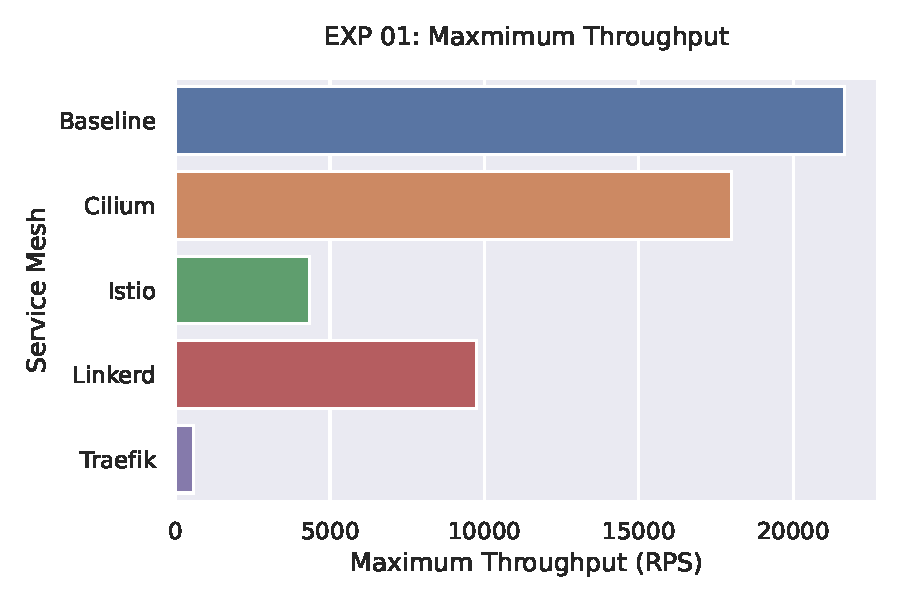
\includegraphics[width=\linewidth]{5_experimental_evaluation/figures/exp_01-throughput-barchart.pdf}

    \caption{\ref{exp:design:1} - Bar Chart - Maximum Throughput per mesh.}
    
    \label{fig:appendix:exp:result:01:throughput:barchart}
\end{figure}


\section{Experiment 2 Results}

\begin{figure}[h]
    \centering
    
    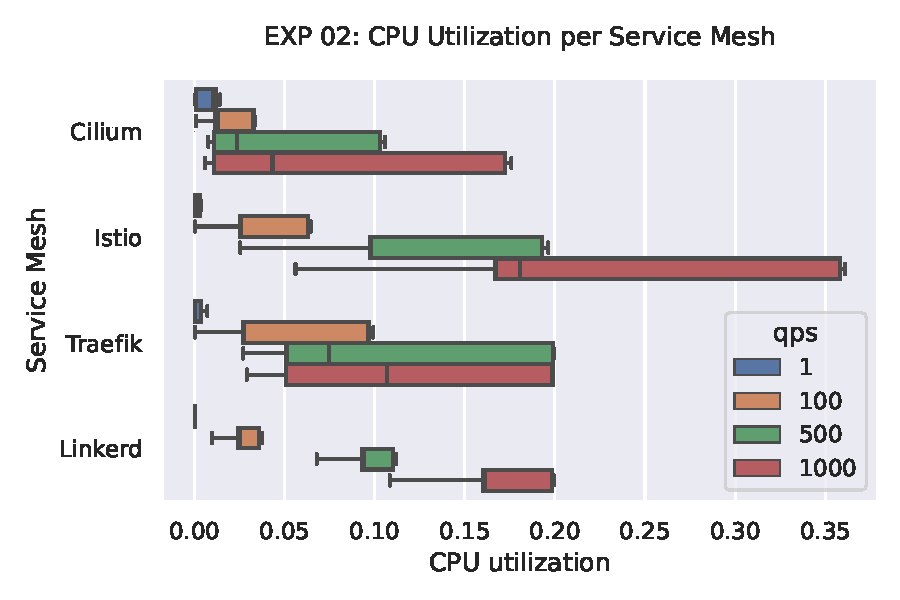
\includegraphics[width=\linewidth]{5_experimental_evaluation/figures/exp_02-cpu-boxplot.pdf}

    \caption{\ref{exp:design:2} - Box Plot - CPU utilization.}
    
    \label{fig:appendix:exp:result:02:cpu-boxplot}
\end{figure}


\section{Experiment 3 Results}

\section{Experiment 4 Results}

      
            
% --------------------------------------------------------------
%:                  BACK MATTER: appendices, refs,..
% --------------------------------------------------------------

% the back matter: appendix and references close the thesis


%: ----------------------- bibliography ------------------------

% The section below defines how references are listed and formatted
% The default below is 2 columns, small font, complete author names.
% Entries are also linked back to the page number in the text and to external URL if provided in the BibTex file.

% PhDbiblio-url2 = names small caps, title bold & hyperlinked, link to page 
%\begin{multicols}{2} % \begin{multicols}{ # columns}[ header text][ space]
%\begin{tiny} % tiny(5) < scriptsize(7) < footnotesize(8) < small (9)

\bibliographystyle{Latex/Classes/PhDbiblio-url2} % Title is link if provided
\renewcommand{\bibname}{References} % changes the header; default: Bibliography

\bibliography{7_references/references} % adjust this to fit your BibTex file

%\end{tiny}
%\end{multicols}



% --------------------------------------------------------------
% Various bibliography styles exit. Replace above style as desired.

% in-text refs: (1) (1; 2)
% ref list: alphabetical; author(s) in small caps; initials last name; page(s)
%\bibliographystyle{Latex/Classes/PhDbiblio-case} % title forced lower case
%\bibliographystyle{Latex/Classes/PhDbiblio-bold} % title as in bibtex but bold
%\bibliographystyle{Latex/Classes/PhDbiblio-url} % bold + www link if provided

%\bibliographystyle{Latex/Classes/jmb} % calls style file jmb.bst
% in-text refs: author (year) without brackets
% ref list: alphabetical; author(s) in normal font; last name, initials; page(s)

%\bibliographystyle{plainnat} % calls style file plainnat.bst
% in-text refs: author (year) without brackets
% (this works with package natbib)


% --------------------------------------------------------------

% according to Dresden med fac summary has to be at the end
%
% Thesis Abstract -----------------------------------------------------


%\begin{abstractslong}    %uncommenting this line, gives a different abstract heading
\begin{abstracts}        %this creates the heading for the abstract page
Service-oriented computing, an architectural approach of decomposing software into logical services, has seen an increase in popularity over the past decades. Later forms, such as the widely popular microservices-based architecture is an evolution of service-oriented computing made possible by the reductions in deployment costs and resource overhead. These architectures offer advantageous characteristics, such as an increase in flexibility and scalability. However, due to its design, it also introduces an additional layer of complexity due to the overhead in communication and the inherent reliability issues from networks. The service mesh architecture tries aims to solve these issues whilst providing a uniform way of handling security, observability, and reliability concerns without modifying application code. In this thesis, we dissect the state-of-the service mesh systems and identify three different service mesh architectures. Furthermore, we design \textit{Mesh Bench} a benchmark used to evaluate the performance characteristics of service mesh systems. We implement a prototype of the benchmark and take an experimental approach to evaluating the most popular service mesh implementations in the form of \textit{Istio} and \textit{Linkerd}, and implementations using vastly different architectures in the form of \textit{Cilium} and \textit{Traefik mesh}. Based on the results of the performance experiments we uncover the performance overheads of service mesh systems and identify promising, future directions and evolutions of the techonology.

\end{abstracts}
%\end{abstractlongs}


% ---------------------------------------------------------------------- 


%: Declaration of originality
%\include{8_backmatter/declaration}

\end{document}
